\chapter[Namelist options]{\hyperref[chap:namelist_sections]{Namelist options}}
\label{chap:namelist_tables}
Embedded links point to more detailed namelist information in the appendix.
\section[run\_modes]{\hyperref[sec:nm_sec_run_modes]{run\_modes}}
\label{sec:nm_tab_run_modes}
MPAS-Ocean may be run in forward or analysis mode.  Forward mode is the default, and invokes the time stepping routine to run through the specified time duration.  Analysis mode simply reads in files upon initialization, runs all enabled analysis members, writes output, and shuts down.

\vspace{0.5in}
{\small
\begin{center}
\begin{longtable}{| p{2.0in} || p{4.0in} |}
    \hline
    {\bf Name} & {\bf Description} \endfirsthead
    \hline 
    {\bf Name} & {\bf Description} (Continued) \endhead
    \hline
    \hline
    \hyperref[subsec:nm_sec_config_ocean_run_mode]{config\_ocean\_run\_mode} & Determines which run mode will be used for the ocean model. \\
    \hline
\end{longtable}
\end{center}
}
\section[time\_management]{\hyperref[sec:nm_sec_time_management]{time\_management}}
\label{sec:nm_tab_time_management}
General time management is handled by the time\_management namelist record.
Included options handle time-related parts of MPAS, such as the calendar and if the simulation is a restart or not.

Users should use this record to specify the beginning time of the simulation,
and either the duration or the end of the simulation. Only the end or the
duration need to be specified as the other is derived within MPAS from the
beginning time and other specified one.

{\bf TBA: If both duration and stop are specified, then what happens?)}

\vspace{0.5in}
{\small
\begin{center}
\begin{longtable}{| p{2.0in} || p{4.0in} |}
    \hline
    {\bf Name} & {\bf Description} \endfirsthead
    \hline 
    {\bf Name} & {\bf Description} (Continued) \endhead
    \hline
    \hline
    \hyperref[subsec:nm_sec_config_do_restart]{config\_do\_restart} & Determines if the initial conditions should be read from a restart file, or an input file. \\
    \hline
    \hyperref[subsec:nm_sec_config_restart_timestamp_name]{config\_restart\_timestamp\_name} & Path to the filename for restart timestamps to be read and written from. \\
    \hline
    \hyperref[subsec:nm_sec_config_start_time]{config\_start\_time} & Timestamp describing the initial time of the simulation. If it is set to 'file', the initial time is read from restart\_timestamp. \\
    \hline
    \hyperref[subsec:nm_sec_config_stop_time]{config\_stop\_time} & Timestamp descriping the final time of the simulation. If it is set to 'none' the final time is determined from config\_start\_time and config\_run\_duration. \\
    \hline
    \hyperref[subsec:nm_sec_config_run_duration]{config\_run\_duration} & Timestamp describing the length of the simulation. If it is set to 'none' the duration is determined from config\_start\_time and config\_stop\_time. config\_run\_duration overrides inconsistent values of config\_stop\_time. \\
    \hline
    \hyperref[subsec:nm_sec_config_calendar_type]{config\_calendar\_type} & Selection of the type of calendar that should be used in the simulation. \\
    \hline
    \hyperref[subsec:nm_sec_config_output_reference_time]{config\_output\_reference\_time} & Reference time used in the units attribute of Time in output files. \\
    \hline
\end{longtable}
\end{center}
}
\section[io]{\hyperref[sec:nm_sec_io]{io}}
\label{sec:nm_tab_io}
The io namelist record provides options for modifications to the I/O system of
MPAS. These include frequency, file name, and parallelization options.

\vspace{0.5in}
{\small
\begin{center}
\begin{longtable}{| p{2.0in} || p{4.0in} |}
    \hline
    {\bf Name} & {\bf Description} \endfirsthead
    \hline 
    {\bf Name} & {\bf Description} (Continued) \endhead
    \hline
    \hline
    \hyperref[subsec:nm_sec_config_write_output_on_startup]{config\_write\_output\_on\_\-startup} & Logical flag determining if an output file should be written prior to the first time step. \\
    \hline
    \hyperref[subsec:nm_sec_config_pio_num_iotasks]{config\_pio\_num\_iotasks} & Integer specifying how many IO tasks should be used within the PIO library. A value of 0 causes all MPI tasks to also be IO tasks. IO tasks are requried to write contiguous blocks of data to a file. \\
    \hline
    \hyperref[subsec:nm_sec_config_pio_stride]{config\_pio\_stride} & Integer specifying the stride of each IO task. \\
    \hline
\end{longtable}
\end{center}
}
\section[decomposition]{\hyperref[sec:nm_sec_decomposition]{decomposition}}
\label{sec:nm_tab_decomposition}
MPAS handles decomposing all variables into computational blocks. The
decomposition used needs to be specified at run time and is computed by an
external tool (e.g. metis). Additionally, MPAS supports multiple computational
blocks per MPI process, and the user may specify an additional decomposition
file which can specify the assignment of blocks to MPI processes. Run-time
parameters that control the run-time decomposition used are specified within
the decomposition namelist record.


\vspace{0.5in}
{\small
\begin{center}
\begin{longtable}{| p{2.0in} || p{4.0in} |}
    \hline
    {\bf Name} & {\bf Description} \endfirsthead
    \hline 
    {\bf Name} & {\bf Description} (Continued) \endhead
    \hline
    \hline
    \hyperref[subsec:nm_sec_config_num_halos]{config\_num\_halos} & Determines the number of halo cells extending from a blocks owned cells (Called the 0-Halo). The default of 3 is the minimum that can be used with monotonic advection. \\
    \hline
    \hyperref[subsec:nm_sec_config_block_decomp_file_prefix]{config\_block\_decomp\_file\_\-prefix} & Defines the prefix for the block decomposition file. Can include a path. The number of blocks is appended to the end of the prefix at run-time. \\
    \hline
    \hyperref[subsec:nm_sec_config_number_of_blocks]{config\_number\_of\_blocks} & Determines the number of blocks a simulation should be run with. If it is set to 0, the number of blocks is the same as the number of MPI tasks at run-time. \\
    \hline
    \hyperref[subsec:nm_sec_config_explicit_proc_decomp]{config\_explicit\_proc\_decomp} & Determines if an explicit processor decomposition should be used. This is only useful if multiple blocks per processor are used. \\
    \hline
    \hyperref[subsec:nm_sec_config_proc_decomp_file_prefix]{config\_proc\_decomp\_file\_prefix} & Defines the prefix for the processor decomposition file. This file is only read if config\_explicit\_proc\_decomp is .true. The number of processors is appended to the end of the prefix at run-time. \\
    \hline
\end{longtable}
\end{center}
}
\section[time\_integration]{\hyperref[sec:nm_sec_time_integration]{time\_integration}}
\label{sec:nm_tab_time_integration}
The time integration namelist controls parameters that pertain to all time-stepping methods.  At present, Forward Euler is the only time integration method implemented.

\vspace{0.5in}
{\small
\begin{center}
\begin{longtable}{| p{2.0in} || p{4.0in} |}
    \hline
    {\bf Name} & {\bf Description} \endfirsthead
    \hline 
    {\bf Name} & {\bf Description} (Continued) \endhead
    \hline
    \hline
    \hyperref[subsec:nm_sec_config_dt]{config\_dt} & Length of model time-step. \\
    \hline
    \hyperref[subsec:nm_sec_config_time_integrator]{config\_time\_integrator} & Time integration method. These options are only supported in standalone, not E3SM: 'LTS', 'FB\_LTS'. \\
    \hline
    \hyperref[subsec:nm_sec_config_number_of_time_levels]{config\_number\_of\_time\_levels} & The number of time levels in the time-stepping scheme. This is used for array allocation. \\
    \hline
\end{longtable}
\end{center}
}
\section[hmix]{\hyperref[sec:nm_sec_hmix]{hmix}}
\label{sec:nm_tab_hmix}
There are several choices of horizontal mixing schemes available for the 
momentum and tracer equations.  Each of these is a turbulence closure, 
and attempts to account for subgrid-scale mixing and diffusion.  These 
schemes have the practical effect of reducing grid-scale noise in the 
velocity and tracer fields, and improving numerical stability.

Each horizontal mixing scheme has its own namelist, and may be turned
on with the \verb|_use_| logical configuration flags.  Multiple
schemes may be run simultaneously.  The horizontal mixing terms in the
governing equations (\ref{ocean:momentum},
\ref{ocean:tracer}) are ${\bf D}^u_h$ for momentum and
$D^\varphi_h$ for tracers.  No horizontal mixing is applied to the
thickness equation.

All horizontal mixing coefficients can be set to scale with the mesh as $\rho_m^{-3/4}$ in equations (\ref{ocean:\mode_h_mom_del2}, \ref{ocean:\mode_h_tr_del2}, \ref{ocean:\mode_h_mom_del4}, \ref{ocean:\mode_h_tr_del4}).  The mesh density, $\rho_m$, is a variable in the input and restart file.  It can vary between zero and one, and is one in the highest resolution region.  Scaling with the mesh can be turned off, as described in the options below.

The anticipated potential Vorticity (APV) method is a parameterization of the effects of subgrid or unresolved scales on those explicitly resolved \citep{Vallis_Hua88jas}.  It contributes an upstream bias to the vorticity in the del2 and del4 momentum terms as follows,
\begin{equation}
\eta_{apv} = \eta - c_{apv} dt \left({\bf u}\cdot \nabla \eta\right),
\end{equation}
where the altered vorticity $\eta_{apv}$ is used in equations (\ref{ocean:\mode_h_mom_del2}, \ref{ocean:\mode_h_mom_del4a}, \ref{ocean:\mode_h_mom_del4b}).

\vspace{0.5in}
{\small
\begin{center}
\begin{longtable}{| p{2.0in} || p{4.0in} |}
    \hline
    {\bf Name} & {\bf Description} \endfirsthead
    \hline 
    {\bf Name} & {\bf Description} (Continued) \endhead
    \hline
    \hline
    \hyperref[subsec:nm_sec_config_hmix_scaleWithMesh]{config\_hmix\_scaleWithMesh} & If false, del2 and del4 coefficients are constant throughout the mesh (equivalent to setting $\rho_m=1$ throughout the mesh).  If true, these coefficients scale as mesh density to the -3/4 power. \\
    \hline
    \hyperref[subsec:nm_sec_config_maxMeshDensity]{config\_maxMeshDensity} & Global maximum of the mesh density \\
    \hline
    \hyperref[subsec:nm_sec_config_hmix_use_ref_cell_width]{config\_hmix\_use\_ref\_cell\_\-width} & If true, hmix coefficient values are set with reference to config\_hmix\_ref\_cell\_width. If false, hmix coefficient values are referenced to smallest gridcell in the mesh. The false setting is for backwards compatilibity. When false, hmix coefficient flags must be adjusted for every new mesh with a different minimum-sized cell. \\
    \hline
    \hyperref[subsec:nm_sec_config_hmix_ref_cell_width]{config\_hmix\_ref\_cell\_width} & Reference cell width. If config\_hmix\_use\_ref\_cell\_width = .true., then hmix coefficients are set to be $nu_{2h}$ = config\_mom\_del2*(cellWidth / config\_hmix\_use\_ref\_cell\_width) and $nu_{4h}$ = config\_mom\_del4*(cellWidth / config\_hmix\_use\_ref\_cell\_width)$^3$ where cellWidth is the effective cell width computed as 2*sqrt(areaCell/pi). See Hoch et al 2020 JAMES eq 1,2. This relation applies within a simulation, but also generally among multiple simulations, so the parameters config\_mom\_del2, config\_mom\_del4, and config\_hmix\_use\_ref\_cell\_width can generally remain at their standard values, and just be adjusted for fine tuning. \\
    \hline
    \hyperref[subsec:nm_sec_config_apvm_scale_factor]{config\_apvm\_scale\_factor} & Anticipated potential vorticity (APV) method scale factor, $c_{apv}$. When zero, APV is off. \\
    \hline
\end{longtable}
\end{center}
}
\section[hmix\_del2]{\hyperref[sec:nm_sec_hmix_del2]{hmix\_del2}}
\label{sec:nm_tab_hmix_del2}
The ``del2'', or Laplacian, turbulence closures are
\begin{eqnarray}
\label{ocean:\mode_h_mom_del2}
& {\bf D}^u_h=\displaystyle\frac{\nu_h}{\rho_m^{3/4}} \nabla^2 {\bf u} 
= \displaystyle\frac{\nu_h}{\rho_m^{3/4}}(\nabla \delta + {\bf 
k}\times \nabla \eta),\\
\label{ocean:\mode_h_tr_del2}
& D^\varphi_h = \nabla\cdot\left(h 
   \displaystyle\frac{\kappa_h}{\rho_m^{3/4}} \nabla\varphi \right)
\end{eqnarray}
for momentum and tracers, respectively.  Variable definitions appear in Tables \ref{oceanTable:variables} and \ref{oceanTable:variables_Greek}.  The momentum diffusion is in divergence-vorticity form because it is a natural discretization of the vector Laplacian operator with a C-grid staggering.  

The Laplacian operator smooths the momentum and 
tracer fields, and smooths more strongly at small scales than at large 
scales.  This operator is the two dimensional form of the heat equation, 
$u_t=\nu u_{xx}$, described in introductory books on partial 
differential equations.  The strength of mixing is controlled by the 
viscosity, $\nu_h$, for the momentum equation, and the diffusion, 
$\kappa_h$, for the tracer equation.

\vspace{0.5in}
{\small
\begin{center}
\begin{longtable}{| p{2.0in} || p{4.0in} |}
    \hline
    {\bf Name} & {\bf Description} \endfirsthead
    \hline 
    {\bf Name} & {\bf Description} (Continued) \endhead
    \hline
    \hline
    \hyperref[subsec:nm_sec_config_use_mom_del2]{config\_use\_mom\_del2} & If true, Laplacian horizontal mixing is used on the momentum equation. \\
    \hline
    \hyperref[subsec:nm_sec_config_mom_del2]{config\_mom\_del2} & Horizontal viscosity, $\nu_{2h}$. If config\_hmix\_use\_ref\_cell\_width = .true. then $\nu_h$ = config\_mom\_del2*(cellWidth / config\_hmix\_use\_ref\_cell\_width). If config\_hmix\_use\_ref\_cell\_width = .false. then it is referenced to the smallest cell. \\
    \hline
    \hyperref[subsec:nm_sec_config_use_tracer_del2]{config\_use\_tracer\_del2} & If true, Laplacian horizontal mixing is used on the tracer equation. \\
    \hline
    \hyperref[subsec:nm_sec_config_tracer_del2]{config\_tracer\_del2} & Horizontal diffusion, $\kappa_{2h}$. If config\_hmix\_use\_ref\_cell\_width = .true. then $\kappa_h$ = config\_tracer\_del2*(cellWidth / config\_hmix\_use\_ref\_cell\_width). If config\_hmix\_use\_ref\_cell\_width = .false. then it is referenced to the smallest cell. \\
    \hline
\end{longtable}
\end{center}
}
\section[hmix\_del4]{\hyperref[sec:nm_sec_hmix_del4]{hmix\_del4}}
\label{sec:nm_tab_hmix_del4}
The ``del4'', or biharmonic, turbulence closures are
\begin{eqnarray}
\label{ocean:\mode_h_mom_del4}
& {\bf D}^u_h=-\displaystyle\frac{\nu_h}{\rho_m^{3/4}} \nabla^4 {\bf u} \\
\label{ocean:\mode_h_tr_del4}
& D^\varphi_h = -\nabla\cdot\left(h \displaystyle\frac{\kappa_h}{\rho_m^{3/4}} \nabla \left[\nabla\cdot\left(h \nabla\varphi \right) \right] \right)
\end{eqnarray}
for momentum and tracers  These are both computed by applying the Laplacian operator twice.  For momentum, this can be written in terms of divergence and vorticity as
\begin{eqnarray}
&\delta=\nabla\cdot{\bf u}\\
&\eta={\bf k} \cdot \left( \nabla \times {\bf u} \right)+f\\
\label{ocean:\mode_h_mom_del4a}
&\nabla^2{\bf u}=(\nabla \delta + {\bf k}\times \nabla \eta) \\
&\delta_2=\nabla\cdot(\nabla^2{\bf u})\\
&\eta_2={\bf k} \cdot \left( \nabla \times (\nabla^2{\bf u}) \right)+f\\
\label{ocean:\mode_h_mom_del4b}
& {\bf D}^u_h= \displaystyle\frac{\nu_h}{\rho_m^{3/4}} (\nabla \delta_2 + {\bf k}\times \nabla \eta_2).
\end{eqnarray}
The biharmonic operator is similar to the Laplacian operator, but smooths more strongly at high wavenumbers.  

\vspace{0.5in}
{\small
\begin{center}
\begin{longtable}{| p{2.0in} || p{4.0in} |}
    \hline
    {\bf Name} & {\bf Description} \endfirsthead
    \hline 
    {\bf Name} & {\bf Description} (Continued) \endhead
    \hline
    \hline
    \hyperref[subsec:nm_sec_config_use_mom_del4]{config\_use\_mom\_del4} & If true, biharmonic horizontal mixing is used on the momentum equation. \\
    \hline
    \hyperref[subsec:nm_sec_config_mom_del4]{config\_mom\_del4} & Coefficient for horizontal biharmonic operator on momentum.  If config\_hmix\_use\_ref\_cell\_width = .true. then $\nu_{4h}$ = config\_mom\_del4*(cellWidth / config\_hmix\_use\_ref\_cell\_width)$^3$. If config\_hmix\_use\_ref\_cell\_width = .false. then it is referenced to the smallest cell. \\
    \hline
    \hyperref[subsec:nm_sec_config_mom_del4_div_factor]{config\_mom\_del4\_div\_factor} & The divergence portion of the del4 operator is scaled by this factor. \\
    \hline
    \hyperref[subsec:nm_sec_config_use_tracer_del4]{config\_use\_tracer\_del4} & If true, biharmonic horizontal mixing is used on the tracer equation. \\
    \hline
    \hyperref[subsec:nm_sec_config_tracer_del4]{config\_tracer\_del4} & Coefficient for horizontal biharmonic operator on tracers.  If config\_hmix\_use\_ref\_cell\_width = .true. then $\nu_{4h}$ = config\_tracer\_del4*(cellWidth / config\_hmix\_use\_ref\_cell\_width)$^3$. If config\_hmix\_use\_ref\_cell\_width = .false. then it is referenced to the smallest cell. \\
    \hline
\end{longtable}
\end{center}
}
\section[hmix\_Leith]{\hyperref[sec:nm_sec_hmix_Leith]{hmix\_Leith}}
\label{sec:nm_tab_hmix_Leith}
The \cite{Leith:1996wu} closure is the enstrophy-cascade analogy to the \cite{Smagorinsky:1963wc} energy-cascade closure, i.e.  the Leith closure assumes an inertial range of enstrophy flux moving toward the grid scale. The assumption of an enstrophy cascade and dimensional analysis produces right-hand-side dissipation, $\bf{D}^u_h$, of velocity of the form

\begin{equation}
\label{eq:\mode_Leith}
{\bf D}^u_h =\nabla \cdot \left( \nu_h \nabla {\bf u} \right) = \nabla \cdot \left( \Gamma \left| \nabla \omega  \right| \left( \Delta x \right)^3 \nabla \bf{u} \right)
\end{equation}
where $\omega$ is the relative vorticity, ${\bf u}$ is the horizontal velocity, $\Delta x$ is the local grid spacing and $\Gamma$ is a non-dimensional, $O(1)$ parameter. This beta release approximates the RHS of the \ref{eq:Leith} as

\begin{equation}
\bf{D}^u_h=\nu_\ast \nabla_h^2 {\bf u}
\end{equation}
where the $\nabla^2 {\bf u}$ is computed using the form shown in \ref{ocean:\mode_h_mom_del4a}. Future releases will remove this approximation by computing the rate-of-strain, i.e. $\nabla {\bf u}$, directly.

\vspace{0.5in}
{\small
\begin{center}
\begin{longtable}{| p{2.0in} || p{4.0in} |}
    \hline
    {\bf Name} & {\bf Description} \endfirsthead
    \hline 
    {\bf Name} & {\bf Description} (Continued) \endhead
    \hline
    \hline
    \hyperref[subsec:nm_sec_config_use_Leith_del2]{config\_use\_Leith\_del2} & If true, the Leith enstrophy-cascade closure is turned on \\
    \hline
    \hyperref[subsec:nm_sec_config_Leith_parameter]{config\_Leith\_parameter} & Non-dimensional Leith closure parameter \\
    \hline
    \hyperref[subsec:nm_sec_config_Leith_dx]{config\_Leith\_dx} & Characteristic length scale, usually the smallest dx in the mesh \\
    \hline
    \hyperref[subsec:nm_sec_config_Leith_visc2_max]{config\_Leith\_visc2\_max} & Upper bound on the allowable value of Leith-computed viscosity \\
    \hline
\end{longtable}
\end{center}
}
\section[Redi\_isopycnal\_mixing]{\hyperref[sec:nm_sec_Redi_isopycnal_mixing]{Redi\_isopycnal\_mixing}}
\label{sec:nm_tab_Redi_isopycnal_mixing}
\vspace{0.5in}
{\small
\begin{center}
\begin{longtable}{| p{2.0in} || p{4.0in} |}
    \hline
    {\bf Name} & {\bf Description} \endfirsthead
    \hline 
    {\bf Name} & {\bf Description} (Continued) \endhead
    \hline
    \hline
    \hyperref[subsec:nm_sec_config_use_Redi]{config\_use\_Redi} & If true, Redi isopycnal mixing is turned on \\
    \hline
    \hyperref[subsec:nm_sec_config_Redi_closure]{config\_Redi\_closure} & Control what type of function is used for Redi $\kappa$. For 'equalGM', RediKappa is set to gmBolusKappa, so picks up the closure used by GM. Note that equalGM should only be used with 2D GM schemes (e.g. config\_GM\_closure=constant or Visbeck), not with EdenGreatbatch. \\
    \hline
    \hyperref[subsec:nm_sec_config_Redi_constant_kappa]{config\_Redi\_constant\_kappa} & The Redi diffusion coefficient. Only used when config\_Redi\_closure = 'constant'. \\
    \hline
    \hyperref[subsec:nm_sec_config_Redi_maximum_slope]{config\_Redi\_maximum\_slope} & value of maximum allowed isopycnal slope from Danabasoglu et al 2008 equation (2) \\
    \hline
    \hyperref[subsec:nm_sec_config_Redi_use_slope_taper]{config\_Redi\_use\_slope\_taper} & If true, Redi is tapered based on Danabasoglu and McWilliams 1995 (slope tapering) \\
    \hline
    \hyperref[subsec:nm_sec_config_Redi_use_surface_taper]{config\_Redi\_use\_surface\_taper} & If true, Redi slope is tapered near sfc based on Large et al 1997 \\
    \hline
    \hyperref[subsec:nm_sec_config_Redi_limit_term1]{config\_Redi\_limit\_term1} & If true, the N2 limiting is applied to the horizontal diffusion term \\
    \hline
    \hyperref[subsec:nm_sec_config_Redi_use_quasi_monotone_limiter]{config\_Redi\_use\_quasi\_\-monotone\_limiter} & If true, fluxes are reduced to prevent tracers from violating monotonicity. Cross-term fluxes are scaled toward zero to prevent tracers from under/overshooting the min/max values in adjacent cells and layers \\
    \hline
    \hyperref[subsec:nm_sec_config_Redi_quasi_monotone_safety_factor]{config\_Redi\_quasi\_monotone\_\-safety\_factor} & A safety factor applied to flux scaling when monotonicity is violated. Smaller values scale fluxes toward zero more aggressively. \\
    \hline
    \hyperref[subsec:nm_sec_config_Redi_min_layers_diag_terms]{config\_Redi\_min\_layers\_diag\_\-terms} & Redi diagonal terms (2 and 3) are turned off from layer 1 through config\_Redi\_min\_layers\_diag\_terms-1, and on from config\_Redi\_min\_layers\_diag\_terms to nVertLevels. The Redi diagonal terms are not guaranteed to produce bounded tracer fields, and in practice produce growing temperatures in a few columns with fewer than 5 vertical cells. Redi is meant for isopycnal mixing in the deep ocean, so not applying Redi diagonal terms in very shallow regions is an acceptable solution. \\
    \hline
    \hyperref[subsec:nm_sec_config_Redi_horizontal_taper]{config\_Redi\_horizontal\_taper} & Control how the Redi $\kappa$ value varies as a function of horizontal resolution. 'none' is constant, 'ramp' is strictly based on resolution, 'RossbyRadius' follows Hallberg (2013) - https://doi.org/10.1016/j.ocemod.2013.08.007 \\
    \hline
    \hyperref[subsec:nm_sec_config_Redi_horizontal_ramp_min]{config\_Redi\_horizontal\_ramp\_\-min} & Minimum value in grid cell size for Redi $\kappa$ ramp function.  Here cell size refers to dcEdge. Used when config\_Redi\_horizontal\_taper is set to ramp. \\
    \hline
    \hyperref[subsec:nm_sec_config_Redi_horizontal_ramp_max]{config\_Redi\_horizontal\_ramp\_\-max} & Maximum value in grid cell size for Redi $\kappa$ ramp function.  Here cell size refers to dcEdge. Used when config\_Redi\_horizontal\_taper is set to ramp. \\
    \hline
\end{longtable}
\end{center}
}
\section[submesoscale\_eddy\_parameterization]{\hyperref[sec:nm_sec_submesoscale_eddy_parameterization]{submesoscale\_eddy\_parameterization}}
\label{sec:nm_tab_submesoscale_eddy_parameterization}
\vspace{0.5in}
{\small
\begin{center}
\begin{longtable}{| p{2.0in} || p{4.0in} |}
    \hline
    {\bf Name} & {\bf Description} \endfirsthead
    \hline 
    {\bf Name} & {\bf Description} (Continued) \endhead
    \hline
    \hline
    \hyperref[subsec:nm_sec_config_submesoscale_enable]{config\_submesoscale\_enable} & flag to enable the FK2011 parameterization for submesoscale eddies \\
    \hline
    \hyperref[subsec:nm_sec_config_submesoscale_tau]{config\_submesoscale\_tau} & timescale for frictional slumping of front (in seconds) \\
    \hline
    \hyperref[subsec:nm_sec_config_submesoscale_Ce]{config\_submesoscale\_Ce} & efficiency of submesoscale eddies \\
    \hline
    \hyperref[subsec:nm_sec_config_submesoscale_Lfmin]{config\_submesoscale\_Lfmin} & minimum frontal width (meters) \\
    \hline
    \hyperref[subsec:nm_sec_config_submesoscale_ds_max]{config\_submesoscale\_ds\_max} & maximum grid scale to scale up buoyancy gradient \\
    \hline
\end{longtable}
\end{center}
}
\section[GM\_eddy\_parameterization]{\hyperref[sec:nm_sec_GM_eddy_parameterization]{GM\_eddy\_parameterization}}
\label{sec:nm_tab_GM_eddy_parameterization}
\vspace{0.5in}
{\small
\begin{center}
\begin{longtable}{| p{2.0in} || p{4.0in} |}
    \hline
    {\bf Name} & {\bf Description} \endfirsthead
    \hline 
    {\bf Name} & {\bf Description} (Continued) \endhead
    \hline
    \hline
    \hyperref[subsec:nm_sec_config_use_GM]{config\_use\_GM} & If true, the standard GM for the tracer advection and mixing is turned on. \\
    \hline
    \hyperref[subsec:nm_sec_config_GM_closure]{config\_GM\_closure} & Control what method used to compute GM $\kappa$. Both 'constant' and 'N2\_dependent' use the method in Ferrari et al. 2010 (https://doi.org/10.1016/j.ocemod.2010.01.004). 'constant' uses a constant kappa in eqn 16a, while 'N2\_dependent' varies kappa in the vertical according to Danabasoglu and Marshall 2007 (https://doi.org/10.1016/j.ocemod.2007.03.006). 'Visbeck' implements a horizontally varying diffusivity of Visbeck et al 1997. EdenGreatbatch implements a simplified form of the EKE scheme in Eden and Greatbatch (2008) Ocean modeling \\
    \hline
    \hyperref[subsec:nm_sec_config_GM_constant_kappa]{config\_GM\_constant\_kappa} & Coefficient of standard GM parametrization of eddy transport (Bolus component), $\kappa$. Only used when config\_GM\_closure is set to constant. \\
    \hline
    \hyperref[subsec:nm_sec_config_GM_constant_bclModeSpeed]{config\_GM\_constant\_bclMode\-Speed} & The parameter setting for the first baroclinic mode speed for the vertical stream function boundary value problem. This appears as $c$ in eqn 16a of Ferrari et al. 2010 (https://doi.org/10.1016/j.ocemod.2010.01.004). \\
    \hline
    \hyperref[subsec:nm_sec_config_GM_minBclModeSpeed_method]{config\_GM\_minBclModeSpeed\_\-method} & Determines how the GM setting for the minimum of the first baroclinic mode speed is computed. If 'constant' then use config\_GM\_constant\_bclModeSpeed. If 'computed' then compute at every edge at every time step using the Brunt-Vaisala frequency \\
    \hline
    \hyperref[subsec:nm_sec_config_GM_spatially_variable_min_kappa]{config\_GM\_spatially\_variable\_\-min\_kappa} & minimum value of bolus diffusivity for spatially variable GM schemes. Used for all choices of config\_GM\_closure other than 'constant'. \\
    \hline
    \hyperref[subsec:nm_sec_config_GM_spatially_variable_max_kappa]{config\_GM\_spatially\_variable\_\-max\_kappa} & minimum value of bolus diffusivity for spatially variable GM schemes. Used for all choices of config\_GM\_closure other than 'constant'. \\
    \hline
    \hyperref[subsec:nm_sec_config_GM_spatially_variable_baroclinic_mode]{config\_GM\_spatially\_variable\_\-baroclinic\_mode} & baroclinic wave mode chosen for the Ferrari et al 2010 calculation. Used for all choices of config\_GM\_closure other than 'constant'. \\
    \hline
    \hyperref[subsec:nm_sec_config_GM_Visbeck_alpha]{config\_GM\_Visbeck\_alpha} & scaling factor on the Visbeck diffusivity parameterization \\
    \hline
    \hyperref[subsec:nm_sec_config_GM_Visbeck_max_depth]{config\_GM\_Visbeck\_max\_\-depth} & minimum depth for calculation of vertical average \\
    \hline
    \hyperref[subsec:nm_sec_config_GM_EG_riMin]{config\_GM\_EG\_riMin} & minimum Richardson number to prevent overly large bolus Kappa values \\
    \hline
    \hyperref[subsec:nm_sec_config_GM_EG_kappa_factor]{config\_GM\_EG\_kappa\_factor} & factor to scale diffusivity for Eden Greatbach scheme \\
    \hline
    \hyperref[subsec:nm_sec_config_GM_EG_Rossby_factor]{config\_GM\_EG\_Rossby\_factor} & factor multiplying the Rossby length in the scheme from Eden Greatbatch (2008) Ocean Modeling -- Equation (28) \\
    \hline
    \hyperref[subsec:nm_sec_config_GM_EG_Rhines_factor]{config\_GM\_EG\_Rhines\_factor} & factor multiplying the Rhines length in the scheme from Eden Greatbatch (2008) Ocean Modeling -- Equation (28) \\
    \hline
    \hyperref[subsec:nm_sec_config_GM_horizontal_taper]{config\_GM\_horizontal\_taper} & Control how the GM Bolus value varies as a function of horizontal resolution. 'none' is constant, 'ramp' is strictly based on resolution, 'RossbyRadius' follows Hallberg (2013) - https://doi.org/10.1016/j.ocemod.2013.08.007 \\
    \hline
    \hyperref[subsec:nm_sec_config_GM_horizontal_ramp_min]{config\_GM\_horizontal\_ramp\_\-min} & Minimum value in grid cell size for GM $\kappa$ ramp function.  Here cell size refers to dcEdge. Used when config\_GM\_horizontal\_taper is set to ramp. \\
    \hline
    \hyperref[subsec:nm_sec_config_GM_horizontal_ramp_max]{config\_GM\_horizontal\_ramp\_\-max} & Maximum value in grid cell size for GM $\kappa$ ramp function.  Here cell size refers to dcEdge. Used when config\_GM\_horizontal\_taper is set to ramp. \\
    \hline
    \hyperref[subsec:nm_sec_config_GMRedi_Rossby_ramp_min]{config\_GMRedi\_Rossby\_ramp\_\-min} & Minimum value of the ratio between grid-cell size (dcEdge) and Rossby radius for GM and Redi $\kappa$ ramp functions. Used when config\_GM\_horizontal\_taper and/or config\_Redi\_horizontal\_taper are set to RossbyRadius. \\
    \hline
    \hyperref[subsec:nm_sec_config_GMRedi_Rossby_ramp_max]{config\_GMRedi\_Rossby\_ramp\_\-max} & Maximum value of the ratio between grid-cell size (dcEdge) and Rossby radius for GM and Redi $\kappa$ ramp functions. Used when config\_GM\_horizontal\_taper and/or config\_Redi\_horizontal\_taper are set to RossbyRadius. \\
    \hline
\end{longtable}
\end{center}
}
\section[eddy\_parameterization]{\hyperref[sec:nm_sec_eddy_parameterization]{eddy\_parameterization}}
\label{sec:nm_tab_eddy_parameterization}
\vspace{0.5in}
{\small
\begin{center}
\begin{longtable}{| p{2.0in} || p{4.0in} |}
    \hline
    {\bf Name} & {\bf Description} \endfirsthead
    \hline 
    {\bf Name} & {\bf Description} (Continued) \endhead
    \hline
    \hline
    \hyperref[subsec:nm_sec_config_eddyMLD_dens_threshold]{config\_eddyMLD\_dens\_\-threshold} & potential density change relative to surface for mixed layer depth threshold method.  This calculation is used for the Redi tapering, GM N2\_dependent bolus kappa, and the submesoscale eddy parameterization \\
    \hline
    \hyperref[subsec:nm_sec_config_eddyMLD_reference_depth]{config\_eddyMLD\_reference\_\-depth} & reference depth for threshold computation \\
    \hline
    \hyperref[subsec:nm_sec_config_eddyMLD_reference_pressure]{config\_eddyMLD\_reference\_\-pressure} & reference pressure for original mixed layer depth calculation \\
    \hline
    \hyperref[subsec:nm_sec_config_eddyMLD_use_old]{config\_eddyMLD\_use\_old} & switches from old dThreshMLD calculation to new (fixed one) \\
    \hline
\end{longtable}
\end{center}
}
\section[cvmix]{\hyperref[sec:nm_sec_cvmix]{cvmix}}
\label{sec:nm_tab_cvmix}
The CVMix namelist record is intended to control the Community Vertical Mixing package \url{https://code.google.com/p/cvmix/}. It is not fully functional in the ocean core yet.

\vspace{0.5in}
{\small
\begin{center}
\begin{longtable}{| p{2.0in} || p{4.0in} |}
    \hline
    {\bf Name} & {\bf Description} \endfirsthead
    \hline 
    {\bf Name} & {\bf Description} (Continued) \endhead
    \hline
    \hline
    \hyperref[subsec:nm_sec_config_use_cvmix]{config\_use\_cvmix} & If true, use the Community Vertical MIXing routines to compute vertical diffusivity and viscosity \\
    \hline
    \hyperref[subsec:nm_sec_config_cvmix_prandtl_number]{config\_cvmix\_prandtl\_number} & Prandtl number to be used within the CVMix parameterization suite \\
    \hline
    \hyperref[subsec:nm_sec_config_cvmix_background_scheme]{config\_cvmix\_background\_\-scheme} & Scheme for background diffusivity, 'constant' for constant with depth and space, 'BryanLewis' for vertically variable, 'none' for no background diffusivity \\
    \hline
    \hyperref[subsec:nm_sec_config_cvmix_background_diffusion]{config\_cvmix\_background\_\-diffusion} & Background vertical diffusion applied to tracer quantities \\
    \hline
    \hyperref[subsec:nm_sec_config_cvmix_background_viscosity]{config\_cvmix\_background\_\-viscosity} & Background vertical viscosity applied to horizontal velocity \\
    \hline
    \hyperref[subsec:nm_sec_config_cvmix_BryanLewis_bl1]{config\_cvmix\_BryanLewis\_bl1} & near surface diffusivity for the Bryan and Lewis (1979) profile \\
    \hline
    \hyperref[subsec:nm_sec_config_cvmix_BryanLewis_bl2]{config\_cvmix\_BryanLewis\_bl2} & increase in diffusivity at depth for Bryan Lewis (1979) scheme \\
    \hline
    \hyperref[subsec:nm_sec_config_cvmix_BryanLewis_transitionDepth]{config\_cvmix\_BryanLewis\_\-transitionDepth} & depth at which the diffusivity transitions to the higher value \\
    \hline
    \hyperref[subsec:nm_sec_config_cvmix_BryanLewis_transitionWidth]{config\_cvmix\_BryanLewis\_\-transitionWidth} & width of transition in Bryan Lewis (1979) scheme \\
    \hline
    \hyperref[subsec:nm_sec_config_use_cvmix_convection]{config\_use\_cvmix\_convection} & If true, convective diffusivity and viscosity is computed using CVMix \\
    \hline
    \hyperref[subsec:nm_sec_config_cvmix_convective_diffusion]{config\_cvmix\_convective\_\-diffusion} & Convective vertical diffusion applied to tracer quantities \\
    \hline
    \hyperref[subsec:nm_sec_config_cvmix_convective_viscosity]{config\_cvmix\_convective\_\-viscosity} & Convective vertical viscosity applied to horizontal velocity components \\
    \hline
    \hyperref[subsec:nm_sec_config_cvmix_convective_basedOnBVF]{config\_cvmix\_convective\_based\-OnBVF} & If true, convection is triggered based on value of config\_cvmix\_convective\_triggerBVF \\
    \hline
    \hyperref[subsec:nm_sec_config_cvmix_convective_triggerBVF]{config\_cvmix\_convective\_trigger\-BVF} & Value of Brunt Viasala frequency squared below which convective mixing is triggered \\
    \hline
    \hyperref[subsec:nm_sec_config_use_cvmix_shear]{config\_use\_cvmix\_shear} & If true, shear-based mixing is computed using CVMix \\
    \hline
    \hyperref[subsec:nm_sec_config_cvmix_num_ri_smooth_loops]{config\_cvmix\_num\_ri\_smooth\_\-loops} & Number of smoothing passes over RiTopOfCell for LMD94 shear instability mixing \\
    \hline
    \hyperref[subsec:nm_sec_config_cvmix_use_BLD_smoothing]{config\_cvmix\_use\_BLD\_\-smoothing} & If true KPP bld is smoothed with a laplacian filter \\
    \hline
    \hyperref[subsec:nm_sec_config_cvmix_shear_mixing_scheme]{config\_cvmix\_shear\_mixing\_\-scheme} & Choose between Pacanowski/Philander or Large et al. shear mixing \\
    \hline
    \hyperref[subsec:nm_sec_config_cvmix_shear_PP_nu_zero]{config\_cvmix\_shear\_PP\_nu\_\-zero} & Numerator of Pacanowski and Philander (1981) Eq (1) \\
    \hline
    \hyperref[subsec:nm_sec_config_cvmix_shear_PP_alpha]{config\_cvmix\_shear\_PP\_alpha} & Alpha values used in Pacanowski and Philander (1981) Eqs (1) and (2) \\
    \hline
    \hyperref[subsec:nm_sec_config_cvmix_shear_PP_exp]{config\_cvmix\_shear\_PP\_exp} & Exponent used in denominator of Pacanowski and Philander (1981) Eqs (1) \\
    \hline
    \hyperref[subsec:nm_sec_config_cvmix_shear_KPP_nu_zero]{config\_cvmix\_shear\_KPP\_nu\_\-zero} & Maximum diffusivity produced by shear-generated mixing \\
    \hline
    \hyperref[subsec:nm_sec_config_cvmix_shear_KPP_Ri_zero]{config\_cvmix\_shear\_KPP\_Ri\_\-zero} & Theshold gradient Richardson number to produced enhanced diffusivities, See Large et al. (1994) Eq (28a,b,c) \\
    \hline
    \hyperref[subsec:nm_sec_config_cvmix_shear_KPP_exp]{config\_cvmix\_shear\_KPP\_exp} & Exponent relating diffusivities to $Ri_g$. Referred to as $p_1$ in Large et al. (1994) Eq (28b) \\
    \hline
    \hyperref[subsec:nm_sec_config_use_cvmix_tidal_mixing]{config\_use\_cvmix\_tidal\_mixing} & If true, diffusivity and viscosity is computed using CVMix tidal mixing \\
    \hline
    \hyperref[subsec:nm_sec_config_use_cvmix_double_diffusion]{config\_use\_cvmix\_double\_\-diffusion} & If true, diffusivity and viscosity is computed using CVMix double diffusion \\
    \hline
    \hyperref[subsec:nm_sec_config_use_cvmix_kpp]{config\_use\_cvmix\_kpp} & If true, diffusivity and viscosity is computed using CVMix KPP \\
    \hline
    \hyperref[subsec:nm_sec_config_use_cvmix_fixed_boundary_layer]{config\_use\_cvmix\_fixed\_\-boundary\_layer} & If true, boundary layer depth is specified as config\_cvmix\_kpp\_boundary\_layer\_depth \\
    \hline
    \hyperref[subsec:nm_sec_config_cvmix_kpp_boundary_layer_depth]{config\_cvmix\_kpp\_boundary\_\-layer\_depth} & If config\_use\_cvmix\_fixed\_boundary\_layer, then KPP OBL calculation is overwritten with this value \\
    \hline
    \hyperref[subsec:nm_sec_config_cvmix_kpp_criticalBulkRichardsonNumber]{config\_cvmix\_kpp\_criticalBulk\-RichardsonNumber} & Critical bulk Richardson number used to determine bottom of ocean mixed layer \\
    \hline
    \hyperref[subsec:nm_sec_config_cvmix_kpp_matching]{config\_cvmix\_kpp\_matching} & Determines how the KPP diffusivities are matched to values at base of boundary layer \\
    \hline
    \hyperref[subsec:nm_sec_config_cvmix_kpp_EkmanOBL]{config\_cvmix\_kpp\_EkmanOBL} & If true, boundary layer depth is limited by Ekman layer depth \\
    \hline
    \hyperref[subsec:nm_sec_config_cvmix_kpp_MonObOBL]{config\_cvmix\_kpp\_MonObOBL} & If true, boundary layer depth is limited by Monin-Obukhov layer depth \\
    \hline
    \hyperref[subsec:nm_sec_config_cvmix_kpp_interpolationOMLType]{config\_cvmix\_kpp\_interpolation\-OMLType} & Determine bottom of ocean mixed layer using linear, quadratic or cubic interpolation \\
    \hline
    \hyperref[subsec:nm_sec_config_cvmix_kpp_surface_layer_extent]{config\_cvmix\_kpp\_surface\_\-layer\_extent} & The non-dimensional extent of the surface layer, measured as fraction of boundary layer depth \\
    \hline
    \hyperref[subsec:nm_sec_config_cvmix_kpp_surface_layer_averaging]{config\_cvmix\_kpp\_surface\_\-layer\_averaging} & The thickness over which to average when computing surface-averaged velocity and buoyancy \\
    \hline
    \hyperref[subsec:nm_sec_configure_cvmix_kpp_minimum_OBL_under_sea_ice]{configure\_cvmix\_kpp\_\-minimum\_OBL\_under\_sea\_ice} & The minimum allowable boundary layer depth with sea-ice is present \\
    \hline
    \hyperref[subsec:nm_sec_config_cvmix_kpp_stop_OBL_search]{config\_cvmix\_kpp\_stop\_OBL\_\-search} & The search for boundary layer depth is terminated when bulk Richardson number is greater than config\_cvmix\_kpp\_stop\_OBL\_search*config\_cvmix\_kpp\_criticalBulkRichardsonNumber \\
    \hline
    \hyperref[subsec:nm_sec_config_cvmix_kpp_use_enhanced_diff]{config\_cvmix\_kpp\_use\_\-enhanced\_diff} & Flag for use of enhanced diffusion at boundary layer base as in Large et al (1994) \\
    \hline
    \hyperref[subsec:nm_sec_config_cvmix_kpp_nonlocal_with_implicit_mix]{config\_cvmix\_kpp\_nonlocal\_\-with\_implicit\_mix} & flag that moves the non-local computation and application of tendency to after main timestep loop \\
    \hline
    \hyperref[subsec:nm_sec_config_cvmix_kpp_use_theory_wave]{config\_cvmix\_kpp\_use\_theory\_\-wave} & Flag for use of theory-wave in Li et al. (2017) to approximate the Langmuir number and enhancement factor \\
    \hline
    \hyperref[subsec:nm_sec_config_cvmix_kpp_langmuir_mixing_opt]{config\_cvmix\_kpp\_langmuir\_\-mixing\_opt} & Option of Langmuir enhanced mixing parameterization \\
    \hline
    \hyperref[subsec:nm_sec_config_cvmix_kpp_langmuir_entrainment_opt]{config\_cvmix\_kpp\_langmuir\_\-entrainment\_opt} & Option of Langmuir enhanced entrainment parameterization \\
    \hline
    \hyperref[subsec:nm_sec_config_cvmix_kpp_use_active_wave]{config\_cvmix\_kpp\_use\_active\_\-wave} & Flag for Langmuir enchancement factor using prognostic waves. Requires config\_use\_active\_wave = .true. \\
    \hline
\end{longtable}
\end{center}
}
\section[wave\_coupling]{\hyperref[sec:nm_sec_wave_coupling]{wave\_coupling}}
\label{sec:nm_tab_wave_coupling}
\vspace{0.5in}
{\small
\begin{center}
\begin{longtable}{| p{2.0in} || p{4.0in} |}
    \hline
    {\bf Name} & {\bf Description} \endfirsthead
    \hline 
    {\bf Name} & {\bf Description} (Continued) \endhead
    \hline
    \hline
    \hyperref[subsec:nm_sec_config_use_active_wave]{config\_use\_active\_wave} & Flag for using prognostic waves. Controls the allocation of wave arrays and computation of Stokes drift profiles. \\
    \hline
    \hyperref[subsec:nm_sec_config_n_stokes_drift_wavenumber_partitions]{config\_n\_stokes\_drift\_\-wavenumber\_partitions} & Number of wavenumber partitions to be used in reconstructing wave-induced Stokes drift profile \\
    \hline
\end{longtable}
\end{center}
}
\section[gotm]{\hyperref[sec:nm_sec_gotm]{gotm}}
\label{sec:nm_tab_gotm}
\vspace{0.5in}
{\small
\begin{center}
\begin{longtable}{| p{2.0in} || p{4.0in} |}
    \hline
    {\bf Name} & {\bf Description} \endfirsthead
    \hline 
    {\bf Name} & {\bf Description} (Continued) \endhead
    \hline
    \hline
    \hyperref[subsec:nm_sec_config_use_gotm]{config\_use\_gotm} & If true, use the General Ocean Turbulence Model routines to compute vertical diffusivity and viscosity \\
    \hline
    \hyperref[subsec:nm_sec_config_gotm_namelist_file]{config\_gotm\_namelist\_file} & File name of GOTM turbulence namelist \\
    \hline
    \hyperref[subsec:nm_sec_config_gotm_constant_surface_roughness_length]{config\_gotm\_constant\_surface\_\-roughness\_length} & The constant surface roughness length scale. \\
    \hline
    \hyperref[subsec:nm_sec_config_gotm_constant_bottom_roughness_length]{config\_gotm\_constant\_bottom\_\-roughness\_length} & The constant bottom roughness length scale. \\
    \hline
    \hyperref[subsec:nm_sec_config_gotm_constant_bottom_drag_coeff]{config\_gotm\_constant\_bottom\_\-drag\_coeff} & The constant bottom drag coefficient. \\
    \hline
\end{longtable}
\end{center}
}
\section[forcing]{\hyperref[sec:nm_sec_forcing]{forcing}}
\label{sec:nm_tab_forcing}
Namelist parameters for the \verb+forcing+ namelist group.

\vspace{0.5in}
{\small
\begin{center}
\begin{longtable}{| p{2.0in} || p{4.0in} |}
    \hline
    {\bf Name} & {\bf Description} \endfirsthead
    \hline 
    {\bf Name} & {\bf Description} (Continued) \endhead
    \hline
    \hline
    \hyperref[subsec:nm_sec_config_use_variable_drag]{config\_use\_variable\_drag} & Controls if variable drag is enabled. \\
    \hline
    \hyperref[subsec:nm_sec_config_use_bulk_wind_stress]{config\_use\_bulk\_wind\_stress} & Controls if zonal and meridional components of windstress are used to build surface wind stress. \\
    \hline
    \hyperref[subsec:nm_sec_config_use_bulk_thickness_flux]{config\_use\_bulk\_thickness\_flux} & Controls if a bulk thickness flux will be computed for surface forcing. \\
    \hline
    \hyperref[subsec:nm_sec_config_flux_attenuation_coefficient]{config\_flux\_attenuation\_\-coefficient} & The length scale of exponential decay of surface fluxes. Fluxes are multiplied by $e^{z/\gamma}$, where this coefficient is $\gamma$. \\
    \hline
    \hyperref[subsec:nm_sec_config_flux_attenuation_coefficient_runoff]{config\_flux\_attenuation\_\-coefficient\_runoff} & The length scale of exponential decay of river runoff. Fluxes are multiplied by $e^{z/\gamma}$, where this coefficient is $\gamma$. \\
    \hline
\end{longtable}
\end{center}
}
\section[time\_varying\_forcing]{\hyperref[sec:nm_sec_time_varying_forcing]{time\_varying\_forcing}}
\label{sec:nm_tab_time_varying_forcing}
\vspace{0.5in}
{\small
\begin{center}
\begin{longtable}{| p{2.0in} || p{4.0in} |}
    \hline
    {\bf Name} & {\bf Description} \endfirsthead
    \hline 
    {\bf Name} & {\bf Description} (Continued) \endhead
    \hline
    \hline
    \hyperref[subsec:nm_sec_config_use_time_varying_atmospheric_forcing]{config\_use\_time\_varying\_\-atmospheric\_forcing} & If true calculate input forcing fields. \\
    \hline
    \hyperref[subsec:nm_sec_config_time_varying_atmospheric_forcing_type]{config\_time\_varying\_\-atmospheric\_forcing\_type} & Atmospheric forcing type. \\
    \hline
    \hyperref[subsec:nm_sec_config_time_varying_atmospheric_forcing_start_time]{config\_time\_varying\_\-atmospheric\_forcing\_start\_time} & Forcing time to use at the simulation start time \\
    \hline
    \hyperref[subsec:nm_sec_config_time_varying_atmospheric_forcing_reference_time]{config\_time\_varying\_\-atmospheric\_forcing\_reference\_\-time} & Reference time for the forcing \\
    \hline
    \hyperref[subsec:nm_sec_config_time_varying_atmospheric_forcing_cycle_start]{config\_time\_varying\_\-atmospheric\_forcing\_cycle\_start} & Start time for the forcing cycle. \\
    \hline
    \hyperref[subsec:nm_sec_config_time_varying_atmospheric_forcing_cycle_duration]{config\_time\_varying\_\-atmospheric\_forcing\_cycle\_\-duration} & Duration of the forcing cycle. \\
    \hline
    \hyperref[subsec:nm_sec_config_time_varying_atmospheric_forcing_interval]{config\_time\_varying\_\-atmospheric\_forcing\_interval} & Time between forcing inputs \\
    \hline
    \hyperref[subsec:nm_sec_config_time_varying_atmospheric_forcing_ramp]{config\_time\_varying\_\-atmospheric\_forcing\_ramp} & Number of days to ramp up time varying forcing \\
    \hline
    \hyperref[subsec:nm_sec_config_time_varying_atmospheric_forcing_ramp_delay]{config\_time\_varying\_\-atmospheric\_forcing\_ramp\_\-delay} & Number of days to delay ramp time varying forcing \\
    \hline
    \hyperref[subsec:nm_sec_config_use_time_varying_land_ice_forcing]{config\_use\_time\_varying\_\-land\_ice\_forcing} & If true calculate input forcing fields. \\
    \hline
    \hyperref[subsec:nm_sec_config_time_varying_land_ice_forcing_start_time]{config\_time\_varying\_land\_ice\_\-forcing\_start\_time} & Forcing time to use at the simulation start time \\
    \hline
    \hyperref[subsec:nm_sec_config_time_varying_land_ice_forcing_reference_time]{config\_time\_varying\_land\_ice\_\-forcing\_reference\_time} & Reference time for the forcing \\
    \hline
    \hyperref[subsec:nm_sec_config_time_varying_land_ice_forcing_cycle_start]{config\_time\_varying\_land\_ice\_\-forcing\_cycle\_start} & Start time for the forcing cycle. \\
    \hline
    \hyperref[subsec:nm_sec_config_time_varying_land_ice_forcing_cycle_duration]{config\_time\_varying\_land\_ice\_\-forcing\_cycle\_duration} & Duration of the forcing cycle. \\
    \hline
    \hyperref[subsec:nm_sec_config_time_varying_land_ice_forcing_interval]{config\_time\_varying\_land\_ice\_\-forcing\_interval} & Time between forcing inputs \\
    \hline
\end{longtable}
\end{center}
}
\section[coupling]{\hyperref[sec:nm_sec_coupling]{coupling}}
\label{sec:nm_tab_coupling}
\vspace{0.5in}
{\small
\begin{center}
\begin{longtable}{| p{2.0in} || p{4.0in} |}
    \hline
    {\bf Name} & {\bf Description} \endfirsthead
    \hline 
    {\bf Name} & {\bf Description} (Continued) \endhead
    \hline
    \hline
    \hyperref[subsec:nm_sec_config_remove_AIS_coupler_runoff]{config\_remove\_AIS\_coupler\_\-runoff} & If true, solid and liquid runoff from the Antarctic Ice Sheet (below 60S latitude) coming from the coupled is zeroed in the coupler import routines.  To be used with data iceberg fluxes coming from the sea ice model. \\
    \hline
\end{longtable}
\end{center}
}
\section[shortwaveRadiation]{\hyperref[sec:nm_sec_shortwaveRadiation]{shortwaveRadiation}}
\label{sec:nm_tab_shortwaveRadiation}
\vspace{0.5in}
{\small
\begin{center}
\begin{longtable}{| p{2.0in} || p{4.0in} |}
    \hline
    {\bf Name} & {\bf Description} \endfirsthead
    \hline 
    {\bf Name} & {\bf Description} (Continued) \endhead
    \hline
    \hline
    \hyperref[subsec:nm_sec_config_sw_absorption_type]{config\_sw\_absorption\_type} & Name of shortwave absorption type used in simulation. \\
    \hline
    \hyperref[subsec:nm_sec_config_jerlov_water_type]{config\_jerlov\_water\_type} & Integer value defining the water type used in Jerlov short wave absorption. \\
    \hline
    \hyperref[subsec:nm_sec_config_surface_buoyancy_depth]{config\_surface\_buoyancy\_depth} & Depth over which to apply penetrating SW to sfcBuoyancyFlux \\
    \hline
    \hyperref[subsec:nm_sec_config_enable_shortwave_energy_fixer]{config\_enable\_shortwave\_\-energy\_fixer} & Flag to enable the shortwave energy fixer for shallow ocean cells \\
    \hline
\end{longtable}
\end{center}
}
\section[tidal\_forcing]{\hyperref[sec:nm_sec_tidal_forcing]{tidal\_forcing}}
\label{sec:nm_tab_tidal_forcing}
\vspace{0.5in}
{\small
\begin{center}
\begin{longtable}{| p{2.0in} || p{4.0in} |}
    \hline
    {\bf Name} & {\bf Description} \endfirsthead
    \hline 
    {\bf Name} & {\bf Description} (Continued) \endhead
    \hline
    \hline
    \hyperref[subsec:nm_sec_config_use_tidal_forcing]{config\_use\_tidal\_forcing} & Controls if tidal forcing is used. \\
    \hline
    \hyperref[subsec:nm_sec_config_use_tidal_forcing_tau]{config\_use\_tidal\_forcing\_tau} & Controls time scale for relaxation of tidal forcing. \\
    \hline
    \hyperref[subsec:nm_sec_config_tidal_forcing_type]{config\_tidal\_forcing\_type} & Selects the way tidal forcing is applied. \\
    \hline
    \hyperref[subsec:nm_sec_config_tidal_forcing_model]{config\_tidal\_forcing\_model} & Selects the mode in which tidal forcing is computed. \\
    \hline
    \hyperref[subsec:nm_sec_config_tidal_forcing_monochromatic_amp]{config\_tidal\_forcing\_\-monochromatic\_amp} & Value of amplitude of monochromatic tide. \\
    \hline
    \hyperref[subsec:nm_sec_config_tidal_forcing_monochromatic_period]{config\_tidal\_forcing\_\-monochromatic\_period} & Value of period of monochromatic tide. \\
    \hline
    \hyperref[subsec:nm_sec_config_tidal_forcing_monochromatic_phaseLag]{config\_tidal\_forcing\_\-monochromatic\_phaseLag} & Value of phase of monochromatic tide. \\
    \hline
    \hyperref[subsec:nm_sec_config_tidal_forcing_monochromatic_baseline]{config\_tidal\_forcing\_\-monochromatic\_baseline} & Value of baseline monochromatic tide, e.g., sea level rise. \\
    \hline
    \hyperref[subsec:nm_sec_config_tidal_forcing_linear_baseline]{config\_tidal\_forcing\_linear\_\-baseline} & Value of baseline linear tide, e.g., sea level rise. \\
    \hline
    \hyperref[subsec:nm_sec_config_tidal_forcing_linear_min]{config\_tidal\_forcing\_linear\_\-min} & Value of minimum tide. \\
    \hline
    \hyperref[subsec:nm_sec_config_tidal_forcing_linear_rate]{config\_tidal\_forcing\_linear\_\-rate} & Value of tide rate of change in m per day. \\
    \hline
\end{longtable}
\end{center}
}
\section[self\_attraction\_loading]{\hyperref[sec:nm_sec_self_attraction_loading]{self\_attraction\_loading}}
\label{sec:nm_tab_self_attraction_loading}
\vspace{0.5in}
{\small
\begin{center}
\begin{longtable}{| p{2.0in} || p{4.0in} |}
    \hline
    {\bf Name} & {\bf Description} \endfirsthead
    \hline 
    {\bf Name} & {\bf Description} (Continued) \endhead
    \hline
    \hline
    \hyperref[subsec:nm_sec_config_use_self_attraction_loading]{config\_use\_self\_attraction\_\-loading} & Controls if self-attraction and loading is applied to ssh \\
    \hline
    \hyperref[subsec:nm_sec_config_self_attraction_loading_smoothing_width]{config\_self\_attraction\_loading\_\-smoothing\_width} & Defines region over which ssh is smoothed to zero at coasts for SAL calculation. \\
    \hline
    \hyperref[subsec:nm_sec_config_mpas_to_grid_weights_file]{config\_mpas\_to\_grid\_weights\_\-file} & Location of the file containing the interpolation weights for transformation from the MPAS mesh to a Gaussian Grid. \\
    \hline
    \hyperref[subsec:nm_sec_config_grid_to_mpas_weights_file]{config\_grid\_to\_mpas\_weights\_\-file} & Location of the file containing the interpolation weights for transformation from a Gaussian Grid to the MPAS mesh. \\
    \hline
    \hyperref[subsec:nm_sec_config_self_attraction_loading_compute_interval]{config\_self\_attraction\_loading\_\-compute\_interval} & Interval for computing full SAL. \\
    \hline
    \hyperref[subsec:nm_sec_config_nLatitude]{config\_nLatitude} & Numer of latitude points in the Gaussian Grid. \\
    \hline
    \hyperref[subsec:nm_sec_config_nLongitude]{config\_nLongitude} & Numer of longitude points in the Gaussian Grid. \\
    \hline
    \hyperref[subsec:nm_sec_config_use_parallel_self_attraction_loading]{config\_use\_parallel\_self\_\-attraction\_loading} & Controls if self-attraction and loading is computed with parallel or serial algorithm \\
    \hline
    \hyperref[subsec:nm_sec_config_parallel_self_attraction_loading_order]{config\_parallel\_self\_attraction\_\-loading\_order} & Controls the order of the sperical harmonic expansion used in the parallel self attraction and loading algorithm \\
    \hline
    \hyperref[subsec:nm_sec_config_parallel_self_attraction_loading_n_cells_per_block]{config\_parallel\_self\_attraction\_\-loading\_n\_cells\_per\_block} & Controls the number of blocks used for spherical harmonics calculation \\
    \hline
    \hyperref[subsec:nm_sec_config_parallel_self_attraction_loading_bfb]{config\_parallel\_self\_attraction\_\-loading\_bfb} & Controls whether a reproducible sum is used for the parallel spherical harmonics calculations \\
    \hline
\end{longtable}
\end{center}
}
\section[tidal\_potential\_forcing]{\hyperref[sec:nm_sec_tidal_potential_forcing]{tidal\_potential\_forcing}}
\label{sec:nm_tab_tidal_potential_forcing}
\vspace{0.5in}
{\small
\begin{center}
\begin{longtable}{| p{2.0in} || p{4.0in} |}
    \hline
    {\bf Name} & {\bf Description} \endfirsthead
    \hline 
    {\bf Name} & {\bf Description} (Continued) \endhead
    \hline
    \hline
    \hyperref[subsec:nm_sec_config_use_tidal_potential_forcing]{config\_use\_tidal\_potential\_\-forcing} & Controls if tidal potential forcing is used. \\
    \hline
    \hyperref[subsec:nm_sec_config_tidal_potential_reference_time]{config\_tidal\_potential\_\-reference\_time} & Timestamp describing the time used to initialize nodal factors. \\
    \hline
    \hyperref[subsec:nm_sec_config_use_tidal_potential_forcing_M2]{config\_use\_tidal\_potential\_\-forcing\_M2} & Controls if tidal potential forcing for the M2 constituent is used. \\
    \hline
    \hyperref[subsec:nm_sec_config_use_tidal_potential_forcing_S2]{config\_use\_tidal\_potential\_\-forcing\_S2} & Controls if tidal potential forcing for the S2 constituent is used. \\
    \hline
    \hyperref[subsec:nm_sec_config_use_tidal_potential_forcing_N2]{config\_use\_tidal\_potential\_\-forcing\_N2} & Controls if tidal potential forcing for the N2 constituent is used. \\
    \hline
    \hyperref[subsec:nm_sec_config_use_tidal_potential_forcing_K2]{config\_use\_tidal\_potential\_\-forcing\_K2} & Controls if tidal potential forcing for the K2 constituent is used. \\
    \hline
    \hyperref[subsec:nm_sec_config_use_tidal_potential_forcing_K1]{config\_use\_tidal\_potential\_\-forcing\_K1} & Controls if tidal potential forcing for the K1 constituent is used. \\
    \hline
    \hyperref[subsec:nm_sec_config_use_tidal_potential_forcing_O1]{config\_use\_tidal\_potential\_\-forcing\_O1} & Controls if tidal potential forcing for the O1 constituent is used. \\
    \hline
    \hyperref[subsec:nm_sec_config_use_tidal_potential_forcing_Q1]{config\_use\_tidal\_potential\_\-forcing\_Q1} & Controls if tidal potential forcing for the Q1 constituent is used. \\
    \hline
    \hyperref[subsec:nm_sec_config_use_tidal_potential_forcing_P1]{config\_use\_tidal\_potential\_\-forcing\_P1} & Controls if tidal potential forcing for the P1 constituent is used. \\
    \hline
    \hyperref[subsec:nm_sec_config_tidal_potential_ramp]{config\_tidal\_potential\_ramp} & Number of days over which the tidal potential forcing is ramped \\
    \hline
    \hyperref[subsec:nm_sec_config_self_attraction_and_loading_beta]{config\_self\_attraction\_and\_\-loading\_beta} & Coefficient for SAL scalar approximation \\
    \hline
\end{longtable}
\end{center}
}
\section[frazil\_ice]{\hyperref[sec:nm_sec_frazil_ice]{frazil\_ice}}
\label{sec:nm_tab_frazil_ice}
\vspace{0.5in}
{\small
\begin{center}
\begin{longtable}{| p{2.0in} || p{4.0in} |}
    \hline
    {\bf Name} & {\bf Description} \endfirsthead
    \hline 
    {\bf Name} & {\bf Description} (Continued) \endhead
    \hline
    \hline
    \hyperref[subsec:nm_sec_config_use_frazil_ice_formation]{config\_use\_frazil\_ice\_formation} & Controls if fluxes related to frazil ice process are computed. \\
    \hline
    \hyperref[subsec:nm_sec_config_frazil_in_open_ocean]{config\_frazil\_in\_open\_ocean} & If frazil formation is used, controls if frazil fluxes are computed in the open ocean (as opposed to under land ice). \\
    \hline
    \hyperref[subsec:nm_sec_config_frazil_under_land_ice]{config\_frazil\_under\_land\_ice} & If frazil formation is used, controls if frazil fluxes are computed under land ice. \\
    \hline
    \hyperref[subsec:nm_sec_config_frazil_heat_of_fusion]{config\_frazil\_heat\_of\_fusion} & Energy per kilogram released when sea water freezes. NOTE: test and make consistent with E3SM. \\
    \hline
    \hyperref[subsec:nm_sec_config_frazil_ice_density]{config\_frazil\_ice\_density} & Assumed density of frazil. NOTE: test and make consistent with E3SM. \\
    \hline
    \hyperref[subsec:nm_sec_config_frazil_fractional_thickness_limit]{config\_frazil\_fractional\_\-thickness\_limit} & maximum fraction of layer thickness than can be used or created at an instant by frazil. \\
    \hline
    \hyperref[subsec:nm_sec_config_specific_heat_sea_water]{config\_specific\_heat\_sea\_water} & Energy per kilogram per C needed to raise ocean temperature 1 C. NOTE: test and make consistent with E3SM. \\
    \hline
    \hyperref[subsec:nm_sec_config_frazil_maximum_depth]{config\_frazil\_maximum\_depth} & maximum depth for the formation of frazil \\
    \hline
    \hyperref[subsec:nm_sec_config_frazil_sea_ice_reference_salinity]{config\_frazil\_sea\_ice\_reference\_\-salinity} & assumed salinity of frazil ice in the open ocean. \\
    \hline
    \hyperref[subsec:nm_sec_config_frazil_land_ice_reference_salinity]{config\_frazil\_land\_ice\_\-reference\_salinity} & assumed salinity of frazil ice under land ice. \\
    \hline
    \hyperref[subsec:nm_sec_config_frazil_maximum_freezing_temperature]{config\_frazil\_maximum\_\-freezing\_temperature} & Maximum freezing temperature for the creation of frazil \\
    \hline
    \hyperref[subsec:nm_sec_config_frazil_use_surface_pressure]{config\_frazil\_use\_surface\_\-pressure} & Flag that controls if frazil formation will exert a surface pressure as it is formed. \\
    \hline
\end{longtable}
\end{center}
}
\section[land\_ice\_fluxes]{\hyperref[sec:nm_sec_land_ice_fluxes]{land\_ice\_fluxes}}
\label{sec:nm_tab_land_ice_fluxes}
MPAS-Ocean supports the option to compute fluxes across
the land ice-ocean interface in either ``standalone'' or ``coupled''
mode.

In either mode, quadratic top drag is applied as a surface stress
in (\ref{ocean:\mode_mom_surf_forcing}), where
\begin{align}
\tau = & \rho_0 C_\textrm{D,top} \overline{\left(|u| u\right)}^\textrm{BL},
\end{align}
and where $C_\textrm{D,top}$ is the dimensionless top drag coefficient
and the operator $\overline{\left(\cdot\right)}^\textrm{BL}$ indicates
the vertical average over the boundary layer below land ice, which
has a depth $H_\textrm{BL}$.  Several additional diagnostics are computed
in either mode:
\begin{align}
u_* = & \sqrt{C_\textrm{D,top} \overline{\left(|u|^2+u_\textrm{tidal}^2\right)}^\textrm{BL}}, \\
\Theta_\textrm{BL} = & \overline{\left(\Theta\right)}^\textrm{BL}, \\
S_\textrm{BL} = & \overline{\left(S\right)}^\textrm{BL}.
\end{align}

The boundary conditions at the ice-ocean interface arise
from conservation of enthalpy and salt across the interface and the requirement that the interface
be at the pressure- and salinity-dependent potential freezing point:
\begin{align}
  \rho_\textrm{fw} L m_w & = \mathcal{F}_\textrm{H,ice} - \rho_\textrm{sw} c_p \gamma_\Theta \left(\Theta_b - \Theta_\textrm{BL} \right), \label{ocean:\mode_land_ice_enthalpy_balance}\\
  \rho_\textrm{fw} m_w S_b & = - \rho_\textrm{sw} \gamma_S \left(S_b - S_\textrm{BL}\right),  \\
  \Theta_b & = \Theta_f(S,p), \\
\end{align}
where $\rho_\textrm{fw}$ is the density of freshwater, $L$ is the latent heat of fusion of
water, $\mathcal{F}_\textrm{H,ice}$ is the sensible heat flux into the ice (always negative),
$\rho_\textrm{sw}$ is the reference denstiy of seawater $c_p$ is the heat capacity of seawater
$\gamma_\Theta$ and $\gamma_S$ are thermal- and salt-transfer velocities,
$\Theta_f$ is the freezing potential temperature and $\Theta_b$, $S_b$ and $m_w$ are the
unknown potential temperature and salinity at the boundary and the melt rate (expressed in
water-equivalent).  The associated surface freshwater, heat and salt fluxes are
\begin{align}
  \mathcal{F}_\textrm{fw} & = \rho_\textrm{fw} m_w, \\
  \mathcal{F}_\textrm{H} & = c_p \left[F_\textrm{fw} \Theta_b + \rho_\textrm{sw} \gamma_\Theta \left(\Theta_b - \Theta_\textrm{BL}\right)\right], \\
  \mathcal{F}_\textrm{S} & = 0.
\end{align}

In ``coupled'' mode, the time-averaged values of $\Theta_\textrm{BL}$, $S_\textrm{BL}$,
$\gamma_\Theta$ and $\gamma_S$ are computed in MPAS-Ocean, and the fluxes are computed
in the coupler.

In ``standalone'' mode, the boundary conditions are solved and the fluxes computed in
MPAS-Ocean.  Three flux formulations are supported, ``isomip'', ``jenkins'' and
``hollandJenkins'', each with its own definition of the freezing potential temperature
and the transfer velocities.

\hfill \break \noindent \textit{isomip:}

\noindent The ISOMIP formulation \citep{Hunter2006} is the simplest, using the
boundary-layer salinity to compute the freezing potential temperature and a
velocity independent heat-transfer velocity:
\begin{align}
  \Theta_f & = \lambda_1 S_\textrm{BL} + \lambda_2 + \lambda_3 p_b, \\
  \gamma_\Theta & = \gamma_\textrm{ISO}.
\end{align}
The salt-transfer velocity $\gamma_S$ and the salinity at the boundary $S_b$
are not needed for the flux computation and are not computed for this
formulation.

\hfill \break \noindent \textit{jenkins:}

\noindent The \citet{Jenkins2010} boundary conditions are more sophisticated,
using the interface salinity in the freezing potential temperature
and including the spatially variable friction velocity in the computation of
heat and salt transfer across the boundary layer:
\begin{align}
  \Theta_f & = \lambda_1 S_b + \lambda_2 + \lambda_3 p_b, \\
  \gamma_\Theta & = u_* \Gamma_\Theta, \\
  \gamma_S & = u_* \Gamma_S,
\end{align}
where $\Gamma_\Theta$ and $\Gamma_S$ are constants calibrated from observations
\citep[e.g.][]{Jenkins2010}.

\hfill \break \noindent \textit{holland-jenkins:}

\noindent The \citet{Holland1999} formulation includes slightly nonlinear velocity
dependence in heat and salt transfer velocities, and is commonly used in many studies.
The boundary conditions are as in the ``jenkins'' case except that $\Gamma_\Theta$ and
$\Gamma_S$ are not constants, but are given by
\begin{align}
  \Gamma_{\Theta,S} & = \frac{1}{\Lambda_\textrm{turb} + \Lambda_\textrm{mol}^{\Theta,S}}, \\
  \Lambda_\textrm{turb} & = \frac{1}{k} \textrm{ln}\left(\frac{u_* \xi_N}{f h_\nu}\right) + \frac{1}{2 \xi_N} - \frac{1}{k}, \\
  \Lambda_\textrm{mol}^{\Theta,S} & = 12.5~(\textrm{Pr},\textrm{Sc})^{2/3} - 6, \\
  h_\nu & = 5 \frac{\nu}{u_*},
\end{align}
where the various parameters $k$, $\xi_n$, $h_\nu$, $\textrm{Pr}$ and $\textrm{Sc}$ have the values defined
in \citet{Holland1999}.

The sensible heat flux $\mathcal{F}_\textrm{H,ice}$ into the ice in
(\ref{ocean:\mode_land_ice_enthalpy_balance}) is not known in ``standalone'' mode.  This flux
is generally small, with the dominant balance between latent heat released through melting
and ocean sensible heat fluxes.  The default assumption is that
$\mathcal{F}_\textrm{H,ice} = 0$, meaning that the ice is perfectly insulating.  An alternative
is to use the advection-diffusion method of \citet{Holland1999}, where the ice is assumed
to advect vertically at the melt rate and its temperature is assumed
to be at a reference surface temperature under melting conditions and at
the freezing point for freezing conditions.


\vspace{0.5in}
{\small
\begin{center}
\begin{longtable}{| p{2.0in} || p{4.0in} |}
    \hline
    {\bf Name} & {\bf Description} \endfirsthead
    \hline 
    {\bf Name} & {\bf Description} (Continued) \endhead
    \hline
    \hline
    \hyperref[subsec:nm_sec_config_land_ice_flux_mode]{config\_land\_ice\_flux\_mode} & Selects the mode in which land-ice fluxes are computed. \\
    \hline
    \hyperref[subsec:nm_sec_config_land_ice_flux_formulation]{config\_land\_ice\_flux\_\-formulation} & Name of land-ice flux formulation. \\
    \hline
    \hyperref[subsec:nm_sec_config_land_ice_flux_useHollandJenkinsAdvDiff]{config\_land\_ice\_flux\_use\-HollandJenkinsAdvDiff} & If .true. then uses the advection/diffusion scheme of Holland and Jenkins (1999) for ice-shelf heat fluxes \\
    \hline
    \hyperref[subsec:nm_sec_config_land_ice_flux_attenuation_coefficient]{config\_land\_ice\_flux\_\-attenuation\_coefficient} & The vertical length scale of exponential decay for surface fluxes under land ice. \\
    \hline
    \hyperref[subsec:nm_sec_config_land_ice_flux_boundaryLayerThickness]{config\_land\_ice\_flux\_boundary\-LayerThickness} & The thickness of the sub-ice-shelf boundary layer, over which T and S will be averaged. \\
    \hline
    \hyperref[subsec:nm_sec_config_land_ice_flux_boundaryLayerNeighborWeight]{config\_land\_ice\_flux\_boundary\-LayerNeighborWeight} & The for horizontal neighbors used to horizontally smooth boundary layer T and S. \\
    \hline
    \hyperref[subsec:nm_sec_config_land_ice_flux_cp_ice]{config\_land\_ice\_flux\_cp\_ice} & The specific heat capacity for ice. \\
    \hline
    \hyperref[subsec:nm_sec_config_land_ice_flux_rho_ice]{config\_land\_ice\_flux\_rho\_ice} & The density of land ice. \\
    \hline
    \hyperref[subsec:nm_sec_config_land_ice_flux_explicit_topDragCoeff]{config\_land\_ice\_flux\_explicit\_\-topDragCoeff} & The top drag coefficient if config\_use\_implicit\_top\_drag\_coeff is false. \\
    \hline
    \hyperref[subsec:nm_sec_config_land_ice_flux_ISOMIP_gammaT]{config\_land\_ice\_flux\_\-ISOMIP\_gammaT} & The constant heat transport velocity through the boundary layer under land ice used in the ISOMIP test cases. \\
    \hline
    \hyperref[subsec:nm_sec_config_land_ice_flux_rms_tidal_velocity]{config\_land\_ice\_flux\_rms\_\-tidal\_velocity} & Parameterization of tidal velocity used in computing the sub-ice-shelf friction velocity \\
    \hline
    \hyperref[subsec:nm_sec_config_land_ice_flux_jenkins_heat_transfer_coefficient]{config\_land\_ice\_flux\_jenkins\_\-heat\_transfer\_coefficient} & constant nondimensional heat transfer coefficient across the ice-ocean boundary layer \\
    \hline
    \hyperref[subsec:nm_sec_config_land_ice_flux_jenkins_salt_transfer_coefficient]{config\_land\_ice\_flux\_jenkins\_\-salt\_transfer\_coefficient} & constant nondimensional salt transfer coefficient across the ice-ocean boundary layer \\
    \hline
\end{longtable}
\end{center}
}
\section[advection]{\hyperref[sec:nm_sec_advection]{advection}}
\label{sec:nm_tab_advection}
The advection namelist record controls options assocated with advection of thickness and tracers.  Tracer advection is not currently supported.

\vspace{0.5in}
{\small
\begin{center}
\begin{longtable}{| p{2.0in} || p{4.0in} |}
    \hline
    {\bf Name} & {\bf Description} \endfirsthead
    \hline 
    {\bf Name} & {\bf Description} (Continued) \endhead
    \hline
    \hline
    \hyperref[subsec:nm_sec_config_vert_advection_method]{config\_vert\_advection\_method} & Method for advecting tracers, momentum, and thickness vertically. \\
    \hline
    \hyperref[subsec:nm_sec_config_vert_remap_order]{config\_vert\_remap\_order} & Order of remapping method used for momentum and tracer advection \\
    \hline
    \hyperref[subsec:nm_sec_config_vert_remap_interval]{config\_vert\_remap\_interval} & Number of timesteps between each remapping. If 0, remapping occurs every timestep \\
    \hline
    \hyperref[subsec:nm_sec_config_vert_tracer_adv_flux_order]{config\_vert\_tracer\_adv\_flux\_\-order} & Order of polynomial used for tracer reconstruction at layer edges for flux-form method \\
    \hline
    \hyperref[subsec:nm_sec_config_horiz_tracer_adv_order]{config\_horiz\_tracer\_adv\_order} & Order of polynomial used for tracer reconstruction at cell edges \\
    \hline
    \hyperref[subsec:nm_sec_config_coef_3rd_order]{config\_coef\_3rd\_order} & Reconstruction of 3rd-order reconstruction to blend with 4th-order reconstuction \\
    \hline
    \hyperref[subsec:nm_sec_config_flux_limiter]{config\_flux\_limiter} & Slope limiter for the flux-form advection scheme. \\
    \hline
    \hyperref[subsec:nm_sec_config_remap_limiter]{config\_remap\_limiter} & Slope limiter for the vertical remap advection scheme. \\
    \hline
    \hyperref[subsec:nm_sec_config_thickness_flux_type]{config\_thickness\_flux\_type} & If 'upwind', use upwind to evaluate the edge-value for layerThickness, i.e., layerThickEdgeFlux.  The standard MPAS-O approach is 'centered'. For 'constant', uses constant thickness in time from restingThickness, for linear test problems. Note that these two flags are set together for linearized test cases: config\_thickness\_flux\_type = 'constant' linearizes the thickness equation, and config\_disable\_vel\_hadv = .true. linearizes the momentum equation if there is no assumed mean background velocity. \\
    \hline
\end{longtable}
\end{center}
}
\section[bottom\_drag]{\hyperref[sec:nm_sec_bottom_drag]{bottom\_drag}}
\label{sec:nm_tab_bottom_drag}
The bottom drag is applied as a bottom boundary condition within the implicit solve of vertical mixing in the momentum equation (\ref{ocean:momentum}), as
\begin{equation}
\lim_{z\rightarrow z_{bot}} \nu_v \frac{\partial u}{\partial z} = c_{drag} \left|u\right| u,
\end{equation}
where $c_{drag}$ is the dimensionless bottom drag coefficient, and $z_{bot}$ is the $z$-location of the ocean bottom.

\vspace{0.5in}
{\small
\begin{center}
\begin{longtable}{| p{2.0in} || p{4.0in} |}
    \hline
    {\bf Name} & {\bf Description} \endfirsthead
    \hline 
    {\bf Name} & {\bf Description} (Continued) \endhead
    \hline
    \hline
    \hyperref[subsec:nm_sec_config_bottom_drag_mode]{config\_bottom\_drag\_mode} & Formulation of the bottom drag. \\
    \hline
    \hyperref[subsec:nm_sec_config_implicit_bottom_drag_type]{config\_implicit\_bottom\_drag\_\-type} & Type of implicit bottom drag used. \\
    \hline
    \hyperref[subsec:nm_sec_config_implicit_constant_bottom_drag_coeff]{config\_implicit\_constant\_\-bottom\_drag\_coeff} & Dimensionless bottom drag coefficient, $c_{drag}$. \\
    \hline
    \hyperref[subsec:nm_sec_config_use_implicit_top_drag]{config\_use\_implicit\_top\_drag} & If true, implicit top drag is used on the momentum equation. \\
    \hline
    \hyperref[subsec:nm_sec_config_implicit_top_drag_coeff]{config\_implicit\_top\_drag\_coeff} & Dimensionless top drag coefficient, $c_{drag}$. \\
    \hline
    \hyperref[subsec:nm_sec_config_loglaw_bottom_roughness]{config\_loglaw\_bottom\_\-roughness} & Bottom roughness, $z_0$, in meters. \\
    \hline
    \hyperref[subsec:nm_sec_config_loglaw_layer_depth_max]{config\_loglaw\_layer\_depth\_\-max} & Maximum distance above the seafloor at which log-law drag is applied. \\
    \hline
    \hyperref[subsec:nm_sec_config_loglaw_bottom_drag_min]{config\_loglaw\_bottom\_drag\_\-min} & Dimensionless bottom drag minimum used in log-law parameterization. \\
    \hline
    \hyperref[subsec:nm_sec_config_loglaw_bottom_drag_max]{config\_loglaw\_bottom\_drag\_\-max} & Dimensionless bottom drag maximum used in log-law parameterization. \\
    \hline
    \hyperref[subsec:nm_sec_config_explicit_bottom_drag_coeff]{config\_explicit\_bottom\_drag\_\-coeff} & Dimensionless explicit bottom drag coefficient, $c_{drag}$. \\
    \hline
    \hyperref[subsec:nm_sec_config_use_topographic_wave_drag]{config\_use\_topographic\_wave\_\-drag} & If true, topographic wave drag is used on the momentum equation. \\
    \hline
    \hyperref[subsec:nm_sec_config_topographic_wave_drag_coeff]{config\_topographic\_wave\_\-drag\_coeff} & Dimensionless topographic wave drag coefficient, $c_{topo}$. \\
    \hline
    \hyperref[subsec:nm_sec_config_thickness_drag_type]{config\_thickness\_drag\_type} & The type of layerThickness averaging to use on the drag term. The standard MPAS-O approach is 'centered'. \\
    \hline
\end{longtable}
\end{center}
}
\section[Rayleigh\_damping]{\hyperref[sec:nm_sec_Rayleigh_damping]{Rayleigh\_damping}}
\label{sec:nm_tab_Rayleigh_damping}
A linear damping toward a state of rest is available with this namelist option.  It is implemented with a term on the RHS of the momentum equation (\ref{ocean:momentum}) of the form 
\begin{equation}
{\cal F}^u = -c_R {\bf u}.
\end{equation}


\vspace{0.5in}
{\small
\begin{center}
\begin{longtable}{| p{2.0in} || p{4.0in} |}
    \hline
    {\bf Name} & {\bf Description} \endfirsthead
    \hline 
    {\bf Name} & {\bf Description} (Continued) \endhead
    \hline
    \hline
    \hyperref[subsec:nm_sec_config_Rayleigh_damping_coeff]{config\_Rayleigh\_damping\_coeff} & Inverse-time coefficient for the Rayleigh damping term, $c_R$, applied at every depth level. \\
    \hline
    \hyperref[subsec:nm_sec_config_Rayleigh_damping_depth_variable]{config\_Rayleigh\_damping\_\-depth\_variable} & If true applies r h$^-1$ instead of just r. \\
    \hline
    \hyperref[subsec:nm_sec_config_Rayleigh_bottom_friction]{config\_Rayleigh\_bottom\_\-friction} & If true, Rayleigh friction is only applied to the bottom \\
    \hline
    \hyperref[subsec:nm_sec_config_Rayleigh_bottom_damping_coeff]{config\_Rayleigh\_bottom\_\-damping\_coeff} & Inverse-time coefficient for the Rayleigh damping term, $c_R$, only applied at the bottom. \\
    \hline
\end{longtable}
\end{center}
}
\section[vegetation\_drag]{\hyperref[sec:nm_sec_vegetation_drag]{vegetation\_drag}}
\label{sec:nm_tab_vegetation_drag}
\vspace{0.5in}
{\small
\begin{center}
\begin{longtable}{| p{2.0in} || p{4.0in} |}
    \hline
    {\bf Name} & {\bf Description} \endfirsthead
    \hline 
    {\bf Name} & {\bf Description} (Continued) \endhead
    \hline
    \hline
    \hyperref[subsec:nm_sec_config_use_vegetation_drag]{config\_use\_vegetation\_drag} & Controls if vegetation\_drag is used to compute Manning's roughness coefficient. \\
    \hline
    \hyperref[subsec:nm_sec_config_vegetation_drag_coefficient]{config\_vegetation\_drag\_\-coefficient} & Vegetation drag coefficient \\
    \hline
\end{longtable}
\end{center}
}
\section[wetting\_drying]{\hyperref[sec:nm_sec_wetting_drying]{wetting\_drying}}
\label{sec:nm_tab_wetting_drying}
\vspace{0.5in}
{\small
\begin{center}
\begin{longtable}{| p{2.0in} || p{4.0in} |}
    \hline
    {\bf Name} & {\bf Description} \endfirsthead
    \hline 
    {\bf Name} & {\bf Description} (Continued) \endhead
    \hline
    \hline
    \hyperref[subsec:nm_sec_config_use_wetting_drying]{config\_use\_wetting\_drying} & If true, use wetting and drying algorithm to allow for dry cells to config\_min\_cell\_height. \\
    \hline
    \hyperref[subsec:nm_sec_config_prevent_drying]{config\_prevent\_drying} & If true, prevent cells from drying past config\_min\_cell\_height. \\
    \hline
    \hyperref[subsec:nm_sec_config_drying_min_cell_height]{config\_drying\_min\_cell\_height} & Minimum allowable cell height under drying.  Cell to be kept wet to at least this thickness. When ramp is applied this is the min edge height \\
    \hline
    \hyperref[subsec:nm_sec_config_zero_drying_velocity]{config\_zero\_drying\_velocity} & If true, just zero out velocity that is contributing to drying for cell that is drying.  This option can be used to estimate acceptable minimum thicknesses for a run. \\
    \hline
    \hyperref[subsec:nm_sec_config_zero_drying_velocity_ramp]{config\_zero\_drying\_velocity\_\-ramp} & If true, ramp velocities and tendencies to zero rather than applying a simple on/off switch. \\
    \hline
    \hyperref[subsec:nm_sec_config_zero_drying_velocity_ramp_hmin]{config\_zero\_drying\_velocity\_\-ramp\_hmin} & Minimum layer thickness at which velocities and tendencies are ramped toward zero. Recommended value equal to config\_drying\_min\_cell\_height. \\
    \hline
    \hyperref[subsec:nm_sec_config_zero_drying_velocity_ramp_hmax]{config\_zero\_drying\_velocity\_\-ramp\_hmax} & Maximum layer thickness at which velocities and tendencies are ramped toward zero. Recommended values between 2x and 10x config\_drying\_min\_cell\_height. \\
    \hline
    \hyperref[subsec:nm_sec_config_verify_not_dry]{config\_verify\_not\_dry} & If true, verify that cells are at least config\_min\_cell\_height thick. \\
    \hline
    \hyperref[subsec:nm_sec_config_drying_safety_height]{config\_drying\_safety\_height} & Safety factor on minimum cell height to ensure the minimum height is not violated due to round-off. \\
    \hline
\end{longtable}
\end{center}
}
\section[ocean\_constants]{\hyperref[sec:nm_sec_ocean_constants]{ocean\_constants}}
\label{sec:nm_tab_ocean_constants}
\vspace{0.5in}
{\small
\begin{center}
\begin{longtable}{| p{2.0in} || p{4.0in} |}
    \hline
    {\bf Name} & {\bf Description} \endfirsthead
    \hline 
    {\bf Name} & {\bf Description} (Continued) \endhead
    \hline
    \hline
    \hyperref[subsec:nm_sec_config_density0]{config\_density0} & Density used as a coefficient of the pressure gradient terms, $\rho_0$. This is a constant due to the Boussinesq approximation. \\
    \hline
\end{longtable}
\end{center}
}
\section[lts]{\hyperref[sec:nm_sec_lts]{lts}}
\label{sec:nm_tab_lts}
\vspace{0.5in}
{\small
\begin{center}
\begin{longtable}{| p{2.0in} || p{4.0in} |}
    \hline
    {\bf Name} & {\bf Description} \endfirsthead
    \hline 
    {\bf Name} & {\bf Description} (Continued) \endhead
    \hline
    \hline
    \hyperref[subsec:nm_sec_config_dt_scaling_LTS]{config\_dt\_scaling\_LTS} & The ratio between the dt on the coarse region and the dt on the fine region. Specifically, it is the positive integer M that defines dtFine for LTS, dtFine = dt / M. \\
    \hline
\end{longtable}
\end{center}
}
\section[forward\_backward]{\hyperref[sec:nm_sec_forward_backward]{forward\_backward}}
\label{sec:nm_tab_forward_backward}
\vspace{0.5in}
{\small
\begin{center}
\begin{longtable}{| p{2.0in} || p{4.0in} |}
    \hline
    {\bf Name} & {\bf Description} \endfirsthead
    \hline 
    {\bf Name} & {\bf Description} (Continued) \endhead
    \hline
    \hline
    \hyperref[subsec:nm_sec_config_fb_weight_1]{config\_fb\_weight\_1} & The forward-backward weight for the first stage of FB-RK(3,2), used in FB\_LTS. \\
    \hline
    \hyperref[subsec:nm_sec_config_fb_weight_2]{config\_fb\_weight\_2} & The forward-backward weight for the second stage of FB-RK(3,2), used in FB\_LTS. \\
    \hline
    \hyperref[subsec:nm_sec_config_fb_weight_3]{config\_fb\_weight\_3} & The forward-backward weight for the third stage of FB-RK(3,2), used in FB\_LTS. \\
    \hline
\end{longtable}
\end{center}
}
\section[pressure\_gradient]{\hyperref[sec:nm_sec_pressure_gradient]{pressure\_gradient}}
\label{sec:nm_tab_pressure_gradient}
There are several formulations for the pressure gradient.
 
{\bf \large config\_pressure\_gradient\_type = 'pressure\_and\_zmid'}\\
This is the standard setting, and may be used for most configurations.  Here the pressure gradient terms in the momentum equation will have the form
\begin{equation}
\label{ocean:grad p}
- \frac{1}{\rho_0}\nabla_z p = - \frac{1}{\rho_0}\nabla_s p - \frac{\rho g}{\rho_0}\nabla_s z^{mid}.
\end{equation}
where $\nabla_z$ is the horizonal gradient along a constant $z$ surface and $\nabla_s$ is the gradient along a layer, which is a natural way to compute horizontal derivatives within the model.  Note that if a layer's depth is constant in the horizontal, then the second term is zero.

\begin{figure}[htb]
\centering
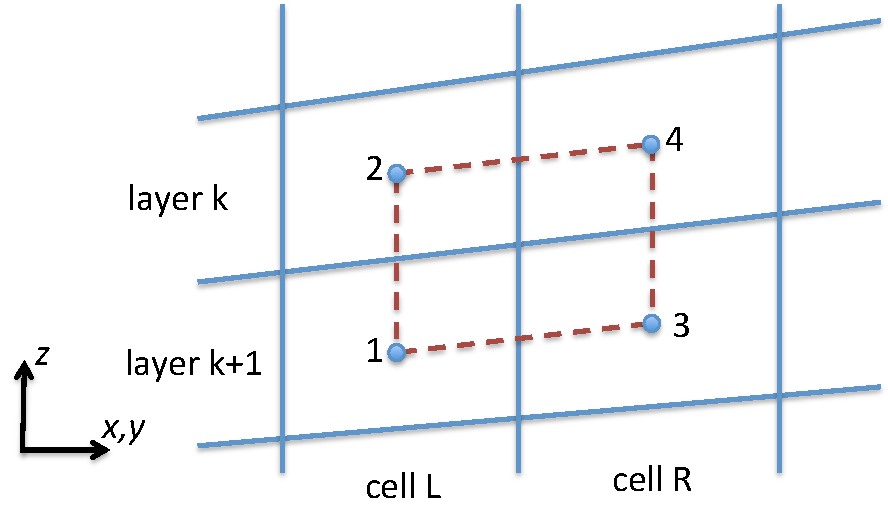
\includegraphics[width=3.5in]{ocean/figures/common_level.pdf}
\caption{Vertical cross-section of ocean grid cells, showing index locations for common level method.  The dots are placed at cell centers in the horizontal and layer mid-depth in the vertical.}
\label{oceanFigure:common level}
\end{figure}

{\bf \large config\_pressure\_gradient\_type = 'Jacobian\_from\_density'}\\
In this formulation the pressure gradient is rewritten in terms of a sea surface height gradient and the vertical integral of a Jacobian,
\begin{eqnarray}
\label{ocean:grad p Jacobian}
- \frac{1}{\rho_0}\nabla_z p &=& - \frac{\rho_s g}{\rho_0}\nabla_s \zeta - \frac{g}{\rho_0}\int_z^\zeta {\mathcal J}(\rho,z)ds, \\
{\mathcal J}(\rho,z) &=& \left. \frac{\partial \rho}{\partial x} \right|_s \frac{\partial z}{\partial s} 
 - \frac{\partial \rho}{\partial s}  \left. \frac{\partial z}{\partial x} \right|_s 
\end{eqnarray}
where $x$ is a general horizontal direction between two cell centers and $s$ is the vertical coordinate reference, i.e.\ $s$ is constant within a layer.  There are many methods to discretize the Jacobian term.  In the common level method, the density is linearly interpolated or extrapolated within each vertical column to a common level $z_\gamma$ (see Figure \ref{oceanFigure:common level}):
\begin{eqnarray}
- \int_z^\zeta {\mathcal J}(\rho,z)ds &=& \overline{\Delta z} \left( \rho^L - \rho^R \right) \\
\overline{\Delta z} &=& \frac{1}{2} \left(z_2-z_1 + z_4-z_3\right) \\
\rho^L &=& \frac{\rho_1\left(z_2-z_\gamma\right) + \rho_2\left(z_\gamma-z_1\right) }{z_2-z_1}\\
\rho^R &=& \frac{\rho_3\left(z_4-z_\gamma\right) + \rho_4\left(z_\gamma-z_3\right) }{z_4-z_3}\\
z_\gamma &=& \left(1-\gamma\right)z_* + \gamma z_c \\
z_* &=&  \frac{z_4 z_2-z_3z_1}{z_4-z_3 + z_2-z_1} \\
z_c &=&  \frac{z_1+z_2+z_3+z_4}{4} 
\end{eqnarray}
where $z_c$ is the depth for the weighted Jacobian method by \citet{Song98mwr}, and $z_*$ is the depth for the standard Jacobian method, which is the depth of intersection of the diagonals of the trapezoidal element in Figure \ref{oceanFigure:common level}.  Here $\gamma$ weights the choice between these two methods for computing the common level $z_\gamma$.  This formulation for the pressure gradient is described in detail in \citet{Shchepetkin_McWilliams03jgr}, Section 2, method 2, and Section 4.  They found that a coefficient of $\gamma=0.5$, which gives equal weights to the standard and weighted Jacobian methods, minimizes the errors in a seamount test problem.

{\bf \large config\_pressure\_gradient\_type = 'Jacobian\_from\_TS'}\\
This formulation is the same as the previous, except that the Jacobian is computed using a linear expansion in potential temperature and salinity.  This option must be used when layers are extremely tilted, such as with sigma coordinates or under an ice shelf, in combination with a nonlinear equation of state.
\begin{eqnarray}
 {\mathcal J}(\rho,z) &=& -\alpha  {\mathcal J}(\theta,z) + \beta  {\mathcal J}(S,z), 
\end{eqnarray}
where
\begin{eqnarray}
\alpha\left( \theta, S, p\right) &=&  -\left. \frac{\partial \rho}{\partial \theta} \right|_{S,p} \\
\beta\left( \theta, S, p\right) &=&  \left. \frac{\partial \rho}{\partial S} \right|_{\theta,p} 
\end{eqnarray}
are the thermal expansion and saline contraction coefficients, computed at a particular  $\left(\theta, S, p\right)$ by the equation of state \citep[eqn 7.16]{Shchepetkin_McWilliams03jgr}.

{\bf \large config\_pressure\_gradient\_type = 'MontgomeryPotential'}\\
For isopycnal vertical coordinates, the user may choose to use the Montgomery potential,
\begin{equation}
\label{ocean:Montgomery Potential}
M = \frac{1}{\rho}p+gz
\end{equation}
and replace the pressure terms above with
\begin{equation}
- \nabla_s M.
\end{equation}
See \citet[section 2.1]{Higdon05jcp} for details on the derivation and computation of the Montgomery potential.

% {\bf \large config\_pressure\_gradient\_type = 'MontgomeryPotential\_and\_density'}
% Same as previous, but this formulation includes an extra term,
% \begin{equation}
% - \nabla_s M + p \nabla_s\left(\frac{1}{\rho} \right),
% \end{equation}
% as described by \citet{Bleck02om}, eqn 1 and end of Appendix A.  This formulation has not been extensively tested and is not supported at this time.

\vspace{0.5in}
{\small
\begin{center}
\begin{longtable}{| p{2.0in} || p{4.0in} |}
    \hline
    {\bf Name} & {\bf Description} \endfirsthead
    \hline 
    {\bf Name} & {\bf Description} (Continued) \endhead
    \hline
    \hline
    \hyperref[subsec:nm_sec_config_pressure_gradient_type]{config\_pressure\_gradient\_type} & Form of pressure gradient terms in momentum equation. For most applications, the gradient of pressure and layer mid-depth are appropriate.  For isopycnal coordinates, one may use the gradient of the Montgomery potential.  The sea surface height gradient (ssh\_gradient) option is for barotropic, depth-averaged pressure. \\
    \hline
    \hyperref[subsec:nm_sec_config_common_level_weight]{config\_common\_level\_weight} & The weight between standard Jacobian and weighted Jacobian, $\gamma$. \\
    \hline
    \hyperref[subsec:nm_sec_config_zonal_ssh_grad]{config\_zonal\_ssh\_grad} & The zonal (x) ssh gradient to be applied. \\
    \hline
    \hyperref[subsec:nm_sec_config_meridional_ssh_grad]{config\_meridional\_ssh\_grad} & The meridional (y) ssh gradient to be applied. \\
    \hline
\end{longtable}
\end{center}
}
\section[eos]{\hyperref[sec:nm_sec_eos]{eos}}
\label{sec:nm_tab_eos}
Two forms of EOS are supported. The full EOS from \cite{Jackett_McDougall95jaot} and a linear EOS.

\vspace{0.5in}
{\small
\begin{center}
\begin{longtable}{| p{2.0in} || p{4.0in} |}
    \hline
    {\bf Name} & {\bf Description} \endfirsthead
    \hline 
    {\bf Name} & {\bf Description} (Continued) \endhead
    \hline
    \hline
    \hyperref[subsec:nm_sec_config_eos_type]{config\_eos\_type} & Character string to choose EOS formulation \\
    \hline
    \hyperref[subsec:nm_sec_config_open_ocean_freezing_temperature_coeff_0]{config\_open\_ocean\_freezing\_\-temperature\_coeff\_0} & The freezing temperature at zero pressure and salinity in open ocean. \\
    \hline
    \hyperref[subsec:nm_sec_config_open_ocean_freezing_temperature_coeff_S]{config\_open\_ocean\_freezing\_\-temperature\_coeff\_S} & The coefficient for the term proportional to salinity in the freezing temperature in the open ocean. \\
    \hline
    \hyperref[subsec:nm_sec_config_open_ocean_freezing_temperature_coeff_p]{config\_open\_ocean\_freezing\_\-temperature\_coeff\_p} & The coefficient for the term proportional to the pressure in the freezing temperature in the open ocean. \\
    \hline
    \hyperref[subsec:nm_sec_config_open_ocean_freezing_temperature_coeff_pS]{config\_open\_ocean\_freezing\_\-temperature\_coeff\_pS} & The coefficient for the term proportional to salinity times pressure in the freezing temperature in the open ocean. \\
    \hline
    \hyperref[subsec:nm_sec_config_open_ocean_freezing_temperature_coeff_mushy_az1_liq]{config\_open\_ocean\_freezing\_\-temperature\_coeff\_mushy\_az1\_\-liq} & The coefficient for the mushy sea-ice physics term az1\_liq in the open ocean. \\
    \hline
    \hyperref[subsec:nm_sec_config_land_ice_cavity_freezing_temperature_coeff_0]{config\_land\_ice\_cavity\_\-freezing\_temperature\_coeff\_0} & The freezing temperature at zero pressure and salinity in land-ice cavities. \\
    \hline
    \hyperref[subsec:nm_sec_config_land_ice_cavity_freezing_temperature_coeff_S]{config\_land\_ice\_cavity\_\-freezing\_temperature\_coeff\_S} & The coefficient for the term proportional to salinity in the freezing temperature in land-ice cavities. \\
    \hline
    \hyperref[subsec:nm_sec_config_land_ice_cavity_freezing_temperature_coeff_p]{config\_land\_ice\_cavity\_\-freezing\_temperature\_coeff\_p} & The coefficient for the term proportional to the pressure in the freezing temperature in land-ice cavities. \\
    \hline
    \hyperref[subsec:nm_sec_config_land_ice_cavity_freezing_temperature_coeff_pS]{config\_land\_ice\_cavity\_\-freezing\_temperature\_coeff\_pS} & The coefficient for the term proportional to salinity times pressure in the freezing temperature in land-ice cavities. \\
    \hline
\end{longtable}
\end{center}
}
\section[eos\_linear]{\hyperref[sec:nm_sec_eos_linear]{eos\_linear}}
\label{sec:nm_tab_eos_linear}
The linear equation of state (leos) is specified as follows:
\begin{equation}
\rho = \rho_{ref} - \alpha_{leos}(T-T_{ref})+\beta_{leos}(S-S_{ref})
\end{equation}
\vspace{0.5in}
{\small
\begin{center}
\begin{longtable}{| p{2.0in} || p{4.0in} |}
    \hline
    {\bf Name} & {\bf Description} \endfirsthead
    \hline 
    {\bf Name} & {\bf Description} (Continued) \endhead
    \hline
    \hline
    \hyperref[subsec:nm_sec_config_eos_linear_alpha]{config\_eos\_linear\_alpha} & Linear thermal expansion coefficient \\
    \hline
    \hyperref[subsec:nm_sec_config_eos_linear_beta]{config\_eos\_linear\_beta} & Linear haline contraction coefficient \\
    \hline
    \hyperref[subsec:nm_sec_config_eos_linear_Tref]{config\_eos\_linear\_Tref} & Reference temperature \\
    \hline
    \hyperref[subsec:nm_sec_config_eos_linear_Sref]{config\_eos\_linear\_Sref} & Reference salinity \\
    \hline
    \hyperref[subsec:nm_sec_config_eos_linear_densityref]{config\_eos\_linear\_densityref} & Reference density, i.e. density when T=Tref and S=Sref \\
    \hline
\end{longtable}
\end{center}
}
\section[eos\_wright]{\hyperref[sec:nm_sec_eos_wright]{eos\_wright}}
\label{sec:nm_tab_eos_wright}
\vspace{0.5in}
{\small
\begin{center}
\begin{longtable}{| p{2.0in} || p{4.0in} |}
    \hline
    {\bf Name} & {\bf Description} \endfirsthead
    \hline 
    {\bf Name} & {\bf Description} (Continued) \endhead
    \hline
    \hline
    \hyperref[subsec:nm_sec_config_eos_wright_ref_pressure]{config\_eos\_wright\_ref\_pressure} & Reference pressure for potential density \\
    \hline
\end{longtable}
\end{center}
}
\section[split\_timestep\_share]{\hyperref[sec:nm_sec_split_timestep_share]{split\_timestep\_share}}
\label{sec:nm_tab_split_timestep_share}
\vspace{0.5in}
{\small
\begin{center}
\begin{longtable}{| p{2.0in} || p{4.0in} |}
    \hline
    {\bf Name} & {\bf Description} \endfirsthead
    \hline 
    {\bf Name} & {\bf Description} (Continued) \endhead
    \hline
    \hline
    \hyperref[subsec:nm_sec_config_n_ts_iter]{config\_n\_ts\_iter} & number of large iterations over stages 1-3; For the split\_explicit\_ab2 time integrator, this value only affects the first time step when it is not a restart run. For restart runs, this value has no effect on the split\_explicit\_ab2 time integrator. \\
    \hline
    \hyperref[subsec:nm_sec_config_n_bcl_iter_beg]{config\_n\_bcl\_iter\_beg} & number of iterations of stage 1 (baroclinic solve) on the first split timestepping iteration \\
    \hline
    \hyperref[subsec:nm_sec_config_n_bcl_iter_mid]{config\_n\_bcl\_iter\_mid} & number of iterations of stage 1 (baroclinic solve) on any split timestepping iterations between first and last \\
    \hline
    \hyperref[subsec:nm_sec_config_n_bcl_iter_end]{config\_n\_bcl\_iter\_end} & number of iterations of stage 1 (baroclinic solve) on the last split timestepping iteration \\
    \hline
\end{longtable}
\end{center}
}
\section[split\_explicit\_ts]{\hyperref[sec:nm_sec_split_explicit_ts]{split\_explicit\_ts}}
\label{sec:nm_tab_split_explicit_ts}
The split explicit time-stepping method solves the barotropic (vertically-integrated) velocities separately from the remaining baroclinic velocities.  The time step for the barotropic solve is limited by fast surface gravity waves, and so is subcycled within a large timestep of the baroclinic velocity solve.  This provides a 10 to 12-times speed-up over fourth-order Runge-Kutta time stepping.

A single large timestep in the split explicit algorithm may be summarized as
\begin{itemize}
\item Stage 1: solve for baroclinic velocity (3D)
\item Stage 2: solve for barotropic velocity (2D) with explicit sub-cycling
\item Stage 3: update thickness, tracers, density and pressure
\end{itemize}
The algorithm includes iterations within stage 1, within each subcycle of stage 2, and over the full three-stage process.  Further details are provided in \citet[Appendix A.5]{Ringler_ea13om}

\vspace{0.5in}
{\small
\begin{center}
\begin{longtable}{| p{2.0in} || p{4.0in} |}
    \hline
    {\bf Name} & {\bf Description} \endfirsthead
    \hline 
    {\bf Name} & {\bf Description} (Continued) \endhead
    \hline
    \hline
    \hyperref[subsec:nm_sec_config_btr_dt]{config\_btr\_dt} & Timestep to use for the barotropic mode in the split explicit time integrator \\
    \hline
    \hyperref[subsec:nm_sec_config_n_btr_cor_iter]{config\_n\_btr\_cor\_iter} & number of iterations of the velocity corrector step in stage 2 \\
    \hline
    \hyperref[subsec:nm_sec_config_vel_correction]{config\_vel\_correction} & If true, the velocity correction term is included in the horizontal advection of thickness and tracers \\
    \hline
    \hyperref[subsec:nm_sec_config_btr_subcycle_loop_factor]{config\_btr\_subcycle\_loop\_\-factor} & Barotropic subcycles proceed from $t$ to $t+n\Delta t$, where $n$ is this configuration option. \\
    \hline
    \hyperref[subsec:nm_sec_config_btr_gam1_velWt1]{config\_btr\_gam1\_velWt1} & Weighting of velocity in the SSH predictor step in stage 2. When zero, previous subcycle time is used; when one, new subcycle time is used. \\
    \hline
    \hyperref[subsec:nm_sec_config_btr_gam2_SSHWt1]{config\_btr\_gam2\_SSHWt1} & Weighting of SSH in the velocity corrector step in stage 2. When zero, previous subcycle time is used; when one, new subcycle time is used. \\
    \hline
    \hyperref[subsec:nm_sec_config_btr_gam3_velWt2]{config\_btr\_gam3\_velWt2} & Weighting of velocity in the SSH corrector step in stage 2. When zero, previous subcycle time is used; when one, new subcycle time is used. \\
    \hline
    \hyperref[subsec:nm_sec_config_btr_solve_SSH2]{config\_btr\_solve\_SSH2} & If true, execute the SSH corrector step in stage 2 \\
    \hline
\end{longtable}
\end{center}
}
\section[split\_implicit\_ts]{\hyperref[sec:nm_sec_split_implicit_ts]{split\_implicit\_ts}}
\label{sec:nm_tab_split_implicit_ts}
\vspace{0.5in}
{\small
\begin{center}
\begin{longtable}{| p{2.0in} || p{4.0in} |}
    \hline
    {\bf Name} & {\bf Description} \endfirsthead
    \hline 
    {\bf Name} & {\bf Description} (Continued) \endhead
    \hline
    \hline
    \hyperref[subsec:nm_sec_config_btr_si_preconditioner]{config\_btr\_si\_preconditioner} & Type of preconditioner for the barotropic mode solver \\
    \hline
    \hyperref[subsec:nm_sec_config_btr_si_tolerance]{config\_btr\_si\_tolerance} & Tolerance for the barotropic mode solver \\
    \hline
    \hyperref[subsec:nm_sec_config_n_btr_si_large_iter]{config\_n\_btr\_si\_large\_iter} & number of large barotropic system iterations \\
    \hline
    \hyperref[subsec:nm_sec_config_btr_si_partition_match_mode]{config\_btr\_si\_partition\_\-match\_mode} & If true, the split-implicit method uses the Jacobi preconditioner with the bit-for-bit all-reduce. This is less performant, so should only be used for testing. \\
    \hline
\end{longtable}
\end{center}
}
\section[ALE\_vertical\_grid]{\hyperref[sec:nm_sec_ALE_vertical_grid]{ALE\_vertical\_grid}}
\label{sec:nm_tab_ALE_vertical_grid}
The MPAS-Ocean vertical grid is structured arbitrary Lagrangian-Eulerian (ALE).   ALE provides a great deal of freedom in the choice of vertical coordinate: when fully Eulerian, MPAS-Ocean is a z-level model with fixed thicknesses; when fully Lagrangian, there is no vertical transport between layers, and layers expand and contract like an isopycnal ocean model.  In between are many additional options, such as z-star where layers expand in proportion to the sea surface height, and sigma, where coordinates are terrain-following.

MPAS-Ocean employs the continuity equation,
\begin{eqnarray}
\label{ocean:continuity thickness}
\frac{\partial h_{k}}{\partial t} + D_k + w^t_k - w^t_{k+1} =0
\end{eqnarray}
for the ALE formulation, where variables are defined in Table \ref{oceanTable:ALE_variables}.  The ALE algorithm is as follows:
\begin{enumerate}
\item ALE step: Compute desired thickness for the new time,
\begin{eqnarray}
\label{ocean:desired thickness}
h_k^{ALE} = h_k^{rest} + h_k^{SSH} + h_k^{hf} + h_k^{min}
\end{eqnarray}
\item ALE step: Solve for vertical transport $w^t$ from (\ref{ocean:continuity thickness}),
\begin{eqnarray}
\label{ocean:vert tranport}
w^t_k = w^t_{k+1} - D_k - \frac{h^{ALE}_k - h^n_k}{\Delta t}
\end{eqnarray}
\item Solve for new thickness, $h_{k}^{n+1}$, using the continuity equation (\ref{ocean:continuity thickness}) within the time integration routine.
\end{enumerate}
The redundancy in steps 2 and 3 are intentional, so that step 2 is isolated within the ALE subroutine, and step 3 is solved in the timestepping subroutine in the identical manner as the tracer equation (\ref{ocean:tracer}).

The desired ALE thickness includes contributions from four terms (\ref{ocean:desired thickness}):
\begin{enumerate}
\item {\bf Resting thickness}, $h^{rest}$, is the layer thickness when the ocean is at rest, i.e. without SSH or internal perturbations.  For z-type coordinates, the resting thickness is constant in each horizontal layer.
\item {\bf SSH alteration}, $h^{SSH}$, alters layer thicknesses so that they change in proportion to the sea surface height (SSH),
\begin{eqnarray}
\label{ocean:h ssh}
   h_k^{SSH} =  \zeta \frac{W_k h^{rest}_k}{\sum_{k'=1}^{kmax}W_{k'}h^{rest}_{k'}}
\end{eqnarray}
The weights $W_k$ determine how SSH oscillations are distributed amongst the layers, as described in Table \ref{oceanTable:vertical coordinates}.
\item {\bf High-frequency thickness}, $h^{hf}$, allows high-frequency thickness oscillations, such as internal gravity waves, to be treated in a Lagrangian manner.  This is the ``z-tilde'' scheme of \citet{Leclair_Madec11om} described in the next section.
\item {\bf Minimum thickness alteration}, $h^{min}$, is the change in thickness required to enforce the minimum thickness in each cell.  When a cell is too thin, $h^{min}$ is positive, while nearby cells in the vertical incur a corresponding negative $h^{min}$ to conserve volume in the column.
\end{enumerate}
Of the four terms, resting thickness is always positive, while the others are small alterations about zero.  Summing a column,
\begin{eqnarray}
\sum_{k=1}^{kmax} h_k^{ALE} &=& \sum_{k=1}^{kmax} h_k^{rest} + \sum_{k=1}^{kmax}h_k^{SSH} + \sum_{k=1}^{kmax}h_k^{hf} + \sum_{k=1}^{kmax}h_k^{min} 
\nonumber \\
&=& H + \zeta + 0 + 0.
\nonumber
\end{eqnarray}
Thus the first two terms are always included so that the column thickness sums to $H+\zeta$, while the second two terms are optional and may be turned on with flags.

In order to assist users in choosing the correct settings, we provide a description of traditional vertical coordinate names in Table \ref{oceanTable:vertical coordinates}.
The vertical coordinate type also depends upon the set-up of the layerThickness variable in the initial condition file.  For all Z-type vertical coordinates, initial layer thicknesses are horizontally constant.  For sigma coordinates, layers are terrain-following and all layers are employed.  In this case, the user may still choose amongst the flags in SSH may be distributed through the column just like with z-type models in Table \ref{oceanTable:vertical coordinates}.

In order to run an isopycnal configuration, use config\_vert\_coord\_movement='impermeable\_interfaces' and set initial temperature and salinity to be constant within each layer.  All vertical tracer diffusion must be off so that the density in each layer remains constant.  For an isopycnal set-up, the equation of state is still called at each timestep, so a linear equation of state is recommended to avoid depth-dependancy of the density.  The user may choose a Montgomery Potential (\ref{ocean:Montgomery Potential}) or standard pressure gradient (\ref{ocean:grad p}); Montgomery Potential is a more common choice for isopycnal configurations, but both are tested and functional.  MPAS-Ocean does not support massless layers at this time, so isopycnal vertical coordinates may only be used for idealized domains.

\begin{table}[ht] 
\caption{Vertical coordinate settings for traditional names.}
\vspace{0.5cm} \centering 
\begin{tabular}{c c c c c c} 
\hline\hline flag name &  {\bf Z-Level} & {\bf Z-star} & {\bf weighted Z-star} &  {\bf isopycnal}  \\
\hline 
config\_vert\_ & 'fixed' & 'uniform\_stretching' & 'user\_specified' & 'impermeable\_ \\
coord\_movement & & & & interfaces'
\\
weights & $W_k =\left\{ \begin{array}{c} 1\; k=1\\ 0\; k>1 \end{array}\right.$ & $W_k=1\;\;\forall\;\;k$ & input file & not applicable \\
\hline 
\end{tabular} \label{oceanTable:vertical coordinates} 
\end{table}

\begin{table}[h!t] 
\caption{Variables used in ALE equation sets.  Column 3 shows the native horizontal grid location.  A subscript $k$ indicates indicates the layer index.  The $\nabla$ indicates a horizontal gradient within a single layer.} 
\vspace{0.5cm} \centering 
\begin{tabular}{c c c c } 
\hline\hline symbol &  name & grid &  notes  \\
\hline 
$D$  & thickness-weighted divergence & cell & $D_k = \nabla \cdot  \left( h_k {\bf u}_k \right)$  \\ 
${\bar D}$ & barotropic divergence & cell & ${\overline D} = \sum\limits_{k=1}^{kmax} D_k$  \\ 
$D'$  & baroclinic divergence & cell & $D'_k = D_k-\frac{h_k}{H}{\bar D}$  \\ 
$D^{lf}$  & low-frequency divergence & cell & see (\ref{ocean:Dlf})  \\ 
$D^{hf}$  & high-frequency divergence & cell & $D^{hf}_k = D'_k - D^{lf}_k$  \\ 
$h$  & layer thickness & cell &   \\ 
$h^{ALE}$  & desired ALE thickness & cell & see (\ref{ocean:desired thickness})  \\ 
$h^{rest}$  & resting thickness & cell &   \\ 
$h^{SSH}$  & SSH thickness alteration & cell & see (\ref{ocean:h ssh})  \\ 
$h^{hf}$  & high-freq. thickness alteration & cell &   see (\ref{ocean:hhf})  \\ 
$h^{min}$  & minimum thickness alteration & cell &   \\ 
$H$  & total resting thickness & cell & $H= \sum\limits_{k=1}^{kmax} h_k^{rest}$  \\ 
${\bf u}$  & velocity & edge &   \\ 
$w^t$ & vertical transport & cell  & top of layer in vertical \\
$W$  & SSH thickness weights & cell &   \\ 
$\tau_{Dlf}$  & frequency filter time scale & constant &   \\ 
$\tau_{hhf}$  & restoring time scale for $h^{hf}$ & constant &   \\ 
$\kappa_{hhf}$  & $h^{hf}$ diffusion & constant &   \\ 
$\zeta$  & sea surface height & cell &  $\zeta= \sum\limits_{k=1}^{kmax} h_k^{rest} - H$  \\ 
\hline 
\end{tabular} \label{oceanTable:ALE_variables} 
\end{table}


\vspace{0.5in}
{\small
\begin{center}
\begin{longtable}{| p{2.0in} || p{4.0in} |}
    \hline
    {\bf Name} & {\bf Description} \endfirsthead
    \hline 
    {\bf Name} & {\bf Description} (Continued) \endhead
    \hline
    \hline
    \hyperref[subsec:nm_sec_config_vert_coord_movement]{config\_vert\_coord\_movement} & Determines the vertical coordinate movement type. 'uniform\_stretching' distributes SSH perturbations through all vertical levels (z-star vertical coordinate); 'fixed' places them all in the top level (z-level vertical coordinate); 'user\_specified' allows the input file to determine the distribution using the variable vertCoordMovementWeights (weighted z-star vertical coordinate); and 'impermeable\_interfaces' makes the vertical transport between layers zero, i.e. $w^t=0$ (idealized isopycnal). \\
    \hline
    \hyperref[subsec:nm_sec_config_ALE_thickness_proportionality]{config\_ALE\_thickness\_\-proportionality} & When config\_vert\_coord\_movement='uniform\_stretching' (z-star type coordinate), determines whether ALE layer thickness is proportional to the resting thickness times weights, or just the weights. The first is standard for global runs and is what is specified in Petersen et al 2015 eqns 4 and 6. The second is useful for wetting/drying test cases where resting thickness may be zero at the coastlines. \\
    \hline
    \hyperref[subsec:nm_sec_config_vert_taper_weight_depth_1]{config\_vert\_taper\_weight\_\-depth\_1} & Vertical coordinate taper weight is one above this depth, linearly decreases to zero below. \\
    \hline
    \hyperref[subsec:nm_sec_config_vert_taper_weight_depth_2]{config\_vert\_taper\_weight\_\-depth\_2} & Vertical coordinate taper weight is zero below this depth, linearly increases to one above. \\
    \hline
    \hyperref[subsec:nm_sec_config_use_min_max_thickness]{config\_use\_min\_max\_thickness} & If true, a minimum and maximum thicknesses are enforced to prevent massless and very thick layers. \\
    \hline
    \hyperref[subsec:nm_sec_config_min_thickness]{config\_min\_thickness} & Minimum thickness allowed. \\
    \hline
    \hyperref[subsec:nm_sec_config_max_thickness_factor]{config\_max\_thickness\_factor} & Maximum thickness allowed. This is a factor times the resting thickness, i.e., maximum thickness = config\_max\_thickness\_factor*$h^{rest}$. \\
    \hline
    \hyperref[subsec:nm_sec_config_dzdk_positive]{config\_dzdk\_positive} & Determines if the positive Z axis is aligned with the positive K index direction. \\
    \hline
\end{longtable}
\end{center}
}
\section[ALE\_frequency\_filtered\_thickness]{\hyperref[sec:nm_sec_ALE_frequency_filtered_thickness]{ALE\_frequency\_filtered\_thickness}}
\label{sec:nm_tab_ALE_frequency_filtered_thickness}
The high-frequency thickness alteration, $h^{hf}$, in (\ref{ocean:\mode_desired thickness}) allows the thicknesses to oscillate so that high-frequency motions, such as internal gravity waves, are treated in a Lagrangian manner.  Low-freqency motions, such as seasonal changes or slow motions of water masses, are treated in an Eulerian manner.  This is the ``z-tilde'' scheme of \citet{Leclair_Madec11om}, which generally reduces spurious vertical mixing and preserves water mass properties.  Two additional prognostic equations are solved when config\_use\_freq\_filtered\_thickness is true,
\begin{eqnarray}
\label{ocean:\mode_Dlf}
 & \displaystyle
  \frac{\partial D^{lf}_k}{\partial t} = - \frac{2\pi}{\tau_{Dlf}} \left( D^{lf}_k - D'_k \right), 
\\ & \displaystyle
\label{ocean:\mode_hhf}
\frac{\partial h^{hf}_k}{\partial t} =  - D^{hf}_k - \frac{2\pi}{\tau_{hhf}} h^{hf}_k + \nabla_h\cdot \left( \kappa_{hhf} \nabla_h h^{hf}_k \right) 
\end{eqnarray}
where $\tau_{Dlf}$ is the filter timescale and other variables are defined in Table \ref{oceanTable:\mode_ALE_variables}.  This may be used in addition to any of the z-type or sigma-type vertical coordinates in Table \ref{oceanTable:\mode_vertical coordinates}.  Some combination of thickness restoring and diffusion are recommended to avoid long-term drift of $h^{hf}$ away from zero.




\vspace{0.5in}
{\small
\begin{center}
\begin{longtable}{| p{2.0in} || p{4.0in} |}
    \hline
    {\bf Name} & {\bf Description} \endfirsthead
    \hline 
    {\bf Name} & {\bf Description} (Continued) \endhead
    \hline
    \hline
    \hyperref[subsec:nm_sec_config_use_freq_filtered_thickness]{config\_use\_freq\_filtered\_\-thickness} & If true, $h^{hf}$ is included in the desired ALE thickness, and the prognostic equations for $D^{lf}$ and $h^{hf}$ are integrated in the code. \\
    \hline
    \hyperref[subsec:nm_sec_config_thickness_filter_timescale]{config\_thickness\_filter\_timescale} & Filter time scale for the low-frequency baroclinic divergence, $\tau_{Dlf}$. \\
    \hline
    \hyperref[subsec:nm_sec_config_use_highFreqThick_restore]{config\_use\_highFreqThick\_\-restore} & If true, the high frequency thickness prognostic equation ($h^{hf}$) includes term 2 on the RHS, the restoring term.  The high frequency thickness is restored to zero with time scale $\tau_{hhf}$. \\
    \hline
    \hyperref[subsec:nm_sec_config_highFreqThick_restore_time]{config\_highFreqThick\_restore\_\-time} & Restoring time scale for high-frequency thickness, $\tau_{hhf}$. \\
    \hline
    \hyperref[subsec:nm_sec_config_use_highFreqThick_del2]{config\_use\_highFreqThick\_del2} & If true, high frequency thickness prognostic equation ($h^{hf}$) includes term 3 on the RHS, the diffusion term. \\
    \hline
    \hyperref[subsec:nm_sec_config_highFreqThick_del2]{config\_highFreqThick\_del2} & Horizontal high frequency thickness diffusion, $\kappa_{hhf}$. \\
    \hline
\end{longtable}
\end{center}
}
\section[debug]{\hyperref[sec:nm_sec_debug]{debug}}
\label{sec:nm_tab_debug}
At run-time a user can enable debugging features within MPAS-Ocean. These
features include disabling any tendencies to help determine why an issue might
be happening. Debugging options also include various checks on certain fields,
and the ability to prescribe both a thickness and velocity field at run-time
which are constant throughout a simulation. All options that control these
debugging features are specified within the debug namelist record.

\vspace{0.5in}
{\small
\begin{center}
\begin{longtable}{| p{2.0in} || p{4.0in} |}
    \hline
    {\bf Name} & {\bf Description} \endfirsthead
    \hline 
    {\bf Name} & {\bf Description} (Continued) \endhead
    \hline
    \hline
    \hyperref[subsec:nm_sec_config_check_zlevel_consistency]{config\_check\_zlevel\_consistency} & Enables a run-time check for consistency for a zlevel grid. Ensures relevant variables correctly define the bottom of the ocean. \\
    \hline
    \hyperref[subsec:nm_sec_config_check_ssh_consistency]{config\_check\_ssh\_consistency} & Enables a run-time check to determine if the SSH is within 2m of the surface.  See equation for $\zeta_i$. \\
    \hline
    \hyperref[subsec:nm_sec_config_filter_btr_mode]{config\_filter\_btr\_mode} & Enables filtering of the barotropic mode. \\
    \hline
    \hyperref[subsec:nm_sec_config_prescribe_velocity]{config\_prescribe\_velocity} & Enables a prescribed velocity field. This velocity field is read on input, and remains constant through a simulation. \\
    \hline
    \hyperref[subsec:nm_sec_config_prescribe_thickness]{config\_prescribe\_thickness} & Enables a prescribed thickness field. This thickness field is read on input, and remains constant through a simulation. \\
    \hline
    \hyperref[subsec:nm_sec_config_include_KE_vertex]{config\_include\_KE\_vertex} & If true, the kinetic energy in each cell is computed by blending cell-based and vertex-based values of kinetic energy. \\
    \hline
    \hyperref[subsec:nm_sec_config_check_tracer_monotonicity]{config\_check\_tracer\_\-monotonicity} & Enables a change on tracer monotonicity at the end of the monotonic advection routine. Only used if config\_flux\_limiter is set to monotonic \\
    \hline
    \hyperref[subsec:nm_sec_config_compute_active_tracer_budgets]{config\_compute\_active\_tracer\_\-budgets} & Enables the computation of tracer budget terms \\
    \hline
    \hyperref[subsec:nm_sec_config_disable_thick_all_tend]{config\_disable\_thick\_all\_tend} & Disables all tendencies on the thickness field. \\
    \hline
    \hyperref[subsec:nm_sec_config_disable_thick_hadv]{config\_disable\_thick\_hadv} & Disable tendencies on the thickness field from horizontal advection. \\
    \hline
    \hyperref[subsec:nm_sec_config_disable_thick_vadv]{config\_disable\_thick\_vadv} & Disables tendencies on the thickness field from vertical advection. \\
    \hline
    \hyperref[subsec:nm_sec_config_disable_thick_sflux]{config\_disable\_thick\_sflux} & Disables tendencies on the thickness field from surface fluxes. \\
    \hline
    \hyperref[subsec:nm_sec_config_disable_vel_all_tend]{config\_disable\_vel\_all\_tend} & Disables all tendencies on the velocity field. \\
    \hline
    \hyperref[subsec:nm_sec_config_disable_vel_hadv]{config\_disable\_vel\_hadv} & Disables tendencies on the velocity field from the horizontal momentum advection. Note that these two flags are set together for linearized test cases: config\_thickness\_flux\_type = 'constant' linearizes the thickness equation, and config\_disable\_vel\_hadv = .true. linearizes the momentum equation if there is no assumed mean background velocity. \\
    \hline
    \hyperref[subsec:nm_sec_config_disable_vel_coriolis]{config\_disable\_vel\_coriolis} & Disables tendencies on the velocity field from the Coriolis force. \\
    \hline
    \hyperref[subsec:nm_sec_config_disable_vel_pgrad]{config\_disable\_vel\_pgrad} & Disables tendencies on the velocity field from the horizontal pressure gradient. \\
    \hline
    \hyperref[subsec:nm_sec_config_disable_vel_hmix]{config\_disable\_vel\_hmix} & Disables tendencies on the velocity field from horizontal mixing. \\
    \hline
    \hyperref[subsec:nm_sec_config_disable_vel_surface_stress]{config\_disable\_vel\_surface\_\-stress} & Disables tendencies on the velocity field from horizontal surface stresses (e.g. wind stress and top drag). \\
    \hline
    \hyperref[subsec:nm_sec_config_disable_vel_topographic_wave_drag]{config\_disable\_vel\_\-topographic\_wave\_drag} & Disables tendencies on the velocity field from topographic wave drag \\
    \hline
    \hyperref[subsec:nm_sec_config_disable_vel_explicit_bottom_drag]{config\_disable\_vel\_explicit\_\-bottom\_drag} & Disables tendencies on the velocity field from explicit bottom drag \\
    \hline
    \hyperref[subsec:nm_sec_config_disable_vel_vmix]{config\_disable\_vel\_vmix} & Disables tendencies on the velocity field from vertical mixing. \\
    \hline
    \hyperref[subsec:nm_sec_config_disable_vel_vadv]{config\_disable\_vel\_vadv} & Disables tendencies on the velocity field from vertical advection. \\
    \hline
    \hyperref[subsec:nm_sec_config_disable_tr_all_tend]{config\_disable\_tr\_all\_tend} & Disables all tendencies on tracer fields. \\
    \hline
    \hyperref[subsec:nm_sec_config_disable_tr_adv]{config\_disable\_tr\_adv} & Disables tendencies on tracer fields from advection, both horizontal and vertical. \\
    \hline
    \hyperref[subsec:nm_sec_config_disable_tr_hmix]{config\_disable\_tr\_hmix} & Disables tendencies on tracer fields from horizontal mixing. \\
    \hline
    \hyperref[subsec:nm_sec_config_disable_tr_vmix]{config\_disable\_tr\_vmix} & Disables tendencies on tracer fields from vertical mixing. \\
    \hline
    \hyperref[subsec:nm_sec_config_disable_tr_sflux]{config\_disable\_tr\_sflux} & Disables tendencies on tracer fields from surface fluxes. \\
    \hline
    \hyperref[subsec:nm_sec_config_disable_tr_nonlocalflux]{config\_disable\_tr\_nonlocalflux} & Disables tendencies on the tracer fields from CVMix/KPP nonlocal fluxes. \\
    \hline
    \hyperref[subsec:nm_sec_config_disable_redi_k33]{config\_disable\_redi\_k33} & If true, disables k33 portion of Redi neutral surface mixing. \\
    \hline
    \hyperref[subsec:nm_sec_config_read_nearest_restart]{config\_read\_nearest\_restart} & This flag is intended for the expert user.  If false, forward model will error out if time given by config\_start\_time (or Restart\_timestamp file if config\_start\_time='file') does not match any xtime strings in the restart file.  If true, forward model will read in record with xtime nearest to config\_start\_time.  Note that the restart file name is still given by config\_start\_time (or Restart\_timestamp file), regardless of the state of this flag. \\
    \hline
\end{longtable}
\end{center}
}
\section[testing]{\hyperref[sec:nm_sec_testing]{testing}}
\label{sec:nm_tab_testing}
\section{Testing}
\label{sec:testing}

\vspace{0.5in}
{\small
\begin{center}
\begin{longtable}{| p{2.0in} || p{4.0in} |}
    \hline
    {\bf Name} & {\bf Description} \endfirsthead
    \hline 
    {\bf Name} & {\bf Description} (Continued) \endhead
    \hline
    \hline
    \hyperref[subsec:nm_sec_config_conduct_tests]{config\_conduct\_tests} & If true, run testing suite. This is the overarching control on the test suite. Individual flags must be set to true below to conduct each test. \\
    \hline
    \hyperref[subsec:nm_sec_config_test_tensors]{config\_test\_tensors} & If true, tensor operations are tested upon start-up. \\
    \hline
    \hyperref[subsec:nm_sec_config_tensor_test_function]{config\_tensor\_test\_function} & Character string to choose tensor test fuction \\
    \hline
\end{longtable}
\end{center}
}
\section[transport\_tests]{\hyperref[sec:nm_sec_transport_tests]{transport\_tests}}
\label{sec:nm_tab_transport_tests}
\vspace{0.5in}
{\small
\begin{center}
\begin{longtable}{| p{2.0in} || p{4.0in} |}
    \hline
    {\bf Name} & {\bf Description} \endfirsthead
    \hline 
    {\bf Name} & {\bf Description} (Continued) \endhead
    \hline
    \hline
    \hyperref[subsec:nm_sec_config_transport_tests_vert_levels]{config\_transport\_tests\_vert\_\-levels} & Number of vertical levels in transport\_tests. Typical value is 3 for 2D tests. \\
    \hline
    \hyperref[subsec:nm_sec_config_transport_tests_temperature]{config\_transport\_tests\_\-temperature} & Temperature of the ocean. \\
    \hline
    \hyperref[subsec:nm_sec_config_transport_tests_salinity]{config\_transport\_tests\_salinity} & Salinity of the ocean. \\
    \hline
    \hyperref[subsec:nm_sec_config_transport_tests_flow_id]{config\_transport\_tests\_flow\_id} & integer id of transport test. \\
    \hline
\end{longtable}
\end{center}
}
\section[init\_mode\_vert\_levels]{\hyperref[sec:nm_sec_init_mode_vert_levels]{init\_mode\_vert\_levels}}
\label{sec:nm_tab_init_mode_vert_levels}
\vspace{0.5in}
{\small
\begin{center}
\begin{longtable}{| p{2.0in} || p{4.0in} |}
    \hline
    {\bf Name} & {\bf Description} \endfirsthead
    \hline 
    {\bf Name} & {\bf Description} (Continued) \endhead
    \hline
    \hline
    \hyperref[subsec:nm_sec_config_vert_levels]{config\_vert\_levels} & Number of vertical levels to create within the configuration. \\
    \hline
\end{longtable}
\end{center}
}
\section[manufactured\_solution]{\hyperref[sec:nm_sec_manufactured_solution]{manufactured\_solution}}
\label{sec:nm_tab_manufactured_solution}
\vspace{0.5in}
{\small
\begin{center}
\begin{longtable}{| p{2.0in} || p{4.0in} |}
    \hline
    {\bf Name} & {\bf Description} \endfirsthead
    \hline 
    {\bf Name} & {\bf Description} (Continued) \endhead
    \hline
    \hline
    \hyperref[subsec:nm_sec_config_use_manufactured_solution]{config\_use\_manufactured\_\-solution} & This flag includes additional thickness and velocity tendencies necessary for testing with a manufactured solution. \\
    \hline
    \hyperref[subsec:nm_sec_config_manufactured_solution_wavelength_x]{config\_manufactured\_solution\_\-wavelength\_x} & Wavelength of manufactured solution in the x direction \\
    \hline
    \hyperref[subsec:nm_sec_config_manufactured_solution_wavelength_y]{config\_manufactured\_solution\_\-wavelength\_y} & Wavelength of manufactured solution in the y direction \\
    \hline
    \hyperref[subsec:nm_sec_config_manufactured_solution_amplitude]{config\_manufactured\_solution\_\-amplitude} & Amplitude of the manufactured solution \\
    \hline
\end{longtable}
\end{center}
}
\section[tracer\_forcing\_activeTracers]{\hyperref[sec:nm_sec_tracer_forcing_activeTracers]{tracer\_forcing\_activeTracers}}
\label{sec:nm_tab_tracer_forcing_activeTracers}
\vspace{0.5in}
{\small
\begin{center}
\begin{longtable}{| p{2.0in} || p{4.0in} |}
    \hline
    {\bf Name} & {\bf Description} \endfirsthead
    \hline 
    {\bf Name} & {\bf Description} (Continued) \endhead
    \hline
    \hline
    \hyperref[subsec:nm_sec_config_use_activeTracers]{config\_use\_activeTracers} & if true, the 'activeTracers' category is enabled for the run \\
    \hline
    \hyperref[subsec:nm_sec_config_use_activeTracers_surface_bulk_forcing]{config\_use\_activeTracers\_\-surface\_bulk\_forcing} & if true, surface bulk forcing from coupler is added to surfaceTracerFlux in 'activeTracers' category \\
    \hline
    \hyperref[subsec:nm_sec_config_use_activeTracers_surface_restoring]{config\_use\_activeTracers\_\-surface\_restoring} & if true, surface restoring source is applied to tracers in 'activeTracers' category \\
    \hline
    \hyperref[subsec:nm_sec_config_use_activeTracers_interior_restoring]{config\_use\_activeTracers\_\-interior\_restoring} & if true, interior restoring source is applied to tracers in 'activeTracers' category \\
    \hline
    \hyperref[subsec:nm_sec_config_use_activeTracers_exponential_decay]{config\_use\_activeTracers\_\-exponential\_decay} & if true, exponential decay source is applied to tracers in 'activeTracers' category \\
    \hline
    \hyperref[subsec:nm_sec_config_use_activeTracers_idealAge_forcing]{config\_use\_activeTracers\_ideal\-Age\_forcing} & if true, idealAge forcing source is applied to tracers in 'activeTracers' category \\
    \hline
    \hyperref[subsec:nm_sec_config_use_activeTracers_ttd_forcing]{config\_use\_activeTracers\_ttd\_\-forcing} & if true, transit time distribution forcing source is applied to tracers in 'activeTracers' category \\
    \hline
    \hyperref[subsec:nm_sec_config_use_surface_salinity_monthly_restoring]{config\_use\_surface\_salinity\_\-monthly\_restoring} & If true, apply monthly salinity restoring using a uniform piston velocity, defined at run-time by config\_salinity\_restoring\_constant\_piston\_velocity.  When false, salinity piston velocity is specified in the input file by salinityPistonVelocity, which may be spatially variable. \\
    \hline
    \hyperref[subsec:nm_sec_config_surface_salinity_monthly_restoring_compute_interval]{config\_surface\_salinity\_\-monthly\_restoring\_compute\_\-interval} & Time interval to compute salinity restoring tendency. \\
    \hline
    \hyperref[subsec:nm_sec_config_salinity_restoring_constant_piston_velocity]{config\_salinity\_restoring\_\-constant\_piston\_velocity} & When config\_use\_surface\_salinity\_monthly\_restoring is true, this flag provides a run-time override of the salinityPistonVelocity variable in the input files.  It is uniform over the domain, and controls the rate at which salinity is restored to salinitySurfaceRestoringValue \\
    \hline
    \hyperref[subsec:nm_sec_config_salinity_restoring_max_difference]{config\_salinity\_restoring\_max\_\-difference} & Maximum allowable difference between surface salinity and climatology, in grams salt per kilogram seawater. \\
    \hline
    \hyperref[subsec:nm_sec_config_salinity_restoring_under_sea_ice]{config\_salinity\_restoring\_\-under\_sea\_ice} & Flag to enable salinity restoring under sea ice.  The default setting is false, where salinity restoring tapers from full restoring in the open ocean (iceFraction=0.0) to zero restoring below full sea ice coverage (iceFraction=1.0); below partial sea ice coverage, restoring is in proportion to iceFraction.  If true, full salinity restoring is used everywhere, regardless of iceFraction value \\
    \hline
\end{longtable}
\end{center}
}
\section[tracer\_forcing\_debugTracers]{\hyperref[sec:nm_sec_tracer_forcing_debugTracers]{tracer\_forcing\_debugTracers}}
\label{sec:nm_tab_tracer_forcing_debugTracers}
\vspace{0.5in}
{\small
\begin{center}
\begin{longtable}{| p{2.0in} || p{4.0in} |}
    \hline
    {\bf Name} & {\bf Description} \endfirsthead
    \hline 
    {\bf Name} & {\bf Description} (Continued) \endhead
    \hline
    \hline
    \hyperref[subsec:nm_sec_config_use_debugTracers]{config\_use\_debugTracers} & if true, the 'debugTracers' category is enabled for the run \\
    \hline
    \hyperref[subsec:nm_sec_config_reset_debugTracers_near_surface]{config\_reset\_debugTracers\_\-near\_surface} & if true, the reset 'debugTracers' in the top n layers, where n is set by config\_reset\_debugTracers\_top\_nLayers \\
    \hline
    \hyperref[subsec:nm_sec_config_reset_debugTracers_top_nLayers]{config\_reset\_debugTracers\_\-top\_nLayers} & Integer specifying number of layers at top to reset 2 at end of each timestep. Default is 20, chosen to be near a typical mixed layer depth of 200m. \\
    \hline
    \hyperref[subsec:nm_sec_config_use_debugTracers_surface_bulk_forcing]{config\_use\_debugTracers\_\-surface\_bulk\_forcing} & if true, surface bulk forcing from coupler is added to surfaceTracerFlux in 'debugTracers' category \\
    \hline
    \hyperref[subsec:nm_sec_config_use_debugTracers_surface_restoring]{config\_use\_debugTracers\_\-surface\_restoring} & if true, surface restoring source is applied to tracers in 'debugTracers' category \\
    \hline
    \hyperref[subsec:nm_sec_config_use_debugTracers_interior_restoring]{config\_use\_debugTracers\_\-interior\_restoring} & if true, interior restoring source is applied to tracers in 'debugTracers' category \\
    \hline
    \hyperref[subsec:nm_sec_config_use_debugTracers_exponential_decay]{config\_use\_debugTracers\_\-exponential\_decay} & if true, exponential decay source is applied to tracers in 'debugTracers' category \\
    \hline
    \hyperref[subsec:nm_sec_config_use_debugTracers_idealAge_forcing]{config\_use\_debugTracers\_ideal\-Age\_forcing} & if true, idealAge forcing source is applied to tracers in 'debugTracers' category \\
    \hline
    \hyperref[subsec:nm_sec_config_use_debugTracers_ttd_forcing]{config\_use\_debugTracers\_ttd\_\-forcing} & if true, transit time distribution forcing source is applied to tracers in 'debugTracers' category \\
    \hline
\end{longtable}
\end{center}
}
\section[tracer\_forcing\_ecosysTracers]{\hyperref[sec:nm_sec_tracer_forcing_ecosysTracers]{tracer\_forcing\_ecosysTracers}}
\label{sec:nm_tab_tracer_forcing_ecosysTracers}
\vspace{0.5in}
{\small
\begin{center}
\begin{longtable}{| p{2.0in} || p{4.0in} |}
    \hline
    {\bf Name} & {\bf Description} \endfirsthead
    \hline 
    {\bf Name} & {\bf Description} (Continued) \endhead
    \hline
    \hline
    \hyperref[subsec:nm_sec_config_use_ecosysTracers]{config\_use\_ecosysTracers} & if true, the 'ecosysGRP' category is enabled for the run \\
    \hline
    \hyperref[subsec:nm_sec_config_ecosys_atm_co2_option]{config\_ecosys\_atm\_co2\_option} & sets how atm co2 is set \\
    \hline
    \hyperref[subsec:nm_sec_config_ecosys_atm_alt_co2_option]{config\_ecosys\_atm\_alt\_co2\_\-option} & sets how alt atm co2 is set \\
    \hline
    \hyperref[subsec:nm_sec_config_ecosys_atm_alt_co2_use_eco]{config\_ecosys\_atm\_alt\_co2\_\-use\_eco} & determines whether DIC\_ALT is affected by ecosystem dynamics \\
    \hline
    \hyperref[subsec:nm_sec_config_ecosys_atm_co2_constant_value]{config\_ecosys\_atm\_co2\_\-constant\_value} & value of atm co2 when config\_ecosys\_atm\_co2\_option = constant \\
    \hline
    \hyperref[subsec:nm_sec_config_use_ecosysTracers_surface_bulk_forcing]{config\_use\_ecosysTracers\_\-surface\_bulk\_forcing} & if true, surface bulk forcing from coupler is added to surfaceTracerFlux in 'ecosysGRP' category \\
    \hline
    \hyperref[subsec:nm_sec_config_use_ecosysTracers_surface_restoring]{config\_use\_ecosysTracers\_\-surface\_restoring} & if true, surface restoring source is applied to tracers in 'ecosysGRP' category \\
    \hline
    \hyperref[subsec:nm_sec_config_use_ecosysTracers_interior_restoring]{config\_use\_ecosysTracers\_\-interior\_restoring} & if true, interior restoring source is applied to tracers in 'ecosysGRP' category \\
    \hline
    \hyperref[subsec:nm_sec_config_use_ecosysTracers_exponential_decay]{config\_use\_ecosysTracers\_\-exponential\_decay} & if true, exponential decay source is applied to tracers in 'ecosysGRP' category \\
    \hline
    \hyperref[subsec:nm_sec_config_use_ecosysTracers_idealAge_forcing]{config\_use\_ecosysTracers\_ideal\-Age\_forcing} & if true, idealAge forcing source is applied to tracers in 'ecosysGRP' category \\
    \hline
    \hyperref[subsec:nm_sec_config_use_ecosysTracers_ttd_forcing]{config\_use\_ecosysTracers\_ttd\_\-forcing} & if true, transit time distribution forcing source is applied to tracers in 'ecosysGRP' category \\
    \hline
    \hyperref[subsec:nm_sec_config_use_ecosysTracers_surface_value]{config\_use\_ecosysTracers\_\-surface\_value} & if true, surface value is computed for 'ecosysGRP' category \\
    \hline
    \hyperref[subsec:nm_sec_config_use_ecosysTracers_river_inputs_from_coupler]{config\_use\_ecosysTracers\_river\_\-inputs\_from\_coupler} & if true, get river nutrient inputs from the coupler, else from ecosys monthly forcing file \\
    \hline
    \hyperref[subsec:nm_sec_config_use_ecosysTracers_sea_ice_coupling]{config\_use\_ecosysTracers\_sea\_\-ice\_coupling} & if true, couple ecosys fields with sea ice \\
    \hline
    \hyperref[subsec:nm_sec_config_ecosysTracers_diagnostic_fields_level1]{config\_ecosysTracers\_\-diagnostic\_fields\_level1} & if true, make variables in ecosysDiagFieldsLevel1 available for output \\
    \hline
    \hyperref[subsec:nm_sec_config_ecosysTracers_diagnostic_fields_level2]{config\_ecosysTracers\_\-diagnostic\_fields\_level2} & if true, make variables in ecosysDiagFieldsLevel2 available for output \\
    \hline
    \hyperref[subsec:nm_sec_config_ecosysTracers_diagnostic_fields_level3]{config\_ecosysTracers\_\-diagnostic\_fields\_level3} & if true, make variables in ecosysDiagFieldsLevel3 available for output \\
    \hline
    \hyperref[subsec:nm_sec_config_ecosysTracers_diagnostic_fields_level4]{config\_ecosysTracers\_\-diagnostic\_fields\_level4} & if true, make variables in ecosysDiagFieldsLevel4 available for output \\
    \hline
    \hyperref[subsec:nm_sec_config_ecosysTracers_diagnostic_fields_level5]{config\_ecosysTracers\_\-diagnostic\_fields\_level5} & if true, make variables in ecosysDiagFieldsLevel5 available for output \\
    \hline
\end{longtable}
\end{center}
}
\section[tracer\_forcing\_DMSTracers]{\hyperref[sec:nm_sec_tracer_forcing_DMSTracers]{tracer\_forcing\_DMSTracers}}
\label{sec:nm_tab_tracer_forcing_DMSTracers}
\vspace{0.5in}
{\small
\begin{center}
\begin{longtable}{| p{2.0in} || p{4.0in} |}
    \hline
    {\bf Name} & {\bf Description} \endfirsthead
    \hline 
    {\bf Name} & {\bf Description} (Continued) \endhead
    \hline
    \hline
    \hyperref[subsec:nm_sec_config_use_DMSTracers]{config\_use\_DMSTracers} & if true, the 'DMSGRP' category is enabled for the run \\
    \hline
    \hyperref[subsec:nm_sec_config_use_DMSTracers_surface_bulk_forcing]{config\_use\_DMSTracers\_\-surface\_bulk\_forcing} & if true, surface bulk forcing from coupler is added to surfaceTracerFlux in 'DMSGRP' category \\
    \hline
    \hyperref[subsec:nm_sec_config_use_DMSTracers_surface_restoring]{config\_use\_DMSTracers\_\-surface\_restoring} & if true, surface restoring source is applied to tracers in 'DMSGRP' category \\
    \hline
    \hyperref[subsec:nm_sec_config_use_DMSTracers_interior_restoring]{config\_use\_DMSTracers\_\-interior\_restoring} & if true, interior restoring source is applied to tracers in 'DMSGRP' category \\
    \hline
    \hyperref[subsec:nm_sec_config_use_DMSTracers_exponential_decay]{config\_use\_DMSTracers\_\-exponential\_decay} & if true, exponential decay source is applied to tracers in 'DMSGRP' category \\
    \hline
    \hyperref[subsec:nm_sec_config_use_DMSTracers_idealAge_forcing]{config\_use\_DMSTracers\_ideal\-Age\_forcing} & if true, idealAge forcing source is applied to tracers in 'DMSGRP' category \\
    \hline
    \hyperref[subsec:nm_sec_config_use_DMSTracers_ttd_forcing]{config\_use\_DMSTracers\_ttd\_\-forcing} & if true, transit time distribution forcing source is applied to tracers in 'DMSGRP' category \\
    \hline
    \hyperref[subsec:nm_sec_config_use_DMSTracers_surface_value]{config\_use\_DMSTracers\_\-surface\_value} & if true, surface value is computed for 'DMSGRP' category \\
    \hline
    \hyperref[subsec:nm_sec_config_use_DMSTracers_sea_ice_coupling]{config\_use\_DMSTracers\_sea\_\-ice\_coupling} & if true, couple DMS fields with sea ice \\
    \hline
\end{longtable}
\end{center}
}
\section[tracer\_forcing\_MacroMoleculesTracers]{\hyperref[sec:nm_sec_tracer_forcing_MacroMoleculesTracers]{tracer\_forcing\_MacroMoleculesTracers}}
\label{sec:nm_tab_tracer_forcing_MacroMoleculesTracers}
\vspace{0.5in}
{\small
\begin{center}
\begin{longtable}{| p{2.0in} || p{4.0in} |}
    \hline
    {\bf Name} & {\bf Description} \endfirsthead
    \hline 
    {\bf Name} & {\bf Description} (Continued) \endhead
    \hline
    \hline
    \hyperref[subsec:nm_sec_config_use_MacroMoleculesTracers]{config\_use\_MacroMolecules\-Tracers} & if true, the 'MacroMoleculesGRP' category is enabled for the run \\
    \hline
    \hyperref[subsec:nm_sec_config_use_MacroMoleculesTracers_surface_bulk_forcing]{config\_use\_MacroMolecules\-Tracers\_surface\_bulk\_forcing} & if true, surface bulk forcing from coupler is added to surfaceTracerFlux in 'MacroMoleculesGRP' category \\
    \hline
    \hyperref[subsec:nm_sec_config_use_MacroMoleculesTracers_surface_restoring]{config\_use\_MacroMolecules\-Tracers\_surface\_restoring} & if true, surface restoring source is applied to tracers in 'MacroMoleculesGRP' category \\
    \hline
    \hyperref[subsec:nm_sec_config_use_MacroMoleculesTracers_interior_restoring]{config\_use\_MacroMolecules\-Tracers\_interior\_restoring} & if true, interior restoring source is applied to tracers in 'MacroMoleculesGRP' category \\
    \hline
    \hyperref[subsec:nm_sec_config_use_MacroMoleculesTracers_exponential_decay]{config\_use\_MacroMolecules\-Tracers\_exponential\_decay} & if true, exponential decay source is applied to tracers in 'MacroMoleculesGRP' category \\
    \hline
    \hyperref[subsec:nm_sec_config_use_MacroMoleculesTracers_idealAge_forcing]{config\_use\_MacroMolecules\-Tracers\_idealAge\_forcing} & if true, idealAge forcing source is applied to tracers in 'MacroMoleculesGRP' category \\
    \hline
    \hyperref[subsec:nm_sec_config_use_MacroMoleculesTracers_ttd_forcing]{config\_use\_MacroMolecules\-Tracers\_ttd\_forcing} & if true, transit time distribution forcing source is applied to tracers in 'MacroMoleculesGRP' category \\
    \hline
    \hyperref[subsec:nm_sec_config_use_MacroMoleculesTracers_surface_value]{config\_use\_MacroMolecules\-Tracers\_surface\_value} & if true, surface value is computed for 'MacroMoleculesGRP' category \\
    \hline
    \hyperref[subsec:nm_sec_config_use_MacroMoleculesTracers_sea_ice_coupling]{config\_use\_MacroMolecules\-Tracers\_sea\_ice\_coupling} & if true, couple MacroMolecules fields with sea ice \\
    \hline
\end{longtable}
\end{center}
}
\section[tracer\_forcing\_idealAgeTracers]{\hyperref[sec:nm_sec_tracer_forcing_idealAgeTracers]{tracer\_forcing\_idealAgeTracers}}
\label{sec:nm_tab_tracer_forcing_idealAgeTracers}
\vspace{0.5in}
{\small
\begin{center}
\begin{longtable}{| p{2.0in} || p{4.0in} |}
    \hline
    {\bf Name} & {\bf Description} \endfirsthead
    \hline 
    {\bf Name} & {\bf Description} (Continued) \endhead
    \hline
    \hline
    \hyperref[subsec:nm_sec_config_use_idealAgeTracers]{config\_use\_idealAgeTracers} & if true, the 'idealAgeTracers' category is enabled for the run \\
    \hline
    \hyperref[subsec:nm_sec_config_use_idealAgeTracers_surface_bulk_forcing]{config\_use\_idealAgeTracers\_\-surface\_bulk\_forcing} & if true, surface bulk forcing from coupler is added to surfaceTracerFlux in 'idealAgeTracers' category \\
    \hline
    \hyperref[subsec:nm_sec_config_use_idealAgeTracers_surface_restoring]{config\_use\_idealAgeTracers\_\-surface\_restoring} & if true, surface restoring source is applied to tracers in 'idealAgeTracers' category \\
    \hline
    \hyperref[subsec:nm_sec_config_use_idealAgeTracers_interior_restoring]{config\_use\_idealAgeTracers\_\-interior\_restoring} & if true, interior restoring source is applied to tracers in 'idealAgeTracers' category \\
    \hline
    \hyperref[subsec:nm_sec_config_use_idealAgeTracers_exponential_decay]{config\_use\_idealAgeTracers\_\-exponential\_decay} & if true, exponential decay source is applied to tracers in 'idealAgeTracers' category \\
    \hline
    \hyperref[subsec:nm_sec_config_use_idealAgeTracers_idealAge_forcing]{config\_use\_idealAgeTracers\_\-idealAge\_forcing} & if true, idealAge forcing source is applied to tracers in 'idealAgeTracers' category \\
    \hline
    \hyperref[subsec:nm_sec_config_use_idealAgeTracers_ttd_forcing]{config\_use\_idealAgeTracers\_\-ttd\_forcing} & if true, transit time distribution forcing source is applied to tracers in 'idealAgeTracers' category \\
    \hline
\end{longtable}
\end{center}
}
\section[tracer\_forcing\_CFCTracers]{\hyperref[sec:nm_sec_tracer_forcing_CFCTracers]{tracer\_forcing\_CFCTracers}}
\label{sec:nm_tab_tracer_forcing_CFCTracers}
\vspace{0.5in}
{\small
\begin{center}
\begin{longtable}{| p{2.0in} || p{4.0in} |}
    \hline
    {\bf Name} & {\bf Description} \endfirsthead
    \hline 
    {\bf Name} & {\bf Description} (Continued) \endhead
    \hline
    \hline
    \hyperref[subsec:nm_sec_config_use_CFCTracers]{config\_use\_CFCTracers} & if true, the 'CFCGRP' category is enabled for the run \\
    \hline
    \hyperref[subsec:nm_sec_config_use_CFCTracers_surface_bulk_forcing]{config\_use\_CFCTracers\_\-surface\_bulk\_forcing} & if true, surface bulk forcing from coupler is added to surfaceTracerFlux in 'CFCGRP' category \\
    \hline
    \hyperref[subsec:nm_sec_config_use_CFCTracers_surface_restoring]{config\_use\_CFCTracers\_\-surface\_restoring} & if true, surface restoring source is applied to tracers in 'CFCGRP' category \\
    \hline
    \hyperref[subsec:nm_sec_config_use_CFCTracers_interior_restoring]{config\_use\_CFCTracers\_\-interior\_restoring} & if true, interior restoring source is applied to tracers in 'CFCGRP' category \\
    \hline
    \hyperref[subsec:nm_sec_config_use_CFCTracers_exponential_decay]{config\_use\_CFCTracers\_\-exponential\_decay} & if true, exponential decay source is applied to tracers in 'CFCGRP' category \\
    \hline
    \hyperref[subsec:nm_sec_config_use_CFCTracers_idealAge_forcing]{config\_use\_CFCTracers\_ideal\-Age\_forcing} & if true, idealAge forcing source is applied to tracers in 'CFCGRP' category \\
    \hline
    \hyperref[subsec:nm_sec_config_use_CFCTracers_ttd_forcing]{config\_use\_CFCTracers\_ttd\_\-forcing} & if true, transit time distribution forcing source is applied to tracers in 'CFCGRP' category \\
    \hline
    \hyperref[subsec:nm_sec_config_use_CFC11]{config\_use\_CFC11} & if true, CFC11 is enabled for the run \\
    \hline
    \hyperref[subsec:nm_sec_config_use_CFC12]{config\_use\_CFC12} & if true, CFC12 is enabled for the run \\
    \hline
\end{longtable}
\end{center}
}
\section[AM\_globalStats]{\hyperref[sec:nm_sec_AM_globalStats]{AM\_globalStats}}
\label{sec:nm_tab_AM_globalStats}
\vspace{0.5in}
{\small
\begin{center}
\begin{longtable}{| p{2.0in} || p{4.0in} |}
    \hline
    {\bf Name} & {\bf Description} \endfirsthead
    \hline 
    {\bf Name} & {\bf Description} (Continued) \endhead
    \hline
    \hline
    \hyperref[subsec:nm_sec_config_AM_globalStats_enable]{config\_AM\_globalStats\_enable} & If true, ocean analysis member global\_stats is called. \\
    \hline
    \hyperref[subsec:nm_sec_config_AM_globalStats_compute_interval]{config\_AM\_globalStats\_\-compute\_interval} & Timestamp determining how often analysis member computation should be performed. \\
    \hline
    \hyperref[subsec:nm_sec_config_AM_globalStats_compute_on_startup]{config\_AM\_globalStats\_\-compute\_on\_startup} & Logical flag determining if an analysis member computation occurs on start-up. \\
    \hline
    \hyperref[subsec:nm_sec_config_AM_globalStats_write_on_startup]{config\_AM\_globalStats\_write\_\-on\_startup} & Logical flag determining if an analysis member computation occurs on start-up. \\
    \hline
    \hyperref[subsec:nm_sec_config_AM_globalStats_text_file]{config\_AM\_globalStats\_text\_\-file} & If true, print global stats to a text file as well as streams. \\
    \hline
    \hyperref[subsec:nm_sec_config_AM_globalStats_directory]{config\_AM\_globalStats\_\-directory} & subdirectory to write eddy census text files \\
    \hline
    \hyperref[subsec:nm_sec_config_AM_globalStats_output_stream]{config\_AM\_globalStats\_\-output\_stream} & Name of the stream that the globalStats analysis member should get information from. \\
    \hline
\end{longtable}
\end{center}
}
\section[AM\_surfaceAreaWeightedAverages]{\hyperref[sec:nm_sec_AM_surfaceAreaWeightedAverages]{AM\_surfaceAreaWeightedAverages}}
\label{sec:nm_tab_AM_surfaceAreaWeightedAverages}
This analysis members computes areal-averages, areal-minimum and areal-maximum of two dimensional fields that are defined primarily at the surface. Let $R$ represent some subset to ocean surface cells and $f$ be some field defined on these ocean cells. Then the total area of region $R$ is given as

\begin{equation}
sumArea(R) = \sum_{i \in R} areaCell(i)
\end{equation}
where $i$ denotes any ocean surface cell and $areaCell(i)$ is the area of that cell. For any function $f$ defined at ocean surface cells we have

\begin{equation}
avg(f(R)) = \frac{\sum_{i \in R} f(i)*areaCell(i)}{sumArea(R)}
\end{equation}

In addition to computing averages, the analysis member also computes the minimum and maximum values of $f$ with region $R$ as

\begin{equation}
minval(f(R))=min(f(i)) \, \, \forall i \in R
\end{equation}
\begin{equation}
maxval(f(R))=max(f(i)) \, \, \forall i \in R
\end{equation}

{\noindent}To be added to AM before release 5.0 .....\\
The region $R$ is defined using surfaceRegionMask that have values of 0 for cells not in region $R$ and a values of 1 for cells within region $R$. As a result, the analysis member operates on an arbitrary number regions.

\vspace{0.5in}
{\small
\begin{center}
\begin{longtable}{| p{2.0in} || p{4.0in} |}
    \hline
    {\bf Name} & {\bf Description} \endfirsthead
    \hline 
    {\bf Name} & {\bf Description} (Continued) \endhead
    \hline
    \hline
    \hyperref[subsec:nm_sec_config_AM_surfaceAreaWeightedAverages_enable]{config\_AM\_surfaceArea\-WeightedAverages\_enable} & If true, ocean analysis member surface\_area\_weighted\_average is called. \\
    \hline
    \hyperref[subsec:nm_sec_config_AM_surfaceAreaWeightedAverages_compute_on_startup]{config\_AM\_surfaceArea\-WeightedAverages\_compute\_\-on\_startup} & Logical flag determining if an analysis member computation occurs on start-up. \\
    \hline
    \hyperref[subsec:nm_sec_config_AM_surfaceAreaWeightedAverages_write_on_startup]{config\_AM\_surfaceArea\-WeightedAverages\_write\_on\_\-startup} & Logical flag determining if an analysis member computation occurs on start-up. \\
    \hline
    \hyperref[subsec:nm_sec_config_AM_surfaceAreaWeightedAverages_compute_interval]{config\_AM\_surfaceArea\-WeightedAverages\_compute\_\-interval} & Time interval the determines how frequently the surface area weighted averages analysis member should be computed. \\
    \hline
    \hyperref[subsec:nm_sec_config_AM_surfaceAreaWeightedAverages_output_stream]{config\_AM\_surfaceArea\-WeightedAverages\_output\_\-stream} & Name of the stream the surface area weighted averages analysis member should be tied to. \\
    \hline
\end{longtable}
\end{center}
}
\section[AM\_waterMassCensus]{\hyperref[sec:nm_sec_AM_waterMassCensus]{AM\_waterMassCensus}}
\label{sec:nm_tab_AM_waterMassCensus}
\vspace{0.5in}
{\small
\begin{center}
\begin{longtable}{| p{2.0in} || p{4.0in} |}
    \hline
    {\bf Name} & {\bf Description} \endfirsthead
    \hline 
    {\bf Name} & {\bf Description} (Continued) \endhead
    \hline
    \hline
    \hyperref[subsec:nm_sec_config_AM_waterMassCensus_enable]{config\_AM\_waterMassCensus\_\-enable} & If true, ocean analysis member water mass census is called. \\
    \hline
    \hyperref[subsec:nm_sec_config_AM_waterMassCensus_compute_interval]{config\_AM\_waterMassCensus\_\-compute\_interval} & Timestamp determining how often analysis member computation should be performed. \\
    \hline
    \hyperref[subsec:nm_sec_config_AM_waterMassCensus_output_stream]{config\_AM\_waterMassCensus\_\-output\_stream} & Name of the stream the water mass census analysis member should be tied to. \\
    \hline
    \hyperref[subsec:nm_sec_config_AM_waterMassCensus_compute_on_startup]{config\_AM\_waterMassCensus\_\-compute\_on\_startup} & Logical flag determining if an analysis member computation occurs on start-up. \\
    \hline
    \hyperref[subsec:nm_sec_config_AM_waterMassCensus_write_on_startup]{config\_AM\_waterMassCensus\_\-write\_on\_startup} & Logical flag determining if an analysis member output occurs on start-up. \\
    \hline
    \hyperref[subsec:nm_sec_config_AM_waterMassCensus_minTemperature]{config\_AM\_waterMassCensus\_\-minTemperature} & minimum temperature used in water mass census \\
    \hline
    \hyperref[subsec:nm_sec_config_AM_waterMassCensus_maxTemperature]{config\_AM\_waterMassCensus\_\-maxTemperature} & maximum temperature used in water mass census \\
    \hline
    \hyperref[subsec:nm_sec_config_AM_waterMassCensus_minSalinity]{config\_AM\_waterMassCensus\_\-minSalinity} & minimum salinity used in water mass census \\
    \hline
    \hyperref[subsec:nm_sec_config_AM_waterMassCensus_maxSalinity]{config\_AM\_waterMassCensus\_\-maxSalinity} & maximum salinity used in water mass census \\
    \hline
    \hyperref[subsec:nm_sec_config_AM_waterMassCensus_compute_predefined_regions]{config\_AM\_waterMassCensus\_\-compute\_predefined\_regions} & Computes predefined regions. (Does not require a region mask file.) \\
    \hline
    \hyperref[subsec:nm_sec_config_AM_waterMassCensus_region_group]{config\_AM\_waterMassCensus\_\-region\_group} & The name of the region group, for which the WMC should be computed in addition to the existing WMC. \\
    \hline
\end{longtable}
\end{center}
}
\section[AM\_layerVolumeWeightedAverage]{\hyperref[sec:nm_sec_AM_layerVolumeWeightedAverage]{AM\_layerVolumeWeightedAverage}}
\label{sec:nm_tab_AM_layerVolumeWeightedAverage}
This analysis members computes areal-averages, areal-minimum and areal-maximum of three dimensional fields at each vertical level. Except for the loop over the vertical index $k$, this analysis member is self-similar to that described in Section \ref{sec:surface_area_average}. As the vertical index increases, the area associated with the region might reduce. Let $R$ contain the cells within some subset to ocean surface cells and $R(k)$ to contain the ocean cells that are contained in $R$ at vertical index $k$. Then the total volume of region $R(k)$ is given as

\begin{equation}
sumVolume(R(k)) = \sum_{i \in R \,\, \& \,\, k \le maxLevelCell(i)} layerThickness(k,i) * areaCell(i)
\end{equation}
where $i$ denotes any ocean surface cell, $areaCell(i)$ is the area of that cell and $maxLevelCell(i)$ is the vertical depth of cell $i$ measured in index space. The variable $layerThickness$ represent the vertical depth of cell $i$ at depth $k$.

For any function $g(k,i)$ representing a 3D field (e.g. temperature) we have

\begin{equation}
avg(g(R(k))) = \sum_{i \in R \,\, \& \,\, k \le maxLevelCell(i)} g(k,i)*layerThickness(i,k)*areaCell(i) / sumVolume(R(k))
\end{equation}

In addition to computing averages for each region at each depth index, the analysis member also computes the minimum and maximum values of $g$ with region $R(k)$ as

\begin{equation}
minval(g(R))=min(g(i)) \, \, \forall i \in R \,\, \& \,\, k \le maxLevelCell(i)
\end{equation}
\begin{equation}
maxval(g(R))=max(g(i)) \, \, \forall i \in R \,\, \& \,\, k \le maxLevelCell(i)
\end{equation}

{\noindent}To be added to AM before release 5.0 .....\\
The region $R$ is defined using surfaceRegionMask that has values of 0 for cells not in region $R$ and a values of 1 for cells within region $R$. As a result, the analysis member operates on an arbitrary number regions.

\vspace{0.5in}
{\small
\begin{center}
\begin{longtable}{| p{2.0in} || p{4.0in} |}
    \hline
    {\bf Name} & {\bf Description} \endfirsthead
    \hline 
    {\bf Name} & {\bf Description} (Continued) \endhead
    \hline
    \hline
    \hyperref[subsec:nm_sec_config_AM_layerVolumeWeightedAverage_enable]{config\_AM\_layerVolume\-WeightedAverage\_enable} & If true, ocean analysis member layer-volume weighted is called. \\
    \hline
    \hyperref[subsec:nm_sec_config_AM_layerVolumeWeightedAverage_compute_interval]{config\_AM\_layerVolume\-WeightedAverage\_compute\_\-interval} & Timestamp determining how often analysis member computation should be performed. \\
    \hline
    \hyperref[subsec:nm_sec_config_AM_layerVolumeWeightedAverage_compute_on_startup]{config\_AM\_layerVolume\-WeightedAverage\_compute\_on\_\-startup} & Logical flag determining if an analysis member computation occurs on start-up. \\
    \hline
    \hyperref[subsec:nm_sec_config_AM_layerVolumeWeightedAverage_write_on_startup]{config\_AM\_layerVolume\-WeightedAverage\_write\_on\_\-startup} & Logical flag determining if an analysis member output write occurs on start-up. \\
    \hline
    \hyperref[subsec:nm_sec_config_AM_layerVolumeWeightedAverage_output_stream]{config\_AM\_layerVolume\-WeightedAverage\_output\_\-stream} & Name of the string that should be tied to the layer volume weighted average analysis member \\
    \hline
\end{longtable}
\end{center}
}
\section[AM\_zonalMean]{\hyperref[sec:nm_sec_AM_zonalMean]{AM\_zonalMean}}
\label{sec:nm_tab_AM_zonalMean}
\vspace{0.5in}
{\small
\begin{center}
\begin{longtable}{| p{2.0in} || p{4.0in} |}
    \hline
    {\bf Name} & {\bf Description} \endfirsthead
    \hline 
    {\bf Name} & {\bf Description} (Continued) \endhead
    \hline
    \hline
    \hyperref[subsec:nm_sec_config_AM_zonalMean_enable]{config\_AM\_zonalMean\_enable} & If true, ocean analysis member zonal\_mean is called. \\
    \hline
    \hyperref[subsec:nm_sec_config_AM_zonalMean_compute_on_startup]{config\_AM\_zonalMean\_\-compute\_on\_startup} & Logical flag determining if an analysis member computation occurs on start-up. \\
    \hline
    \hyperref[subsec:nm_sec_config_AM_zonalMean_write_on_startup]{config\_AM\_zonalMean\_write\_\-on\_startup} & Logical flag determining if an analysis member output occurs on start-up. \\
    \hline
    \hyperref[subsec:nm_sec_config_AM_zonalMean_compute_interval]{config\_AM\_zonalMean\_\-compute\_interval} & Interval that determines frequency of computation for the zonal mean analysis member. \\
    \hline
    \hyperref[subsec:nm_sec_config_AM_zonalMean_output_stream]{config\_AM\_zonalMean\_\-output\_stream} & Name of stream the zonal mean analysis member should be tied to. \\
    \hline
    \hyperref[subsec:nm_sec_config_AM_zonalMean_num_bins]{config\_AM\_zonalMean\_num\_\-bins} & Number of bins used for zonal mean.  Must be less than or equal to the dimension nZonalMeanBins (set in Registry). \\
    \hline
    \hyperref[subsec:nm_sec_config_AM_zonalMean_min_bin]{config\_AM\_zonalMean\_min\_\-bin} & minimum bin boundary value.  If set to -1.0e34, the minimum value in the domain is found. \\
    \hline
    \hyperref[subsec:nm_sec_config_AM_zonalMean_max_bin]{config\_AM\_zonalMean\_max\_\-bin} & maximum bin boundary value.  If set to -1.0e34, the maximum value in the domain is found. \\
    \hline
\end{longtable}
\end{center}
}
\section[AM\_okuboWeiss]{\hyperref[sec:nm_sec_AM_okuboWeiss]{AM\_okuboWeiss}}
\label{sec:nm_tab_AM_okuboWeiss}
\vspace{0.5in}
{\small
\begin{center}
\begin{longtable}{| p{2.0in} || p{4.0in} |}
    \hline
    {\bf Name} & {\bf Description} \endfirsthead
    \hline 
    {\bf Name} & {\bf Description} (Continued) \endhead
    \hline
    \hline
    \hyperref[subsec:nm_sec_config_AM_okuboWeiss_enable]{config\_AM\_okuboWeiss\_enable} & If true, ocean analysis member okubo\_weiss is called. \\
    \hline
    \hyperref[subsec:nm_sec_config_AM_okuboWeiss_compute_on_startup]{config\_AM\_okuboWeiss\_\-compute\_on\_startup} & Logical flag determining if an analysis member computation occurs on start-up. \\
    \hline
    \hyperref[subsec:nm_sec_config_AM_okuboWeiss_write_on_startup]{config\_AM\_okuboWeiss\_write\_\-on\_startup} & Logical flag determining if an analysis member computation occurs on start-up. \\
    \hline
    \hyperref[subsec:nm_sec_config_AM_okuboWeiss_compute_interval]{config\_AM\_okuboWeiss\_\-compute\_interval} & Time stamp for frequency of computation of the okubo weiss analysis member. \\
    \hline
    \hyperref[subsec:nm_sec_config_AM_okuboWeiss_output_stream]{config\_AM\_okuboWeiss\_\-output\_stream} & Name of stream the okubo weiss analysis member should be tied to \\
    \hline
    \hyperref[subsec:nm_sec_config_AM_okuboWeiss_directory]{config\_AM\_okuboWeiss\_\-directory} & subdirectory to write eddy census text files \\
    \hline
    \hyperref[subsec:nm_sec_config_AM_okuboWeiss_threshold_value]{config\_AM\_okuboWeiss\_\-threshold\_value} & Threshold below which normalized OW values are counted as eddies, typically -0.2 \\
    \hline
    \hyperref[subsec:nm_sec_config_AM_okuboWeiss_normalization]{config\_AM\_okuboWeiss\_\-normalization} & Parameter by which the OW values are normalized, typically the standard deviation of OW \\
    \hline
    \hyperref[subsec:nm_sec_config_AM_okuboWeiss_lambda2_normalization]{config\_AM\_okuboWeiss\_\-lambda2\_normalization} & Parameter by which the lambda\_2 values are normalized, typically the standard deviation of lambda\_2 \\
    \hline
    \hyperref[subsec:nm_sec_config_AM_okuboWeiss_use_lat_lon_coords]{config\_AM\_okuboWeiss\_use\_\-lat\_lon\_coords} & If true, latitude/longitude coordinates are output for eddy census. Otherwise x/y/z coordinates are used. Ignored if not on a sphere. \\
    \hline
    \hyperref[subsec:nm_sec_config_AM_okuboWeiss_compute_eddy_census]{config\_AM\_okuboWeiss\_\-compute\_eddy\_census} & If true, connected components of thresholded OW values are computed, and used to compute an eddy census. \\
    \hline
    \hyperref[subsec:nm_sec_config_AM_okuboWeiss_eddy_min_cells]{config\_AM\_okuboWeiss\_eddy\_\-min\_cells} & Minimum number of cells that a connected component must contain to be considered an eddy. This needs to be scaled based on expected eddy size given a grid resolution. \\
    \hline
\end{longtable}
\end{center}
}
\section[AM\_meridionalHeatTransport]{\hyperref[sec:nm_sec_AM_meridionalHeatTransport]{AM\_meridionalHeatTransport}}
\label{sec:nm_tab_AM_meridionalHeatTransport}
This analysis members computes the meridional heat transport (MHT), i.e. the northward flow of thermal energy across a given latitude line.  The MHT in a single layer, using continuous variables, is
\begin{eqnarray}
MHT(\phi,z) &=& \rho_0 c_p \int_{\phi'=-90^o}^{\phi}  A \nabla \cdot (h u T) d \phi'
\end{eqnarray}
where $\phi$ is latitude, h is layer thickness, $u$ is velocity, $T$ is temperature, $ \rho_0$ is the reference density, and $c_p$ is the specific heat of ocean water, and$A$ is the surface area.  MHT has units of watts in these equations, and model output is in petawatts.

Now discretize into cells with index $i$, edges with index $e$, and vertical index $k$.  Separate the earth into zonal stripes, $\Omega_j$, extending from latitudinal boundaries $\phi_j$ to $\phi_{j+1}$, where $\phi_1, \phi_2, \ldots \phi_n$ are monotonically increasing from south to north.  The MHT at $\phi_n$ in layer $k$ is
\begin{eqnarray}
MHT_{n,k} &=& \rho_0 c_p 
\sum_{j=1}^{n}
{\sum_{i \in \Omega_j} A_i \left[\nabla \cdot ({\overline h}_{e,k} u_{e,k} {\overline T}_{e,k}) \right]_{i,k} }
\end{eqnarray}
where the overbar indicates an averaging from cell centers to edge.  For MHT over the full depth, just sum in $k$,
\begin{eqnarray}
MHT_{n} &=& \rho_0 c_p 
\sum_{k=1}^{kMax}
\sum_{j=1}^{n}
{\sum_{i \in \Omega_j} A_i \left[\nabla \cdot ({\overline h}_{e,k} u_{e,k} {\overline T}_{e,k}) \right]_{i,k} }
\end{eqnarray}




\vspace{0.5in}
{\small
\begin{center}
\begin{longtable}{| p{2.0in} || p{4.0in} |}
    \hline
    {\bf Name} & {\bf Description} \endfirsthead
    \hline 
    {\bf Name} & {\bf Description} (Continued) \endhead
    \hline
    \hline
    \hyperref[subsec:nm_sec_config_AM_meridionalHeatTransport_enable]{config\_AM\_meridionalHeat\-Transport\_enable} & If true, ocean analysis member meridional\_heat\_transport is called. \\
    \hline
    \hyperref[subsec:nm_sec_config_AM_meridionalHeatTransport_compute_interval]{config\_AM\_meridionalHeat\-Transport\_compute\_interval} & Timestamp determining how often analysis member computation should be performed. \\
    \hline
    \hyperref[subsec:nm_sec_config_AM_meridionalHeatTransport_compute_on_startup]{config\_AM\_meridionalHeat\-Transport\_compute\_on\_startup} & Logical flag determining if an analysis member computation occurs on start-up. \\
    \hline
    \hyperref[subsec:nm_sec_config_AM_meridionalHeatTransport_write_on_startup]{config\_AM\_meridionalHeat\-Transport\_write\_on\_startup} & Logical flag determining if an analysis member output occurs on start-up. \\
    \hline
    \hyperref[subsec:nm_sec_config_AM_meridionalHeatTransport_output_stream]{config\_AM\_meridionalHeat\-Transport\_output\_stream} & Name of the stream that the meridional heat transport analysis member should be tied to. \\
    \hline
    \hyperref[subsec:nm_sec_config_AM_meridionalHeatTransport_num_bins]{config\_AM\_meridionalHeat\-Transport\_num\_bins} & Number of bins used for meridional heat transport. \\
    \hline
    \hyperref[subsec:nm_sec_config_AM_meridionalHeatTransport_min_bin]{config\_AM\_meridionalHeat\-Transport\_min\_bin} & minimum bin boundary value.  If set to -1.0e34, the minimum value in the domain is found. \\
    \hline
    \hyperref[subsec:nm_sec_config_AM_meridionalHeatTransport_max_bin]{config\_AM\_meridionalHeat\-Transport\_max\_bin} & maximum bin boundary value.  If set to -1.0e34, the maximum value in the domain is found. \\
    \hline
    \hyperref[subsec:nm_sec_config_AM_meridionalHeatTransport_region_group]{config\_AM\_meridionalHeat\-Transport\_region\_group} & The name of the region group, for which the MHT should be computed in addition to the global MHT. \\
    \hline
\end{longtable}
\end{center}
}
\section[AM\_testComputeInterval]{\hyperref[sec:nm_sec_AM_testComputeInterval]{AM\_testComputeInterval}}
\label{sec:nm_tab_AM_testComputeInterval}
\vspace{0.5in}
{\small
\begin{center}
\begin{longtable}{| p{2.0in} || p{4.0in} |}
    \hline
    {\bf Name} & {\bf Description} \endfirsthead
    \hline 
    {\bf Name} & {\bf Description} (Continued) \endhead
    \hline
    \hline
    \hyperref[subsec:nm_sec_config_AM_testComputeInterval_enable]{config\_AM\_testCompute\-Interval\_enable} & If true, ocean analysis member test\_compute\_interval is called. \\
    \hline
    \hyperref[subsec:nm_sec_config_AM_testComputeInterval_compute_interval]{config\_AM\_testCompute\-Interval\_compute\_interval} & Timestamp determining how often analysis member computation should be performed. \\
    \hline
    \hyperref[subsec:nm_sec_config_AM_testComputeInterval_compute_on_startup]{config\_AM\_testCompute\-Interval\_compute\_on\_startup} & Logical flag determining if an analysis member computation occurs on start-up. \\
    \hline
    \hyperref[subsec:nm_sec_config_AM_testComputeInterval_write_on_startup]{config\_AM\_testCompute\-Interval\_write\_on\_startup} & Logical flag determining if an analysis member write occurs on start-up. \\
    \hline
    \hyperref[subsec:nm_sec_config_AM_testComputeInterval_output_stream]{config\_AM\_testCompute\-Interval\_output\_stream} & Name of the stream that should be tied to the test\_compute\_interval analysis member \\
    \hline
\end{longtable}
\end{center}
}
\section[AM\_highFrequencyOutput]{\hyperref[sec:nm_sec_AM_highFrequencyOutput]{AM\_highFrequencyOutput}}
\label{sec:nm_tab_AM_highFrequencyOutput}
\vspace{0.5in}
{\small
\begin{center}
\begin{longtable}{| p{2.0in} || p{4.0in} |}
    \hline
    {\bf Name} & {\bf Description} \endfirsthead
    \hline 
    {\bf Name} & {\bf Description} (Continued) \endhead
    \hline
    \hline
    \hyperref[subsec:nm_sec_config_AM_highFrequencyOutput_enable]{config\_AM\_highFrequency\-Output\_enable} & If true, ocean analysis member highFrequencyOutput is called. \\
    \hline
    \hyperref[subsec:nm_sec_config_AM_highFrequencyOutput_compute_interval]{config\_AM\_highFrequency\-Output\_compute\_interval} & Timestamp determining how often analysis member computation should be performed. \\
    \hline
    \hyperref[subsec:nm_sec_config_AM_highFrequencyOutput_output_stream]{config\_AM\_highFrequency\-Output\_output\_stream} & Name of the stream that the highFrequencyOutput analysis member should be tied to. \\
    \hline
    \hyperref[subsec:nm_sec_config_AM_highFrequencyOutput_compute_on_startup]{config\_AM\_highFrequency\-Output\_compute\_on\_startup} & Logical flag determining if an analysis member computation occurs on start-up. \\
    \hline
    \hyperref[subsec:nm_sec_config_AM_highFrequencyOutput_write_on_startup]{config\_AM\_highFrequency\-Output\_write\_on\_startup} & Logical flag determining if an analysis member write occurs on start-up. \\
    \hline
\end{longtable}
\end{center}
}
\section[AM\_timeFilters]{\hyperref[sec:nm_sec_AM_timeFilters]{AM\_timeFilters}}
\label{sec:nm_tab_AM_timeFilters}
The time filter analysis member can partition a given field into high and low pass 
components via a recursive filter design.  The simplest use case is to directly
calculate the mean and eddy velocities in-situ within a simulation.  

This analysis member implements a simple recursive filtering approach based on an impulse model.
Let $V$ be the velocity signal and $V_L$ the low-pass filtered velocity, corresponding to some 
timescale $\tau$ such that $\tau > \Delta t$, the time step.  Thus, this process can be represented by a simple ODE
for the impulse $I = V-V_L$: 

\begin{equation}
  \frac{dV_L}{dt} = \frac{I}{\tau} = \frac{V-V_L}{\tau},
\end{equation}
where the initial condition is that $V_L(t=t_0) = V(t=t_0)$.  
Discretizing in terms of the current time step level $n$ and previous time step level $n-1$ yields

\begin{equation}
  \frac{V_L^n-V_L^{n-1}}{\Delta t} = \frac{V^n -V_L^n}{\tau},
\end{equation}
with rearrangement yielding
\begin{equation}
  V_L^n = V_L^{n-1}\left(1-\frac{\Delta t}{\tau}\right) + \frac{\Delta t}{\tau} V^n.
  \label{eq:convexCombo}
\end{equation}
In the limit that $\tau \rightarrow \Delta t$, $V_L \rightarrow V$ and for 
$\tau \rightarrow \infty$, $V_L \rightarrow V(t=t_0)$.  Additional filtering techniques 
using $V^{n-1}$ could also be used but are avoided to maintain conceptual
simplicity.
The high-pass filtered value $V_H$ is then given by 
\begin{equation}
  V_H^n = V^n - V_L^n.
  \label{eq:highPass}
\end{equation}

The filter is implemented within the time filter analysis member via Equations (\ref{eq:convexCombo}) and (\ref{eq:highPass}).  $V_L$ terms will be designated via the 
variable prefix \verb+LowPass+ and $V_H$ by \verb+HighPass+.  This requires initialization of the following fields in the analysis member registry: 
\begin{itemize}
  \item normalVelocityLowPass 
  \item normalVelocityHighPass 
\end{itemize}
These fields can then be utilized by other analysis members, e.g., LIGHT for high-performance particle tracking.

The analysis member is easily extensible to any field because the filter is an element-wise operation.

\vspace{0.5in}
{\small
\begin{center}
\begin{longtable}{| p{2.0in} || p{4.0in} |}
    \hline
    {\bf Name} & {\bf Description} \endfirsthead
    \hline 
    {\bf Name} & {\bf Description} (Continued) \endhead
    \hline
    \hline
    \hyperref[subsec:nm_sec_config_AM_timeFilters_enable]{config\_AM\_timeFilters\_enable} & If true, ocean analysis member timeFilters is called. \\
    \hline
    \hyperref[subsec:nm_sec_config_AM_timeFilters_compute_interval]{config\_AM\_timeFilters\_\-compute\_interval} & Timestamp determining how often analysis member computation should be performed. \\
    \hline
    \hyperref[subsec:nm_sec_config_AM_timeFilters_output_stream]{config\_AM\_timeFilters\_\-output\_stream} & Name of the stream that the timeFilters analysis member should be tied to. \\
    \hline
    \hyperref[subsec:nm_sec_config_AM_timeFilters_restart_stream]{config\_AM\_timeFilters\_\-restart\_stream} & Name of the stream that the timeFilters analysis member should use to perform restarts. \\
    \hline
    \hyperref[subsec:nm_sec_config_AM_timeFilters_compute_on_startup]{config\_AM\_timeFilters\_\-compute\_on\_startup} & Logical flag determining if an analysis member computation occurs on start-up. \\
    \hline
    \hyperref[subsec:nm_sec_config_AM_timeFilters_write_on_startup]{config\_AM\_timeFilters\_write\_\-on\_startup} & Logical flag determining if an analysis member write occurs on start-up. \\
    \hline
    \hyperref[subsec:nm_sec_config_AM_timeFilters_initialize_filters]{config\_AM\_timeFilters\_\-initialize\_filters} & Logical flag determining if filters should be initialized on start-up. \\
    \hline
    \hyperref[subsec:nm_sec_config_AM_timeFilters_tau]{config\_AM\_timeFilters\_tau} & Cutoff time scale $\tau$ for high and low pass filtering (default is 90 days). \\
    \hline
    \hyperref[subsec:nm_sec_config_AM_timeFilters_compute_cell_centered_values]{config\_AM\_timeFilters\_\-compute\_cell\_centered\_values} & Logical flag determining if cell centered values should be computed. \\
    \hline
\end{longtable}
\end{center}
}
\section[AM\_lagrPartTrack]{\hyperref[sec:nm_sec_AM_lagrPartTrack]{AM\_lagrPartTrack}}
\label{sec:nm_tab_AM_lagrPartTrack}
The Lagrangian In-situ Global High-performance particle Tracking (LIGHT) \citep{Wolfram_di15jpo}
analysis member computes particle trajectories on-line, providing a 
Lagrangian description of the flow that is comparable to the flow computed 
with the Eulerian dynamic core.  Interpolation schemes and time integration used to
advect particles are described in \citet{Wolfram_di15jpo}.  

\subsection{Different particle transport modes}

There are several different particle modes which are specified by assigning values to the \inlineCode{verticalTreatment} particle
variable.  These modes are used to determine the method used to assign the horizontal velocity for each particle's location,
relative to its horizontal location and associated cell:

\begin{enumerate}
  \item \inlineCode{indexLevel} -- specifies that particles are constrained to a specified \inlineCode{indexLevel} variable.
  \item \inlineCode{fixedZLevel} -- specifies that particles are constrained to a specified z-level (\inlineCode{fixedZLevel}).
  \item \inlineCode{passiveFloat} -- particles are advected by the full three-dimensional velocity field and are passive floats.
  \item \inlineCode{buoyancySurface} -- particles are constrained to buoyancy surfaces designated by the \inlineCode{buoyancyParticle} potential density surface.  For example, this approach was used in \citet{Wolfram_di15jpo}.
\end{enumerate}

The horizontal interpolation scheme is specified by the
\inlineCode{vertexReconstMethod} and \inlineCode{horizontalTreatment} variables. Currently
all horizontal interpolations are performed by interpolating cell-centered
Radial Basis Function (RBF) values onto cell vertices via linear interpolation
(specified by \inlineCode{vertexReconstMethod}) with Wachspress interpolation used to
interpolate vertex-located velocities onto arbitrary points within each cell
(specified by the \inlineCode{horizontalTreatment} variable).  

\subsection{Parallel decomposition}

Particle transport is dependent upon {\it a priori} knowledge of the block
decomposition used in the host Eulerian dynamic core and this information is
specified via the \inlineCode{currentBlock} variable which is used at run-time to
determine the destination block for particle computations.  Input/output blocks
are automatically assigned based on a uniform decomposition of particle across blocks.
The number of times each particle is transferred across computational blocks is 
stored via the \inlineCode{transfered} variable.

\subsection{Particle time stepping}

Particle time stepping is accomplished via sub-steps in between Eulerian dynamic core time steps
and is specified by \inlineCode{dtParticle}.  

\subsection{Storage of buoyancy-surface velocities and depth}

LIGHT can also interpolate the Eulerian dynamical core velocity field onto buoyancy surfaces.
The number of buoyancy surfaces is specified by the dimension \inlineCode{nBuoyancySurfaces} and 
the values of the buoyancy surfaces designated by \inlineCode{buoyancySurfaceValues}.  Velocities are 
returned via \inlineCode{buoyancySurfaceVelocityZonal} and \inlineCode{buoyancySurfaceVelocityMeridional} and 
buoyancy surface depth in \inlineCode{buoyancySurfaceDepth}.

\subsection{Pre-filtering of the Eulerian velocity field}

Unstructured second-order Shapiro filters are used to low-pass filter the Eulerian velocity fields 
\citep{Wolfram_di15jpo, wolfram2013mitigating}.  The number of filter passes, which determines the 
attenuation of high-frequencies, is specified via the 

{\noindent} \inlineCode{config{\_}lagrangian{\_}particle{\_}tracking{\_}filter{\_}number} namelist configuration option.  Filtered velocities are stored in the \inlineCode{filteredVelocityU} and \inlineCode{filteredVelocityV}
variables.

%Provide a table for 2dx, 4dx, 8dx filtering?

\subsection{Computation of Lagrangian mean, eddy velocities, and integral timescales}
LIGHT also provides the capability to store summed velocities and velocity
products, useful in determining mean velocities, eddy velocities, and
Lagrangian timescales: \inlineCode{sumU}, \inlineCode{sumV}, \inlineCode{sumUU}, \inlineCode{sumUV},
and \inlineCode{sumVV} corresponding to the time-integrated $u$, $v$, $uu$, $uv$, and
$vv$ velocity components.


\vspace{0.5in}
{\small
\begin{center}
\begin{longtable}{| p{2.0in} || p{4.0in} |}
    \hline
    {\bf Name} & {\bf Description} \endfirsthead
    \hline 
    {\bf Name} & {\bf Description} (Continued) \endhead
    \hline
    \hline
    \hyperref[subsec:nm_sec_config_AM_lagrPartTrack_enable]{config\_AM\_lagrPartTrack\_\-enable} & If true, ocean analysis member lagrPartTrack is called. \\
    \hline
    \hyperref[subsec:nm_sec_config_AM_lagrPartTrack_compute_interval]{config\_AM\_lagrPartTrack\_\-compute\_interval} & Timestamp determining how often analysis member computation should be performed. \\
    \hline
    \hyperref[subsec:nm_sec_config_AM_lagrPartTrack_compute_on_startup]{config\_AM\_lagrPartTrack\_\-compute\_on\_startup} & Logical flag determining if an analysis member computation occurs on start-up. \\
    \hline
    \hyperref[subsec:nm_sec_config_AM_lagrPartTrack_output_stream]{config\_AM\_lagrPartTrack\_\-output\_stream} & Name of the stream that the lagrPartTrack analysis member should be tied to. \\
    \hline
    \hyperref[subsec:nm_sec_config_AM_lagrPartTrack_restart_stream]{config\_AM\_lagrPartTrack\_\-restart\_stream} & Name of the stream that the lagrPartTrack analysis member should use to perform restarts. \\
    \hline
    \hyperref[subsec:nm_sec_config_AM_lagrPartTrack_input_stream]{config\_AM\_lagrPartTrack\_\-input\_stream} & Name of the stream that the lagrPartTrack analysis member should read only in a non-restart run. \\
    \hline
    \hyperref[subsec:nm_sec_config_AM_lagrPartTrack_write_on_startup]{config\_AM\_lagrPartTrack\_\-write\_on\_startup} & Logical flag determining if an analysis member write occurs on start-up. \\
    \hline
    \hyperref[subsec:nm_sec_config_AM_lagrPartTrack_filter_number]{config\_AM\_lagrPartTrack\_\-filter\_number} & Number of times to apply filtering operation. \\
    \hline
    \hyperref[subsec:nm_sec_config_AM_lagrPartTrack_timeIntegration]{config\_AM\_lagrPartTrack\_time\-Integration} & type of temporal interpolation with possible\_values='EE(1), RK2(2), RK4(4)' as ENUMs \\
    \hline
    \hyperref[subsec:nm_sec_config_AM_lagrPartTrack_reset_criteria]{config\_AM\_lagrPartTrack\_\-reset\_criteria} & Specify whether particles should not be reset ('none'), be reset on a timer for each particle ('particle\_time'), be reset on config\_AM\_lagrPartTrack\_reset\_time\_globally value ('global\_time'), be reset based on regions ('region'), or be reset for all conditions ('all'). \\
    \hline
    \hyperref[subsec:nm_sec_config_AM_lagrPartTrack_reset_global_timestamp]{config\_AM\_lagrPartTrack\_\-reset\_global\_timestamp} & Specify reset global timestamp interval. \\
    \hline
    \hyperref[subsec:nm_sec_config_AM_lagrPartTrack_region_stream]{config\_AM\_lagrPartTrack\_\-region\_stream} & Name of the stream that has region arrays resetOutsideRegionMaskValue1 and resetInsideRegionMaskValue1 for region-based particle resets. \\
    \hline
    \hyperref[subsec:nm_sec_config_AM_lagrPartTrack_reset_if_outside_region]{config\_AM\_lagrPartTrack\_\-reset\_if\_outside\_region} & Specify whether particles should be reset when they leave the resetOutsideRegionMaskValue1 mask. \\
    \hline
    \hyperref[subsec:nm_sec_config_AM_lagrPartTrack_reset_if_inside_region]{config\_AM\_lagrPartTrack\_\-reset\_if\_inside\_region} & Specify whether particles should be reset when they enter the resetInsideRegionMaskValue1 mask. \\
    \hline
    \hyperref[subsec:nm_sec_config_AM_lagrPartTrack_sample_horizontal_interp]{config\_AM\_lagrPartTrack\_\-sample\_horizontal\_interp} & If true, particles horizontally interpolate sample quantities. \\
    \hline
    \hyperref[subsec:nm_sec_config_AM_lagrPartTrack_sample_temperature]{config\_AM\_lagrPartTrack\_\-sample\_temperature} & If true, particles sample temperature. \\
    \hline
    \hyperref[subsec:nm_sec_config_AM_lagrPartTrack_sample_salinity]{config\_AM\_lagrPartTrack\_\-sample\_salinity} & If true, particles sample salinity. \\
    \hline
    \hyperref[subsec:nm_sec_config_AM_lagrPartTrack_sample_DIC]{config\_AM\_lagrPartTrack\_\-sample\_DIC} & If true, particles sample DIC. \\
    \hline
    \hyperref[subsec:nm_sec_config_AM_lagrPartTrack_sample_ALK]{config\_AM\_lagrPartTrack\_\-sample\_ALK} & If true, particles sample ALK. \\
    \hline
    \hyperref[subsec:nm_sec_config_AM_lagrPartTrack_sample_PO4]{config\_AM\_lagrPartTrack\_\-sample\_PO4} & If true, particles sample PO4. \\
    \hline
    \hyperref[subsec:nm_sec_config_AM_lagrPartTrack_sample_NO3]{config\_AM\_lagrPartTrack\_\-sample\_NO3} & If true, particles sample NO3. \\
    \hline
    \hyperref[subsec:nm_sec_config_AM_lagrPartTrack_sample_SiO3]{config\_AM\_lagrPartTrack\_\-sample\_SiO3} & If true, particles sample SiO3. \\
    \hline
    \hyperref[subsec:nm_sec_config_AM_lagrPartTrack_sample_NH4]{config\_AM\_lagrPartTrack\_\-sample\_NH4} & If true, particles sample NH4. \\
    \hline
    \hyperref[subsec:nm_sec_config_AM_lagrPartTrack_sample_Fe]{config\_AM\_lagrPartTrack\_\-sample\_Fe} & If true, particles sample Fe. \\
    \hline
    \hyperref[subsec:nm_sec_config_AM_lagrPartTrack_sample_O2]{config\_AM\_lagrPartTrack\_\-sample\_O2} & If true, particles sample O2. \\
    \hline
\end{longtable}
\end{center}
}
\section[AM\_eliassenPalm]{\hyperref[sec:nm_sec_AM_eliassenPalm]{AM\_eliassenPalm}}
\label{sec:nm_tab_AM_eliassenPalm}
\newcommand{\Dt}[1]{ \frac{D {#1}}{D t} }
\newcommand{\Dts}[1]{ \frac{D^\sharp {#1}}{D t} }
\newcommand{\ddt}[1]{ \frac{\partial {#1}}{\partial t} }
\newcommand{\ddx}[1]{ \frac{\partial {#1}}{\partial x} }
\newcommand{\ddy}[1]{ \frac{\partial {#1}}{\partial y} }
\newcommand{\ddz}[1]{ \frac{\partial {#1}}{\partial z} }
\newcommand{\ddtb}[1]{ \frac{\partial {#1}}{\partial \tilde{t}} }
\newcommand{\ddxb}[1]{ \frac{\partial {#1}}{\partial \tilde{x}} }
\newcommand{\ddyb}[1]{ \frac{\partial {#1}}{\partial \tilde{y}} }
\newcommand{\ddb}[1]{ \frac{\partial {#1}}{\partial \tilde{b}} }
\newcommand{\ol}{ \overline }
This analysis member computes the Eliassen-Palm flux tensor and related quantities \citep{young_2012, maddison_marshall_2013}, which represents forces from eddy-mean flow interactions in the thickness-weighted averaged (TWA) Boussinesq momentum equations.
The notation used here is based on that used in \cite{young_2012} and \cite{saenz_etal_2015a}.
The Eliassen-Palm flux tensor (EPFT), $\mathbf{E}$, is given by
%
\begin{equation}
\mathbf{E} = \left(
\begin{matrix}
  \vspace{0.2 cm}
  \widehat{u^{''}u^{''}} +  \frac{1}{2 \overline \sigma} \overline{{\zeta'^2}} & \widehat{u^{''}v^{''}} & 0 \\
  \vspace{0.2 cm}
  \widehat{u^{''}v^{''}} & \widehat{v^{''}v^{''}} +  \frac{1}{2 \overline \sigma} \overline{{\zeta'^2}} & 0 \\
  \widehat{u'' \varpi''} + \frac{1}{\overline \sigma} \overline{{\zeta' m'_{\tilde x}}}  & \widehat{v'' \varpi''} +  \frac{1}{\overline \sigma} \overline{{\zeta' m'_{\tilde y}}} & 0
 \end{matrix}
 \right ).
\label{eq:fullEPFT}
\end{equation}
%
In the current implementation, $\widehat{u'' \varpi''}$ and $\widehat{v'' \varpi''}$ are assumed to be zero.
Ertel potential vorticity associated with the residual mean flow is defined as
\begin{equation}
\Pi^\sharp = \frac{f + \ddxb{ \hat v } - \ddyb{ \hat u }}{\ol \sigma}.
\label{eq:EPVtwa}
\end{equation}
%
The time tendency of Ertel potential vorticity caused by eddy-mean flow interactions, $\nabla \cdot \mathbf{F}^\sharp$, with the Ertel potential vorticity flux defines as
%
\begin{equation}
\mathbf{F^\sharp} = \frac{\nabla \cdot \mathbf{E}^v}{\ol \sigma} \mathbf{\ol e_1} - 
	\frac{\nabla \cdot \mathbf{E}^u}{\ol \sigma} \mathbf{\ol e_2}, \label{eq:EPV_fluxes_twa}
\end{equation}
%
where $\mathbf{E}^u$ and $\mathbf{E}^v$ are the first and second columns of the EPFT, respectively.

Calculations are performed in buoyancy coordinates by interpolating the state to a reference vertical grid \verb+potentialDensityMidRef+ with \verb+nBuoyancyLayers+ layers uniformly distributed between \verb+rhomin+ and \verb+rhomax+. The user must set \verb+rhomin+ and \verb+rhomax+ so that potential density in the model run is within \verb+rhomin+ and \verb+rhomax+.
A running time average of relevant quantities is updated every \verb+compute_interval+.

Diagnosed quantities include, among others: 
\begin{itemize}
\item the reference potential density used as vertical coordinate in the calculations, \verb+potentialDensityMidRef+, \verb+potentialDensityTopRef+;
\item ensemble averages \verb+sigmaEA+, the montgomery potential \verb+montgPotBuoyCoorEA+ and its gradients \verb+montgPotGradZonalEA+ and \verb+montgPotGradMeridEA+; 
\item TWA velocities \verb+uTWA+ and \verb+vTWA+ and their vertical gradients \verb+duTWAdz+ and \verb+duTWAdz+; 
\item the EPFT \verb+EPFT+ and, for ease of manipulation in output files, quantities required to reconstruct terms of the EPFT, namely \verb+uuTWACorr+, \verb+vvTWACorr+, \verb+uvTWACorr+, \verb+epeTWA+, \verb+eddyFormDragZonal+, \verb+eddyFormDragMerid+;
\item the forces on the TWA momentum equations, given by the divergence of the EPFT, \verb+divEPFT+, and its components \verb+divEPFTshear1+, \verb+divEPFTshear2+, \verb+divEPFTdrag1+, \verb+divEPFTdrag2+;
\item Ertel potential vorticity flux, \verb+ErtelPVFlux+;
\item the Ertel potential vorticity tendency by the eddy-mean flow interactions, \verb+ErtelPVTendency+;
\item and the Ertel potential vorticity \verb+ErtelPV+ and its divergence \verb+ErtelPVGradZonal+, \verb+ErtelPVGradMerid+.
\end{itemize}

\vspace{0.5in}
{\small
\begin{center}
\begin{longtable}{| p{2.0in} || p{4.0in} |}
    \hline
    {\bf Name} & {\bf Description} \endfirsthead
    \hline 
    {\bf Name} & {\bf Description} (Continued) \endhead
    \hline
    \hline
    \hyperref[subsec:nm_sec_config_AM_eliassenPalm_enable]{config\_AM\_eliassenPalm\_\-enable} & If true, ocean analysis member eliassenPalm is called. \\
    \hline
    \hyperref[subsec:nm_sec_config_AM_eliassenPalm_compute_interval]{config\_AM\_eliassenPalm\_\-compute\_interval} & Timestamp determining how often analysis member computation should be performed. \\
    \hline
    \hyperref[subsec:nm_sec_config_AM_eliassenPalm_output_stream]{config\_AM\_eliassenPalm\_\-output\_stream} & Name of the stream that the eliassenPalm analysis member should be tied to. \\
    \hline
    \hyperref[subsec:nm_sec_config_AM_eliassenPalm_restart_stream]{config\_AM\_eliassenPalm\_\-restart\_stream} & Name of the stream that the eliassenPalm analysis member will use to performing restarts. \\
    \hline
    \hyperref[subsec:nm_sec_config_AM_eliassenPalm_compute_on_startup]{config\_AM\_eliassenPalm\_\-compute\_on\_startup} & Logical flag determining if an analysis member computation occurs on start-up. \\
    \hline
    \hyperref[subsec:nm_sec_config_AM_eliassenPalm_write_on_startup]{config\_AM\_eliassenPalm\_\-write\_on\_startup} & Logical flag determining if an analysis member write occurs on start-up. \\
    \hline
    \hyperref[subsec:nm_sec_config_AM_eliassenPalm_debug]{config\_AM\_eliassenPalm\_debug} & If true, debugging code is turned on. \\
    \hline
    \hyperref[subsec:nm_sec_config_AM_eliassenPalm_nBuoyancyLayers]{config\_AM\_eliassenPalm\_n\-BuoyancyLayers} & Number of reference buoyancy layers. \\
    \hline
    \hyperref[subsec:nm_sec_config_AM_eliassenPalm_rhomin_buoycoor]{config\_AM\_eliassenPalm\_\-rhomin\_buoycoor} & Minimum density used in defining the first buoyancy coordinate layer \\
    \hline
    \hyperref[subsec:nm_sec_config_AM_eliassenPalm_rhomax_buoycoor]{config\_AM\_eliassenPalm\_\-rhomax\_buoycoor} & Maximum density used in defining the last buoyancy coordinate layer \\
    \hline
\end{longtable}
\end{center}
}
\section[AM\_mixedLayerDepths]{\hyperref[sec:nm_sec_AM_mixedLayerDepths]{AM\_mixedLayerDepths}}
\label{sec:nm_tab_AM_mixedLayerDepths}
\vspace{0.5in}
{\small
\begin{center}
\begin{longtable}{| p{2.0in} || p{4.0in} |}
    \hline
    {\bf Name} & {\bf Description} \endfirsthead
    \hline 
    {\bf Name} & {\bf Description} (Continued) \endhead
    \hline
    \hline
    \hyperref[subsec:nm_sec_config_AM_mixedLayerDepths_enable]{config\_AM\_mixedLayerDepths\_\-enable} & If true, ocean analysis member mixedLayerDepth is called. \\
    \hline
    \hyperref[subsec:nm_sec_config_AM_mixedLayerDepths_compute_interval]{config\_AM\_mixedLayerDepths\_\-compute\_interval} & Timestamp determining how often analysis member computation should be performed. \\
    \hline
    \hyperref[subsec:nm_sec_config_AM_mixedLayerDepths_output_stream]{config\_AM\_mixedLayerDepths\_\-output\_stream} & Name of the stream that the temPlate analysis member should be tied to. \\
    \hline
    \hyperref[subsec:nm_sec_config_AM_mixedLayerDepths_write_on_startup]{config\_AM\_mixedLayerDepths\_\-write\_on\_startup} & Logical flag determining if an analysis member write occurs on start-up. \\
    \hline
    \hyperref[subsec:nm_sec_config_AM_mixedLayerDepths_compute_on_startup]{config\_AM\_mixedLayerDepths\_\-compute\_on\_startup} & Logical flag determining if an analysis member computation occurs on start-up \\
    \hline
    \hyperref[subsec:nm_sec_config_AM_mixedLayerDepths_Tthreshold]{config\_AM\_mixedLayerDepths\_\-Tthreshold} & Logical flag that determines if MLDs are calculated using a critical temperature threshold \\
    \hline
    \hyperref[subsec:nm_sec_config_AM_mixedLayerDepths_crit_temp_threshold]{config\_AM\_mixedLayerDepths\_\-crit\_temp\_threshold} & temperature change relative to surface for threshold method \\
    \hline
    \hyperref[subsec:nm_sec_config_AM_mixedLayerDepths_reference_pressure]{config\_AM\_mixedLayerDepths\_\-reference\_pressure} & reference pressure for threshold computation \\
    \hline
    \hyperref[subsec:nm_sec_config_AM_mixedLayerDepths_Tgradient]{config\_AM\_mixedLayerDepths\_\-Tgradient} & Logical flag controlling whether or not to compute MLDs via the temperature gradient \\
    \hline
    \hyperref[subsec:nm_sec_config_AM_mixedLayerDepths_Dgradient]{config\_AM\_mixedLayerDepths\_\-Dgradient} & Logical flag controlling whether or not to compute MLDs via the density gradient \\
    \hline
    \hyperref[subsec:nm_sec_config_AM_mixedLayerDepths_temp_gradient_threshold]{config\_AM\_mixedLayerDepths\_\-temp\_gradient\_threshold} & temp gradient crit value, if not exceeded max gradient used \\
    \hline
    \hyperref[subsec:nm_sec_config_AM_mixedLayerDepths_den_gradient_threshold]{config\_AM\_mixedLayerDepths\_\-den\_gradient\_threshold} & potential density gradient crit value.  If not exceeded max gradient used \\
    \hline
    \hyperref[subsec:nm_sec_config_AM_mixedLayerDepths_interp_method]{config\_AM\_mixedLayerDepths\_\-interp\_method} & flag specifying which interpolation method to use in computations \\
    \hline
\end{longtable}
\end{center}
}
\section[AM\_regionalStatsDaily]{\hyperref[sec:nm_sec_AM_regionalStatsDaily]{AM\_regionalStatsDaily}}
\label{sec:nm_tab_AM_regionalStatsDaily}
\vspace{0.5in}
{\small
\begin{center}
\begin{longtable}{| p{2.0in} || p{4.0in} |}
    \hline
    {\bf Name} & {\bf Description} \endfirsthead
    \hline 
    {\bf Name} & {\bf Description} (Continued) \endhead
    \hline
    \hline
    \hyperref[subsec:nm_sec_config_AM_regionalStatsDaily_enable]{config\_AM\_regionalStatsDaily\_\-enable} & If true, ocean analysis member regional stats is called. \\
    \hline
    \hyperref[subsec:nm_sec_config_AM_regionalStatsDaily_compute_on_startup]{config\_AM\_regionalStatsDaily\_\-compute\_on\_startup} & Logical flag determining if an analysis member computation occurs on start-up. \\
    \hline
    \hyperref[subsec:nm_sec_config_AM_regionalStatsDaily_write_on_startup]{config\_AM\_regionalStatsDaily\_\-write\_on\_startup} & Logical flag determining if an analysis member output occurs on start-up. \\
    \hline
    \hyperref[subsec:nm_sec_config_AM_regionalStatsDaily_compute_interval]{config\_AM\_regionalStatsDaily\_\-compute\_interval} & Interval that determines frequency of computation for the regional stats analysis member. \\
    \hline
    \hyperref[subsec:nm_sec_config_AM_regionalStatsDaily_output_stream]{config\_AM\_regionalStatsDaily\_\-output\_stream} & Name of stream the regional stats analysis member will operate on that contains the list of input fields (and will be modified to contain the output stats fields). \\
    \hline
    \hyperref[subsec:nm_sec_config_AM_regionalStatsDaily_restart_stream]{config\_AM\_regionalStatsDaily\_\-restart\_stream} & Name of stream the regional stats analysis member will use for the mask/region data. \\
    \hline
    \hyperref[subsec:nm_sec_config_AM_regionalStatsDaily_input_stream]{config\_AM\_regionalStatsDaily\_\-input\_stream} & Name of stream the regional stats analysis member will use for the mask/region data. \\
    \hline
    \hyperref[subsec:nm_sec_config_AM_regionalStatsDaily_operation]{config\_AM\_regionalStatsDaily\_\-operation} & An operation describing the statistic to apply to all variables in the output stream. \\
    \hline
    \hyperref[subsec:nm_sec_config_AM_regionalStatsDaily_region_type]{config\_AM\_regionalStatsDaily\_\-region\_type} & The reduced dimension of the region masks that will be used during the regional stats operation. Needs to be the last dimension, and the same dimension as all of the reduced fields, weight fields, and masks. \\
    \hline
    \hyperref[subsec:nm_sec_config_AM_regionalStatsDaily_region_group]{config\_AM\_regionalStatsDaily\_\-region\_group} & The name of the group of region masks that will be used to subset the mesh during the regional stats operation. \\
    \hline
    \hyperref[subsec:nm_sec_config_AM_regionalStatsDaily_1d_weighting_function]{config\_AM\_regionalStatsDaily\_\-1d\_weighting\_function} & An operation applied to every element in a region WITHOUT a vertical dimension, with a 1D weighting field, prior to an average operation. The average is normalized by the sum of the weight field in the region (divided by the sum of regional weight values). \\
    \hline
    \hyperref[subsec:nm_sec_config_AM_regionalStatsDaily_2d_weighting_function]{config\_AM\_regionalStatsDaily\_\-2d\_weighting\_function} & An operation applied to every element in a region WITH a vertical dimension, with a 2D weighting field, prior to an average operation. The average is normalized by the sum of the weight field in the region (divided by the sum of regional weight values). \\
    \hline
    \hyperref[subsec:nm_sec_config_AM_regionalStatsDaily_1d_weighting_field]{config\_AM\_regionalStatsDaily\_\-1d\_weighting\_field} & A 1D real field used in conjunction with the 1D weighting function, to be used as a weighting scale factor (like area). \\
    \hline
    \hyperref[subsec:nm_sec_config_AM_regionalStatsDaily_2d_weighting_field]{config\_AM\_regionalStatsDaily\_\-2d\_weighting\_field} & A 2D real field used in conjunction with the 2D weighting function, to be used as a weighting scale factor (like area). \\
    \hline
    \hyperref[subsec:nm_sec_config_AM_regionalStatsDaily_vertical_mask]{config\_AM\_regionalStatsDaily\_\-vertical\_mask} & An additional 2D vertical integer mask field, which is used in conjunction with the regional masks. Used in cases when an input field has a second dimension that matches the vertical mask dimension. \\
    \hline
    \hyperref[subsec:nm_sec_config_AM_regionalStatsDaily_vertical_dimension]{config\_AM\_regionalStatsDaily\_\-vertical\_dimension} & The second dimension to be used for additional vertical mask. \\
    \hline
\end{longtable}
\end{center}
}
\section[AM\_regionalStatsWeekly]{\hyperref[sec:nm_sec_AM_regionalStatsWeekly]{AM\_regionalStatsWeekly}}
\label{sec:nm_tab_AM_regionalStatsWeekly}
\vspace{0.5in}
{\small
\begin{center}
\begin{longtable}{| p{2.0in} || p{4.0in} |}
    \hline
    {\bf Name} & {\bf Description} \endfirsthead
    \hline 
    {\bf Name} & {\bf Description} (Continued) \endhead
    \hline
    \hline
    \hyperref[subsec:nm_sec_config_AM_regionalStatsWeekly_enable]{config\_AM\_regionalStats\-Weekly\_enable} & If true, ocean analysis member regional stats is called. \\
    \hline
    \hyperref[subsec:nm_sec_config_AM_regionalStatsWeekly_compute_on_startup]{config\_AM\_regionalStats\-Weekly\_compute\_on\_startup} & Logical flag determining if an analysis member computation occurs on start-up. \\
    \hline
    \hyperref[subsec:nm_sec_config_AM_regionalStatsWeekly_write_on_startup]{config\_AM\_regionalStats\-Weekly\_write\_on\_startup} & Logical flag determining if an analysis member output occurs on start-up. \\
    \hline
    \hyperref[subsec:nm_sec_config_AM_regionalStatsWeekly_compute_interval]{config\_AM\_regionalStats\-Weekly\_compute\_interval} & Interval that determines frequency of computation for the regional stats analysis member. \\
    \hline
    \hyperref[subsec:nm_sec_config_AM_regionalStatsWeekly_output_stream]{config\_AM\_regionalStats\-Weekly\_output\_stream} & Name of stream the regional stats analysis member will operate on that contains the list of input fields (and will be modified to contain the output stats fields). \\
    \hline
    \hyperref[subsec:nm_sec_config_AM_regionalStatsWeekly_restart_stream]{config\_AM\_regionalStats\-Weekly\_restart\_stream} & Name of stream the regional stats analysis member will use for the mask/region data. \\
    \hline
    \hyperref[subsec:nm_sec_config_AM_regionalStatsWeekly_input_stream]{config\_AM\_regionalStats\-Weekly\_input\_stream} & Name of stream the regional stats analysis member will use for the mask/region data. \\
    \hline
    \hyperref[subsec:nm_sec_config_AM_regionalStatsWeekly_operation]{config\_AM\_regionalStats\-Weekly\_operation} & An operation describing the statistic to apply to all variables in the output stream. \\
    \hline
    \hyperref[subsec:nm_sec_config_AM_regionalStatsWeekly_region_type]{config\_AM\_regionalStats\-Weekly\_region\_type} & The reduced dimension of the region masks that will be used during the regional stats operation. Needs to be the last dimension, and the same dimension as all of the reduced fields, weight fields, and masks. \\
    \hline
    \hyperref[subsec:nm_sec_config_AM_regionalStatsWeekly_region_group]{config\_AM\_regionalStats\-Weekly\_region\_group} & The name of the group of region masks that will be used to subset the mesh during the regional stats operation. \\
    \hline
    \hyperref[subsec:nm_sec_config_AM_regionalStatsWeekly_1d_weighting_function]{config\_AM\_regionalStats\-Weekly\_1d\_weighting\_function} & An operation applied to every element in a region WITHOUT a vertical dimension, with a 1D weighting field, prior to an average operation. The average is normalized by the sum of the weight field in the region (divided by the sum of regional weight values). \\
    \hline
    \hyperref[subsec:nm_sec_config_AM_regionalStatsWeekly_2d_weighting_function]{config\_AM\_regionalStats\-Weekly\_2d\_weighting\_function} & An operation applied to every element in a region WITH a vertical dimension, with a 2D weighting field, prior to an average operation. The average is normalized by the sum of the weight field in the region (divided by the sum of regional weight values). \\
    \hline
    \hyperref[subsec:nm_sec_config_AM_regionalStatsWeekly_1d_weighting_field]{config\_AM\_regionalStats\-Weekly\_1d\_weighting\_field} & A 1D real field used in conjunction with the 1D weighting function, to be used as a weighting scale factor (like area). \\
    \hline
    \hyperref[subsec:nm_sec_config_AM_regionalStatsWeekly_2d_weighting_field]{config\_AM\_regionalStats\-Weekly\_2d\_weighting\_field} & A 2D real field used in conjunction with the 2D weighting function, to be used as a weighting scale factor (like area). \\
    \hline
    \hyperref[subsec:nm_sec_config_AM_regionalStatsWeekly_vertical_mask]{config\_AM\_regionalStats\-Weekly\_vertical\_mask} & An additional 2D vertical integer mask field, which is used in conjunction with the regional masks. Used in cases when an input field has a second dimension that matches the vertical mask dimension. \\
    \hline
    \hyperref[subsec:nm_sec_config_AM_regionalStatsWeekly_vertical_dimension]{config\_AM\_regionalStats\-Weekly\_vertical\_dimension} & The second dimension to be used for additional vertical mask. \\
    \hline
\end{longtable}
\end{center}
}
\section[AM\_regionalStatsMonthly]{\hyperref[sec:nm_sec_AM_regionalStatsMonthly]{AM\_regionalStatsMonthly}}
\label{sec:nm_tab_AM_regionalStatsMonthly}
\vspace{0.5in}
{\small
\begin{center}
\begin{longtable}{| p{2.0in} || p{4.0in} |}
    \hline
    {\bf Name} & {\bf Description} \endfirsthead
    \hline 
    {\bf Name} & {\bf Description} (Continued) \endhead
    \hline
    \hline
    \hyperref[subsec:nm_sec_config_AM_regionalStatsMonthly_enable]{config\_AM\_regionalStats\-Monthly\_enable} & If true, ocean analysis member regional stats is called. \\
    \hline
    \hyperref[subsec:nm_sec_config_AM_regionalStatsMonthly_compute_on_startup]{config\_AM\_regionalStats\-Monthly\_compute\_on\_startup} & Logical flag determining if an analysis member computation occurs on start-up. \\
    \hline
    \hyperref[subsec:nm_sec_config_AM_regionalStatsMonthly_write_on_startup]{config\_AM\_regionalStats\-Monthly\_write\_on\_startup} & Logical flag determining if an analysis member output occurs on start-up. \\
    \hline
    \hyperref[subsec:nm_sec_config_AM_regionalStatsMonthly_compute_interval]{config\_AM\_regionalStats\-Monthly\_compute\_interval} & Interval that determines frequency of computation for the regional stats analysis member. \\
    \hline
    \hyperref[subsec:nm_sec_config_AM_regionalStatsMonthly_output_stream]{config\_AM\_regionalStats\-Monthly\_output\_stream} & Name of stream the regional stats analysis member will operate on that contains the list of input fields (and will be modified to contain the output stats fields). \\
    \hline
    \hyperref[subsec:nm_sec_config_AM_regionalStatsMonthly_restart_stream]{config\_AM\_regionalStats\-Monthly\_restart\_stream} & Name of stream the regional stats analysis member will use for the mask/region data. \\
    \hline
    \hyperref[subsec:nm_sec_config_AM_regionalStatsMonthly_input_stream]{config\_AM\_regionalStats\-Monthly\_input\_stream} & Name of stream the regional stats analysis member will use for the mask/region data. \\
    \hline
    \hyperref[subsec:nm_sec_config_AM_regionalStatsMonthly_operation]{config\_AM\_regionalStats\-Monthly\_operation} & An operation describing the statistic to apply to all variables in the output stream. \\
    \hline
    \hyperref[subsec:nm_sec_config_AM_regionalStatsMonthly_region_type]{config\_AM\_regionalStats\-Monthly\_region\_type} & The reduced dimension of the region masks that will be used during the regional stats operation. Needs to be the last dimension, and the same dimension as all of the reduced fields, weight fields, and masks. \\
    \hline
    \hyperref[subsec:nm_sec_config_AM_regionalStatsMonthly_region_group]{config\_AM\_regionalStats\-Monthly\_region\_group} & The name of the group of region masks that will be used to subset the mesh during the regional stats operation. \\
    \hline
    \hyperref[subsec:nm_sec_config_AM_regionalStatsMonthly_1d_weighting_function]{config\_AM\_regionalStats\-Monthly\_1d\_weighting\_\-function} & An operation applied to every element in a region WITHOUT a vertical dimension, with a 1D weighting field, prior to an average operation. The average is normalized by the sum of the weight field in the region (divided by the sum of regional weight values). \\
    \hline
    \hyperref[subsec:nm_sec_config_AM_regionalStatsMonthly_2d_weighting_function]{config\_AM\_regionalStats\-Monthly\_2d\_weighting\_\-function} & An operation applied to every element in a region WITH a vertical dimension, with a 2D weighting field, prior to an average operation. The average is normalized by the sum of the weight field in the region (divided by the sum of regional weight values). \\
    \hline
    \hyperref[subsec:nm_sec_config_AM_regionalStatsMonthly_1d_weighting_field]{config\_AM\_regionalStats\-Monthly\_1d\_weighting\_field} & A 1D real field used in conjunction with the 1D weighting function, to be used as a weighting scale factor (like area). \\
    \hline
    \hyperref[subsec:nm_sec_config_AM_regionalStatsMonthly_2d_weighting_field]{config\_AM\_regionalStats\-Monthly\_2d\_weighting\_field} & A 2D real field used in conjunction with the 2D weighting function, to be used as a weighting scale factor (like area). \\
    \hline
    \hyperref[subsec:nm_sec_config_AM_regionalStatsMonthly_vertical_mask]{config\_AM\_regionalStats\-Monthly\_vertical\_mask} & An additional 2D vertical integer mask field, which is used in conjunction with the regional masks. Used in cases when an input field has a second dimension that matches the vertical mask dimension. \\
    \hline
    \hyperref[subsec:nm_sec_config_AM_regionalStatsMonthly_vertical_dimension]{config\_AM\_regionalStats\-Monthly\_vertical\_dimension} & The second dimension to be used for additional vertical mask. \\
    \hline
\end{longtable}
\end{center}
}
\section[AM\_regionalStatsCustom]{\hyperref[sec:nm_sec_AM_regionalStatsCustom]{AM\_regionalStatsCustom}}
\label{sec:nm_tab_AM_regionalStatsCustom}
\vspace{0.5in}
{\small
\begin{center}
\begin{longtable}{| p{2.0in} || p{4.0in} |}
    \hline
    {\bf Name} & {\bf Description} \endfirsthead
    \hline 
    {\bf Name} & {\bf Description} (Continued) \endhead
    \hline
    \hline
    \hyperref[subsec:nm_sec_config_AM_regionalStatsCustom_enable]{config\_AM\_regionalStats\-Custom\_enable} & If true, ocean analysis member regional stats is called. \\
    \hline
    \hyperref[subsec:nm_sec_config_AM_regionalStatsCustom_compute_on_startup]{config\_AM\_regionalStats\-Custom\_compute\_on\_startup} & Logical flag determining if an analysis member computation occurs on start-up. \\
    \hline
    \hyperref[subsec:nm_sec_config_AM_regionalStatsCustom_write_on_startup]{config\_AM\_regionalStats\-Custom\_write\_on\_startup} & Logical flag determining if an analysis member output occurs on start-up. \\
    \hline
    \hyperref[subsec:nm_sec_config_AM_regionalStatsCustom_compute_interval]{config\_AM\_regionalStats\-Custom\_compute\_interval} & Interval that determines frequency of computation for the regional stats analysis member. \\
    \hline
    \hyperref[subsec:nm_sec_config_AM_regionalStatsCustom_output_stream]{config\_AM\_regionalStats\-Custom\_output\_stream} & Name of stream the regional stats analysis member will operate on that contains the list of input fields (and will be modified to contain the output stats fields). \\
    \hline
    \hyperref[subsec:nm_sec_config_AM_regionalStatsCustom_restart_stream]{config\_AM\_regionalStats\-Custom\_restart\_stream} & Name of stream the regional stats analysis member will use for the mask/region data. \\
    \hline
    \hyperref[subsec:nm_sec_config_AM_regionalStatsCustom_input_stream]{config\_AM\_regionalStats\-Custom\_input\_stream} & Name of stream the regional stats analysis member will use for the mask/region data. \\
    \hline
    \hyperref[subsec:nm_sec_config_AM_regionalStatsCustom_operation]{config\_AM\_regionalStats\-Custom\_operation} & An operation describing the statistic to apply to all variables in the output stream. \\
    \hline
    \hyperref[subsec:nm_sec_config_AM_regionalStatsCustom_region_type]{config\_AM\_regionalStats\-Custom\_region\_type} & The reduced dimension of the region masks that will be used during the regional stats operation. Needs to be the last dimension, and the same dimension as all of the reduced fields, weight fields, and masks. \\
    \hline
    \hyperref[subsec:nm_sec_config_AM_regionalStatsCustom_region_group]{config\_AM\_regionalStats\-Custom\_region\_group} & The name of the group of region masks that will be used to subset the mesh during the regional stats operation. \\
    \hline
    \hyperref[subsec:nm_sec_config_AM_regionalStatsCustom_1d_weighting_function]{config\_AM\_regionalStats\-Custom\_1d\_weighting\_function} & An operation applied to every element in a region WITHOUT a vertical dimension, with a 1D weighting field, prior to an average operation. The average is normalized by the sum of the weight field in the region (divided by the sum of regional weight values). \\
    \hline
    \hyperref[subsec:nm_sec_config_AM_regionalStatsCustom_2d_weighting_function]{config\_AM\_regionalStats\-Custom\_2d\_weighting\_function} & An operation applied to every element in a region WITH a vertical dimension, with a 2D weighting field, prior to an average operation. The average is normalized by the sum of the weight field in the region (divided by the sum of regional weight values). \\
    \hline
    \hyperref[subsec:nm_sec_config_AM_regionalStatsCustom_1d_weighting_field]{config\_AM\_regionalStats\-Custom\_1d\_weighting\_field} & A 1D real field used in conjunction with the 1D weighting function, to be used as a weighting scale factor (like area). \\
    \hline
    \hyperref[subsec:nm_sec_config_AM_regionalStatsCustom_2d_weighting_field]{config\_AM\_regionalStats\-Custom\_2d\_weighting\_field} & A 2D real field used in conjunction with the 2D weighting function, to be used as a weighting scale factor (like area). \\
    \hline
    \hyperref[subsec:nm_sec_config_AM_regionalStatsCustom_vertical_mask]{config\_AM\_regionalStats\-Custom\_vertical\_mask} & An additional 2D vertical integer mask field, which is used in conjunction with the regional masks. Used in cases when an input field has a second dimension that matches the vertical mask dimension. \\
    \hline
    \hyperref[subsec:nm_sec_config_AM_regionalStatsCustom_vertical_dimension]{config\_AM\_regionalStats\-Custom\_vertical\_dimension} & The second dimension to be used for additional vertical mask. \\
    \hline
\end{longtable}
\end{center}
}
\section[AM\_timeSeriesStatsDaily]{\hyperref[sec:nm_sec_AM_timeSeriesStatsDaily]{AM\_timeSeriesStatsDaily}}
\label{sec:nm_tab_AM_timeSeriesStatsDaily}
\vspace{0.5in}
{\small
\begin{center}
\begin{longtable}{| p{2.0in} || p{4.0in} |}
    \hline
    {\bf Name} & {\bf Description} \endfirsthead
    \hline 
    {\bf Name} & {\bf Description} (Continued) \endhead
    \hline
    \hline
    \hyperref[subsec:nm_sec_config_AM_timeSeriesStatsDaily_enable]{config\_AM\_timeSeriesStats\-Daily\_enable} & If true, ocean analysis member time series stats is called. \\
    \hline
    \hyperref[subsec:nm_sec_config_AM_timeSeriesStatsDaily_compute_on_startup]{config\_AM\_timeSeriesStats\-Daily\_compute\_on\_startup} & Logical flag determining if an analysis member computation occurs on start-up. You likely want this off for this (time series) analysis member because it will accumulate any state prior to time stepping (double counting the last time step). \\
    \hline
    \hyperref[subsec:nm_sec_config_AM_timeSeriesStatsDaily_write_on_startup]{config\_AM\_timeSeriesStats\-Daily\_write\_on\_startup} & Logical flag determining if an analysis member output occurs on start-up. \\
    \hline
    \hyperref[subsec:nm_sec_config_AM_timeSeriesStatsDaily_compute_interval]{config\_AM\_timeSeriesStats\-Daily\_compute\_interval} & Interval that determines frequency of computation for the time series stats analysis member. \\
    \hline
    \hyperref[subsec:nm_sec_config_AM_timeSeriesStatsDaily_output_stream]{config\_AM\_timeSeriesStats\-Daily\_output\_stream} & Name of stream the time series stats analysis member will operate on. \\
    \hline
    \hyperref[subsec:nm_sec_config_AM_timeSeriesStatsDaily_restart_stream]{config\_AM\_timeSeriesStats\-Daily\_restart\_stream} & Name of the restart stream the time series stats analysis member will use to initialize itself if restart is enabled. \\
    \hline
    \hyperref[subsec:nm_sec_config_AM_timeSeriesStatsDaily_operation]{config\_AM\_timeSeriesStats\-Daily\_operation} & An operation describing the statistic to apply to the time series for all variables in the output stream, reducing the time dimension. \\
    \hline
    \hyperref[subsec:nm_sec_config_AM_timeSeriesStatsDaily_reference_times]{config\_AM\_timeSeriesStats\-Daily\_reference\_times} & A list of absolute times describing when to start accumulating statistics. Each time indicates the start of one time window (time series statistic) per variable, in the output stream (i.e., provide four start times if you want quarterly climatologies, only one time is needed for monthly or daily averages, etc.) \\
    \hline
    \hyperref[subsec:nm_sec_config_AM_timeSeriesStatsDaily_duration_intervals]{config\_AM\_timeSeriesStats\-Daily\_duration\_intervals} & A list of time durations in d\_h:m:s describing how long to accumulate statistics in a time window for each repetition (repeat\_interval). It has to match the number of start time tokens in reference\_times. \\
    \hline
    \hyperref[subsec:nm_sec_config_AM_timeSeriesStatsDaily_repeat_intervals]{config\_AM\_timeSeriesStats\-Daily\_repeat\_intervals} & A list of time durations in d\_h:m:s describing the accumulation statistic temporal periodicity (time between beginning to accumulate again after it started - duration\_interval describes when to stop after starting/restarting). It has to match the number of tokens in reference\_times. \\
    \hline
    \hyperref[subsec:nm_sec_config_AM_timeSeriesStatsDaily_reset_intervals]{config\_AM\_timeSeriesStats\-Daily\_reset\_intervals} & A list of time durations in d\_h:m:s describing the statistic reset periodicity (how often to reset/clear/zero the accumulation). It has to match the number of tokens in reference\_times. \\
    \hline
    \hyperref[subsec:nm_sec_config_AM_timeSeriesStatsDaily_backward_output_offset]{config\_AM\_timeSeriesStats\-Daily\_backward\_output\_offset} & Backward offset for filename timestamps when writing the output stream \\
    \hline
\end{longtable}
\end{center}
}
\section[AM\_timeSeriesStatsMonthly]{\hyperref[sec:nm_sec_AM_timeSeriesStatsMonthly]{AM\_timeSeriesStatsMonthly}}
\label{sec:nm_tab_AM_timeSeriesStatsMonthly}
\vspace{0.5in}
{\small
\begin{center}
\begin{longtable}{| p{2.0in} || p{4.0in} |}
    \hline
    {\bf Name} & {\bf Description} \endfirsthead
    \hline 
    {\bf Name} & {\bf Description} (Continued) \endhead
    \hline
    \hline
    \hyperref[subsec:nm_sec_config_AM_timeSeriesStatsMonthly_enable]{config\_AM\_timeSeriesStats\-Monthly\_enable} & If true, ocean analysis member time series stats is called. \\
    \hline
    \hyperref[subsec:nm_sec_config_AM_timeSeriesStatsMonthly_compute_on_startup]{config\_AM\_timeSeriesStats\-Monthly\_compute\_on\_startup} & Logical flag determining if an analysis member computation occurs on start-up. You likely want this off for this (time series) analysis member because it will accumulate any state prior to time stepping (double counting the last time step). \\
    \hline
    \hyperref[subsec:nm_sec_config_AM_timeSeriesStatsMonthly_write_on_startup]{config\_AM\_timeSeriesStats\-Monthly\_write\_on\_startup} & Logical flag determining if an analysis member output occurs on start-up. \\
    \hline
    \hyperref[subsec:nm_sec_config_AM_timeSeriesStatsMonthly_compute_interval]{config\_AM\_timeSeriesStats\-Monthly\_compute\_interval} & Interval that determines frequency of computation for the time series stats analysis member. \\
    \hline
    \hyperref[subsec:nm_sec_config_AM_timeSeriesStatsMonthly_output_stream]{config\_AM\_timeSeriesStats\-Monthly\_output\_stream} & Name of stream the time series stats analysis member will operate on. \\
    \hline
    \hyperref[subsec:nm_sec_config_AM_timeSeriesStatsMonthly_restart_stream]{config\_AM\_timeSeriesStats\-Monthly\_restart\_stream} & Name of the restart stream the time series stats analysis member will use to initialize itself if restart is enabled. \\
    \hline
    \hyperref[subsec:nm_sec_config_AM_timeSeriesStatsMonthly_operation]{config\_AM\_timeSeriesStats\-Monthly\_operation} & An operation describing the statistic to apply to the time series for all variables in the output stream, reducing the time dimension. \\
    \hline
    \hyperref[subsec:nm_sec_config_AM_timeSeriesStatsMonthly_reference_times]{config\_AM\_timeSeriesStats\-Monthly\_reference\_times} & A list of absolute times describing when to start accumulating statistics. Each time indicates the start of one time window (time series statistic) per variable, in the output stream (i.e., provide four start times if you want quarterly climatologies, only one time is needed for monthly or daily averages, etc.) \\
    \hline
    \hyperref[subsec:nm_sec_config_AM_timeSeriesStatsMonthly_duration_intervals]{config\_AM\_timeSeriesStats\-Monthly\_duration\_intervals} & A list of time durations in d\_h:m:s describing how long to accumulate statistics in a time window for each repetition (repeat\_interval). It has to match the number of start time tokens in reference\_times. \\
    \hline
    \hyperref[subsec:nm_sec_config_AM_timeSeriesStatsMonthly_repeat_intervals]{config\_AM\_timeSeriesStats\-Monthly\_repeat\_intervals} & A list of time durations in d\_h:m:s describing the accumulation statistic temporal periodicity (time between beginning to accumulate again after it started - duration\_interval describes when to stop after starting/restarting). It has to match the number of tokens in reference\_times. \\
    \hline
    \hyperref[subsec:nm_sec_config_AM_timeSeriesStatsMonthly_reset_intervals]{config\_AM\_timeSeriesStats\-Monthly\_reset\_intervals} & A list of time durations in d\_h:m:s describing the statistic reset periodicity (how often to reset/clear/zero the accumulation). It has to match the number of tokens in reference\_times. \\
    \hline
    \hyperref[subsec:nm_sec_config_AM_timeSeriesStatsMonthly_backward_output_offset]{config\_AM\_timeSeriesStats\-Monthly\_backward\_output\_\-offset} & Backward offset for filename timestamps when writing the output stream \\
    \hline
\end{longtable}
\end{center}
}
\section[AM\_timeSeriesStatsClimatology]{\hyperref[sec:nm_sec_AM_timeSeriesStatsClimatology]{AM\_timeSeriesStatsClimatology}}
\label{sec:nm_tab_AM_timeSeriesStatsClimatology}
\vspace{0.5in}
{\small
\begin{center}
\begin{longtable}{| p{2.0in} || p{4.0in} |}
    \hline
    {\bf Name} & {\bf Description} \endfirsthead
    \hline 
    {\bf Name} & {\bf Description} (Continued) \endhead
    \hline
    \hline
    \hyperref[subsec:nm_sec_config_AM_timeSeriesStatsClimatology_enable]{config\_AM\_timeSeriesStats\-Climatology\_enable} & If true, ocean analysis member time series stats is called. \\
    \hline
    \hyperref[subsec:nm_sec_config_AM_timeSeriesStatsClimatology_compute_on_startup]{config\_AM\_timeSeriesStats\-Climatology\_compute\_on\_\-startup} & Logical flag determining if an analysis member computation occurs on start-up. You likely want this off for this (time series) analysis member because it will accumulate any state prior to time stepping (double counting the last time step). \\
    \hline
    \hyperref[subsec:nm_sec_config_AM_timeSeriesStatsClimatology_write_on_startup]{config\_AM\_timeSeriesStats\-Climatology\_write\_on\_startup} & Logical flag determining if an analysis member output occurs on start-up. \\
    \hline
    \hyperref[subsec:nm_sec_config_AM_timeSeriesStatsClimatology_compute_interval]{config\_AM\_timeSeriesStats\-Climatology\_compute\_interval} & Interval that determines frequency of computation for the time series stats analysis member. \\
    \hline
    \hyperref[subsec:nm_sec_config_AM_timeSeriesStatsClimatology_output_stream]{config\_AM\_timeSeriesStats\-Climatology\_output\_stream} & Name of stream the time series stats analysis member will operate on. \\
    \hline
    \hyperref[subsec:nm_sec_config_AM_timeSeriesStatsClimatology_restart_stream]{config\_AM\_timeSeriesStats\-Climatology\_restart\_stream} & Name of the restart stream the time series stats analysis member will use to initialize itself if restart is enabled. \\
    \hline
    \hyperref[subsec:nm_sec_config_AM_timeSeriesStatsClimatology_operation]{config\_AM\_timeSeriesStats\-Climatology\_operation} & An operation describing the statistic to apply to the time series for all variables in the output stream, reducing the time dimension. \\
    \hline
    \hyperref[subsec:nm_sec_config_AM_timeSeriesStatsClimatology_reference_times]{config\_AM\_timeSeriesStats\-Climatology\_reference\_times} & A list of absolute times describing when to start accumulating statistics. Each time indicates the start of one time window (time series statistic) per variable, in the output stream (i.e., provide four start times if you want quarterly climatologies, only one time is needed for monthly or daily averages, etc.) \\
    \hline
    \hyperref[subsec:nm_sec_config_AM_timeSeriesStatsClimatology_duration_intervals]{config\_AM\_timeSeriesStats\-Climatology\_duration\_intervals} & A list of time durations in d\_h:m:s describing how long to accumulate statistics in a time window for each repetition (repeat\_interval). It has to match the number of start time tokens in reference\_times. \\
    \hline
    \hyperref[subsec:nm_sec_config_AM_timeSeriesStatsClimatology_repeat_intervals]{config\_AM\_timeSeriesStats\-Climatology\_repeat\_intervals} & A list of time durations in d\_h:m:s describing the accumulation statistic temporal periodicity (time between beginning to accumulate again after it started - duration\_interval describes when to stop after starting/restarting). It has to match the number of tokens in reference\_times. \\
    \hline
    \hyperref[subsec:nm_sec_config_AM_timeSeriesStatsClimatology_reset_intervals]{config\_AM\_timeSeriesStats\-Climatology\_reset\_intervals} & A list of time durations in d\_h:m:s describing the statistic reset periodicity (how often to reset/clear/zero the accumulation). It has to match the number of tokens in reference\_times. \\
    \hline
    \hyperref[subsec:nm_sec_config_AM_timeSeriesStatsClimatology_backward_output_offset]{config\_AM\_timeSeriesStats\-Climatology\_backward\_output\_\-offset} & Backward offset for filename timestamps when writing the output stream \\
    \hline
\end{longtable}
\end{center}
}
\section[AM\_timeSeriesStatsMonthlyMax]{\hyperref[sec:nm_sec_AM_timeSeriesStatsMonthlyMax]{AM\_timeSeriesStatsMonthlyMax}}
\label{sec:nm_tab_AM_timeSeriesStatsMonthlyMax}
\vspace{0.5in}
{\small
\begin{center}
\begin{longtable}{| p{2.0in} || p{4.0in} |}
    \hline
    {\bf Name} & {\bf Description} \endfirsthead
    \hline 
    {\bf Name} & {\bf Description} (Continued) \endhead
    \hline
    \hline
    \hyperref[subsec:nm_sec_config_AM_timeSeriesStatsMonthlyMax_enable]{config\_AM\_timeSeriesStats\-MonthlyMax\_enable} & If true, ocean analysis member time series stats is called. \\
    \hline
    \hyperref[subsec:nm_sec_config_AM_timeSeriesStatsMonthlyMax_compute_on_startup]{config\_AM\_timeSeriesStats\-MonthlyMax\_compute\_on\_\-startup} & Logical flag determining if an analysis member computation occurs on start-up. You likely want this off for this (time series) analysis member because it will accumulate any state prior to time stepping (double counting the last time step). \\
    \hline
    \hyperref[subsec:nm_sec_config_AM_timeSeriesStatsMonthlyMax_write_on_startup]{config\_AM\_timeSeriesStats\-MonthlyMax\_write\_on\_startup} & Logical flag determining if an analysis member output occurs on start-up. \\
    \hline
    \hyperref[subsec:nm_sec_config_AM_timeSeriesStatsMonthlyMax_compute_interval]{config\_AM\_timeSeriesStats\-MonthlyMax\_compute\_interval} & Interval that determines frequency of computation for the time series stats analysis member. \\
    \hline
    \hyperref[subsec:nm_sec_config_AM_timeSeriesStatsMonthlyMax_output_stream]{config\_AM\_timeSeriesStats\-MonthlyMax\_output\_stream} & Name of stream the time series stats analysis member will operate on. \\
    \hline
    \hyperref[subsec:nm_sec_config_AM_timeSeriesStatsMonthlyMax_restart_stream]{config\_AM\_timeSeriesStats\-MonthlyMax\_restart\_stream} & Name of the restart stream the time series stats analysis member will use to initialize itself if restart is enabled. \\
    \hline
    \hyperref[subsec:nm_sec_config_AM_timeSeriesStatsMonthlyMax_operation]{config\_AM\_timeSeriesStats\-MonthlyMax\_operation} & An operation describing the statistic to apply to the time series for all variables in the output stream, reducing the time dimension. \\
    \hline
    \hyperref[subsec:nm_sec_config_AM_timeSeriesStatsMonthlyMax_reference_times]{config\_AM\_timeSeriesStats\-MonthlyMax\_reference\_times} & A list of absolute times describing when to start accumulating statistics. Each time indicates the start of one time window (time series statistic) per variable, in the output stream (i.e., provide four start times if you want quarterly climatologies, only one time is needed for monthly or daily averages, etc.) \\
    \hline
    \hyperref[subsec:nm_sec_config_AM_timeSeriesStatsMonthlyMax_duration_intervals]{config\_AM\_timeSeriesStats\-MonthlyMax\_duration\_intervals} & A list of time durations in d\_h:m:s describing how long to accumulate statistics in a time window for each repetition (repeat\_interval). It has to match the number of start time tokens in reference\_times. \\
    \hline
    \hyperref[subsec:nm_sec_config_AM_timeSeriesStatsMonthlyMax_repeat_intervals]{config\_AM\_timeSeriesStats\-MonthlyMax\_repeat\_intervals} & A list of time durations in d\_h:m:s describing the accumulation statistic temporal periodicity (time between beginning to accumulate again after it started - duration\_interval describes when to stop after starting/restarting). It has to match the number of tokens in reference\_times. \\
    \hline
    \hyperref[subsec:nm_sec_config_AM_timeSeriesStatsMonthlyMax_reset_intervals]{config\_AM\_timeSeriesStats\-MonthlyMax\_reset\_intervals} & A list of time durations in d\_h:m:s describing the statistic reset periodicity (how often to reset/clear/zero the accumulation). It has to match the number of tokens in reference\_times. \\
    \hline
    \hyperref[subsec:nm_sec_config_AM_timeSeriesStatsMonthlyMax_backward_output_offset]{config\_AM\_timeSeriesStats\-MonthlyMax\_backward\_\-output\_offset} & Backward offset for filename timestamps when writing the output stream \\
    \hline
\end{longtable}
\end{center}
}
\section[AM\_timeSeriesStatsMonthlyMin]{\hyperref[sec:nm_sec_AM_timeSeriesStatsMonthlyMin]{AM\_timeSeriesStatsMonthlyMin}}
\label{sec:nm_tab_AM_timeSeriesStatsMonthlyMin}
\vspace{0.5in}
{\small
\begin{center}
\begin{longtable}{| p{2.0in} || p{4.0in} |}
    \hline
    {\bf Name} & {\bf Description} \endfirsthead
    \hline 
    {\bf Name} & {\bf Description} (Continued) \endhead
    \hline
    \hline
    \hyperref[subsec:nm_sec_config_AM_timeSeriesStatsMonthlyMin_enable]{config\_AM\_timeSeriesStats\-MonthlyMin\_enable} & If true, ocean analysis member time series stats is called. \\
    \hline
    \hyperref[subsec:nm_sec_config_AM_timeSeriesStatsMonthlyMin_compute_on_startup]{config\_AM\_timeSeriesStats\-MonthlyMin\_compute\_on\_\-startup} & Logical flag determining if an analysis member computation occurs on start-up. You likely want this off for this (time series) analysis member because it will accumulate any state prior to time stepping (double counting the last time step). \\
    \hline
    \hyperref[subsec:nm_sec_config_AM_timeSeriesStatsMonthlyMin_write_on_startup]{config\_AM\_timeSeriesStats\-MonthlyMin\_write\_on\_startup} & Logical flag determining if an analysis member output occurs on start-up. \\
    \hline
    \hyperref[subsec:nm_sec_config_AM_timeSeriesStatsMonthlyMin_compute_interval]{config\_AM\_timeSeriesStats\-MonthlyMin\_compute\_interval} & Interval that determines frequency of computation for the time series stats analysis member. \\
    \hline
    \hyperref[subsec:nm_sec_config_AM_timeSeriesStatsMonthlyMin_output_stream]{config\_AM\_timeSeriesStats\-MonthlyMin\_output\_stream} & Name of stream the time series stats analysis member will operate on. \\
    \hline
    \hyperref[subsec:nm_sec_config_AM_timeSeriesStatsMonthlyMin_restart_stream]{config\_AM\_timeSeriesStats\-MonthlyMin\_restart\_stream} & Name of the restart stream the time series stats analysis member will use to initialize itself if restart is enabled. \\
    \hline
    \hyperref[subsec:nm_sec_config_AM_timeSeriesStatsMonthlyMin_operation]{config\_AM\_timeSeriesStats\-MonthlyMin\_operation} & An operation describing the statistic to apply to the time series for all variables in the output stream, reducing the time dimension. \\
    \hline
    \hyperref[subsec:nm_sec_config_AM_timeSeriesStatsMonthlyMin_reference_times]{config\_AM\_timeSeriesStats\-MonthlyMin\_reference\_times} & A list of absolute times describing when to start accumulating statistics. Each time indicates the start of one time window (time series statistic) per variable, in the output stream (i.e., provide four start times if you want quarterly climatologies, only one time is needed for monthly or daily averages, etc.) \\
    \hline
    \hyperref[subsec:nm_sec_config_AM_timeSeriesStatsMonthlyMin_duration_intervals]{config\_AM\_timeSeriesStats\-MonthlyMin\_duration\_intervals} & A list of time durations in d\_h:m:s describing how long to accumulate statistics in a time window for each repetition (repeat\_interval). It has to match the number of start time tokens in reference\_times. \\
    \hline
    \hyperref[subsec:nm_sec_config_AM_timeSeriesStatsMonthlyMin_repeat_intervals]{config\_AM\_timeSeriesStats\-MonthlyMin\_repeat\_intervals} & A list of time durations in d\_h:m:s describing the accumulation statistic temporal periodicity (time between beginning to accumulate again after it started - duration\_interval describes when to stop after starting/restarting). It has to match the number of tokens in reference\_times. \\
    \hline
    \hyperref[subsec:nm_sec_config_AM_timeSeriesStatsMonthlyMin_reset_intervals]{config\_AM\_timeSeriesStats\-MonthlyMin\_reset\_intervals} & A list of time durations in d\_h:m:s describing the statistic reset periodicity (how often to reset/clear/zero the accumulation). It has to match the number of tokens in reference\_times. \\
    \hline
    \hyperref[subsec:nm_sec_config_AM_timeSeriesStatsMonthlyMin_backward_output_offset]{config\_AM\_timeSeriesStats\-MonthlyMin\_backward\_\-output\_offset} & Backward offset for filename timestamps when writing the output stream \\
    \hline
\end{longtable}
\end{center}
}
\section[AM\_timeSeriesStatsCustom]{\hyperref[sec:nm_sec_AM_timeSeriesStatsCustom]{AM\_timeSeriesStatsCustom}}
\label{sec:nm_tab_AM_timeSeriesStatsCustom}
\vspace{0.5in}
{\small
\begin{center}
\begin{longtable}{| p{2.0in} || p{4.0in} |}
    \hline
    {\bf Name} & {\bf Description} \endfirsthead
    \hline 
    {\bf Name} & {\bf Description} (Continued) \endhead
    \hline
    \hline
    \hyperref[subsec:nm_sec_config_AM_timeSeriesStatsCustom_enable]{config\_AM\_timeSeriesStats\-Custom\_enable} & If true, ocean analysis member time series stats is called. \\
    \hline
    \hyperref[subsec:nm_sec_config_AM_timeSeriesStatsCustom_compute_on_startup]{config\_AM\_timeSeriesStats\-Custom\_compute\_on\_startup} & Logical flag determining if an analysis member computation occurs on start-up. You likely want this off for this (time series) analysis member because it will accumulate any state prior to time stepping (double counting the last time step). \\
    \hline
    \hyperref[subsec:nm_sec_config_AM_timeSeriesStatsCustom_write_on_startup]{config\_AM\_timeSeriesStats\-Custom\_write\_on\_startup} & Logical flag determining if an analysis member output occurs on start-up. \\
    \hline
    \hyperref[subsec:nm_sec_config_AM_timeSeriesStatsCustom_compute_interval]{config\_AM\_timeSeriesStats\-Custom\_compute\_interval} & Interval that determines frequency of computation for the time series stats analysis member. \\
    \hline
    \hyperref[subsec:nm_sec_config_AM_timeSeriesStatsCustom_output_stream]{config\_AM\_timeSeriesStats\-Custom\_output\_stream} & Name of stream the time series stats analysis member will operate on. \\
    \hline
    \hyperref[subsec:nm_sec_config_AM_timeSeriesStatsCustom_restart_stream]{config\_AM\_timeSeriesStats\-Custom\_restart\_stream} & Name of the restart stream the time series stats analysis member will use to initialize itself if restart is enabled. \\
    \hline
    \hyperref[subsec:nm_sec_config_AM_timeSeriesStatsCustom_operation]{config\_AM\_timeSeriesStats\-Custom\_operation} & An operation describing the statistic to apply to the time series for all variables in the output stream, reducing the time dimension. \\
    \hline
    \hyperref[subsec:nm_sec_config_AM_timeSeriesStatsCustom_reference_times]{config\_AM\_timeSeriesStats\-Custom\_reference\_times} & A list of absolute times describing when to start accumulating statistics. Each time indicates the start of one time window (time series statistic) per variable, in the output stream (i.e., provide four start times if you want quarterly climatologies, only one time is needed for monthly or daily averages, etc.) \\
    \hline
    \hyperref[subsec:nm_sec_config_AM_timeSeriesStatsCustom_duration_intervals]{config\_AM\_timeSeriesStats\-Custom\_duration\_intervals} & A list of time durations in d\_h:m:s describing how long to accumulate statistics in a time window for each repetition (repeat\_interval). It has to match the number of start time tokens in reference\_times. \\
    \hline
    \hyperref[subsec:nm_sec_config_AM_timeSeriesStatsCustom_repeat_intervals]{config\_AM\_timeSeriesStats\-Custom\_repeat\_intervals} & A list of time durations in d\_h:m:s describing the accumulation statistic temporal periodicity (time between beginning to accumulate again after it started - duration\_interval describes when to stop after starting/restarting). It has to match the number of tokens in reference\_times. \\
    \hline
    \hyperref[subsec:nm_sec_config_AM_timeSeriesStatsCustom_reset_intervals]{config\_AM\_timeSeriesStats\-Custom\_reset\_intervals} & A list of time durations in d\_h:m:s describing the statistic reset periodicity (how often to reset/clear/zero the accumulation). It has to match the number of tokens in reference\_times. \\
    \hline
    \hyperref[subsec:nm_sec_config_AM_timeSeriesStatsCustom_backward_output_offset]{config\_AM\_timeSeriesStats\-Custom\_backward\_output\_\-offset} & Backward offset for filename timestamps when writing the output stream \\
    \hline
\end{longtable}
\end{center}
}
\section[AM\_pointwiseStats]{\hyperref[sec:nm_sec_AM_pointwiseStats]{AM\_pointwiseStats}}
\label{sec:nm_tab_AM_pointwiseStats}
\vspace{0.5in}
{\small
\begin{center}
\begin{longtable}{| p{2.0in} || p{4.0in} |}
    \hline
    {\bf Name} & {\bf Description} \endfirsthead
    \hline 
    {\bf Name} & {\bf Description} (Continued) \endhead
    \hline
    \hline
    \hyperref[subsec:nm_sec_config_AM_pointwiseStats_enable]{config\_AM\_pointwiseStats\_\-enable} & If true, ocean analysis member pointwiseStats is called. \\
    \hline
    \hyperref[subsec:nm_sec_config_AM_pointwiseStats_compute_interval]{config\_AM\_pointwiseStats\_\-compute\_interval} & Timestamp determining how often analysis member computation should be performed. \\
    \hline
    \hyperref[subsec:nm_sec_config_AM_pointwiseStats_output_stream]{config\_AM\_pointwiseStats\_\-output\_stream} & Name of the stream that the pointwiseStats analysis member should be tied to. \\
    \hline
    \hyperref[subsec:nm_sec_config_AM_pointwiseStats_compute_on_startup]{config\_AM\_pointwiseStats\_\-compute\_on\_startup} & Logical flag determining if an analysis member computation occurs on start-up. \\
    \hline
    \hyperref[subsec:nm_sec_config_AM_pointwiseStats_write_on_startup]{config\_AM\_pointwiseStats\_\-write\_on\_startup} & Logical flag determining if an analysis member write occurs on start-up. \\
    \hline
\end{longtable}
\end{center}
}
\section[AM\_debugDiagnostics]{\hyperref[sec:nm_sec_AM_debugDiagnostics]{AM\_debugDiagnostics}}
\label{sec:nm_tab_AM_debugDiagnostics}
\vspace{0.5in}
{\small
\begin{center}
\begin{longtable}{| p{2.0in} || p{4.0in} |}
    \hline
    {\bf Name} & {\bf Description} \endfirsthead
    \hline 
    {\bf Name} & {\bf Description} (Continued) \endhead
    \hline
    \hline
    \hyperref[subsec:nm_sec_config_AM_debugDiagnostics_enable]{config\_AM\_debugDiagnostics\_\-enable} & If true, ocean analysis member debugDiagnostics is called. \\
    \hline
    \hyperref[subsec:nm_sec_config_AM_debugDiagnostics_compute_interval]{config\_AM\_debugDiagnostics\_\-compute\_interval} & Timestamp determining how often analysis member computation should be performed. \\
    \hline
    \hyperref[subsec:nm_sec_config_AM_debugDiagnostics_output_stream]{config\_AM\_debugDiagnostics\_\-output\_stream} & Name of the stream that the debugDiagnostics analysis member should be tied to. \\
    \hline
    \hyperref[subsec:nm_sec_config_AM_debugDiagnostics_compute_on_startup]{config\_AM\_debugDiagnostics\_\-compute\_on\_startup} & Logical flag determining if an analysis member computation occurs on start-up. \\
    \hline
    \hyperref[subsec:nm_sec_config_AM_debugDiagnostics_write_on_startup]{config\_AM\_debugDiagnostics\_\-write\_on\_startup} & Logical flag determining if an analysis member write occurs on start-up. \\
    \hline
    \hyperref[subsec:nm_sec_config_AM_debugDiagnostics_check_state]{config\_AM\_debugDiagnostics\_\-check\_state} & Logical flag determining if state checking happens when the debug diagnostics AM is called. \\
    \hline
\end{longtable}
\end{center}
}
\section[AM\_rpnCalculator]{\hyperref[sec:nm_sec_AM_rpnCalculator]{AM\_rpnCalculator}}
\label{sec:nm_tab_AM_rpnCalculator}
\vspace{0.5in}
{\small
\begin{center}
\begin{longtable}{| p{2.0in} || p{4.0in} |}
    \hline
    {\bf Name} & {\bf Description} \endfirsthead
    \hline 
    {\bf Name} & {\bf Description} (Continued) \endhead
    \hline
    \hline
    \hyperref[subsec:nm_sec_config_AM_rpnCalculator_enable]{config\_AM\_rpnCalculator\_\-enable} & If true, ocean analysis member RPN calculator is called. \\
    \hline
    \hyperref[subsec:nm_sec_config_AM_rpnCalculator_compute_on_startup]{config\_AM\_rpnCalculator\_\-compute\_on\_startup} & Logical flag determining if an analysis member computation occurs on start-up. \\
    \hline
    \hyperref[subsec:nm_sec_config_AM_rpnCalculator_write_on_startup]{config\_AM\_rpnCalculator\_\-write\_on\_startup} & Logical flag determining if an analysis member output occurs on start-up. \\
    \hline
    \hyperref[subsec:nm_sec_config_AM_rpnCalculator_compute_interval]{config\_AM\_rpnCalculator\_\-compute\_interval} & Interval that determines frequency of computation for the RPN calculator analysis member. \\
    \hline
    \hyperref[subsec:nm_sec_config_AM_rpnCalculator_output_stream]{config\_AM\_rpnCalculator\_\-output\_stream} & Name of stream the RPN calculator analysis member put output fields. \\
    \hline
    \hyperref[subsec:nm_sec_config_AM_rpnCalculator_variable_a]{config\_AM\_rpnCalculator\_\-variable\_a} & Name of a 0D or 1D real field that is bound to name 'a' in an RPN expression. \\
    \hline
    \hyperref[subsec:nm_sec_config_AM_rpnCalculator_variable_b]{config\_AM\_rpnCalculator\_\-variable\_b} & Name of a 0D or 1D real field that is bound to name 'b' in an RPN expression. \\
    \hline
    \hyperref[subsec:nm_sec_config_AM_rpnCalculator_variable_c]{config\_AM\_rpnCalculator\_\-variable\_c} & Name of a 0D or 1D real field that is bound to name 'c' in an RPN expression. \\
    \hline
    \hyperref[subsec:nm_sec_config_AM_rpnCalculator_variable_d]{config\_AM\_rpnCalculator\_\-variable\_d} & Name of a 0D or 1D real field that is bound to name 'd' in an RPN expression. \\
    \hline
    \hyperref[subsec:nm_sec_config_AM_rpnCalculator_variable_e]{config\_AM\_rpnCalculator\_\-variable\_e} & Name of a 0D or 1D real field that is bound to name 'e' in an RPN expression. \\
    \hline
    \hyperref[subsec:nm_sec_config_AM_rpnCalculator_variable_f]{config\_AM\_rpnCalculator\_\-variable\_f} & Name of a 0D or 1D real field that is bound to name 'f' in an RPN expression. \\
    \hline
    \hyperref[subsec:nm_sec_config_AM_rpnCalculator_variable_g]{config\_AM\_rpnCalculator\_\-variable\_g} & Name of a 0D or 1D real field that is bound to name 'g' in an RPN expression. \\
    \hline
    \hyperref[subsec:nm_sec_config_AM_rpnCalculator_variable_h]{config\_AM\_rpnCalculator\_\-variable\_h} & Name of a 0D or 1D real field that is bound to name 'h' in an RPN expression. \\
    \hline
    \hyperref[subsec:nm_sec_config_AM_rpnCalculator_expression_1]{config\_AM\_rpnCalculator\_\-expression\_1} & An RPN expression using fields bound to variable names. \\
    \hline
    \hyperref[subsec:nm_sec_config_AM_rpnCalculator_expression_2]{config\_AM\_rpnCalculator\_\-expression\_2} & An RPN expression using fields bound to variable names. \\
    \hline
    \hyperref[subsec:nm_sec_config_AM_rpnCalculator_expression_3]{config\_AM\_rpnCalculator\_\-expression\_3} & An RPN expression using fields bound to variable names. \\
    \hline
    \hyperref[subsec:nm_sec_config_AM_rpnCalculator_expression_4]{config\_AM\_rpnCalculator\_\-expression\_4} & An RPN expression using fields bound to variable names. \\
    \hline
    \hyperref[subsec:nm_sec_config_AM_rpnCalculator_output_name_1]{config\_AM\_rpnCalculator\_\-output\_name\_1} & The name of the output field resulting from RPN expression 1. \\
    \hline
    \hyperref[subsec:nm_sec_config_AM_rpnCalculator_output_name_2]{config\_AM\_rpnCalculator\_\-output\_name\_2} & The name of the output field resulting from RPN expression 2. \\
    \hline
    \hyperref[subsec:nm_sec_config_AM_rpnCalculator_output_name_3]{config\_AM\_rpnCalculator\_\-output\_name\_3} & The name of the output field resulting from RPN expression 3. \\
    \hline
    \hyperref[subsec:nm_sec_config_AM_rpnCalculator_output_name_4]{config\_AM\_rpnCalculator\_\-output\_name\_4} & The name of the output field resulting from RPN expression 4. \\
    \hline
\end{longtable}
\end{center}
}
\section[AM\_transectTransport]{\hyperref[sec:nm_sec_AM_transectTransport]{AM\_transectTransport}}
\label{sec:nm_tab_AM_transectTransport}
\vspace{0.5in}
{\small
\begin{center}
\begin{longtable}{| p{2.0in} || p{4.0in} |}
    \hline
    {\bf Name} & {\bf Description} \endfirsthead
    \hline 
    {\bf Name} & {\bf Description} (Continued) \endhead
    \hline
    \hline
    \hyperref[subsec:nm_sec_config_AM_transectTransport_enable]{config\_AM\_transectTransport\_\-enable} & If true, ocean analysis member transectTransport is called. \\
    \hline
    \hyperref[subsec:nm_sec_config_AM_transectTransport_compute_interval]{config\_AM\_transectTransport\_\-compute\_interval} & Timestamp determining how often analysis member computation should be performed. \\
    \hline
    \hyperref[subsec:nm_sec_config_AM_transectTransport_output_stream]{config\_AM\_transectTransport\_\-output\_stream} & Name of the stream that the transectTransport analysis member should be tied to. \\
    \hline
    \hyperref[subsec:nm_sec_config_AM_transectTransport_compute_on_startup]{config\_AM\_transectTransport\_\-compute\_on\_startup} & Logical flag determining if an analysis member computation occurs on start-up. \\
    \hline
    \hyperref[subsec:nm_sec_config_AM_transectTransport_write_on_startup]{config\_AM\_transectTransport\_\-write\_on\_startup} & Logical flag determining if an analysis member write occurs on start-up. \\
    \hline
    \hyperref[subsec:nm_sec_config_AM_transectTransport_transect_group]{config\_AM\_transectTransport\_\-transect\_group} & The name of the transect group that holds the transects for which the transport should be caclulated. \\
    \hline
\end{longtable}
\end{center}
}
\section[AM\_eddyProductVariables]{\hyperref[sec:nm_sec_AM_eddyProductVariables]{AM\_eddyProductVariables}}
\label{sec:nm_tab_AM_eddyProductVariables}
\vspace{0.5in}
{\small
\begin{center}
\begin{longtable}{| p{2.0in} || p{4.0in} |}
    \hline
    {\bf Name} & {\bf Description} \endfirsthead
    \hline 
    {\bf Name} & {\bf Description} (Continued) \endhead
    \hline
    \hline
    \hyperref[subsec:nm_sec_config_AM_eddyProductVariables_enable]{config\_AM\_eddyProduct\-Variables\_enable} & If true, ocean analysis member eddyProductVariables is called. \\
    \hline
    \hyperref[subsec:nm_sec_config_AM_eddyProductVariables_compute_interval]{config\_AM\_eddyProduct\-Variables\_compute\_interval} & Timestamp determining how often analysis member computation should be performed. \\
    \hline
    \hyperref[subsec:nm_sec_config_AM_eddyProductVariables_output_stream]{config\_AM\_eddyProduct\-Variables\_output\_stream} & Name of the stream that the eddyProductVariables analysis member should be tied to. \\
    \hline
    \hyperref[subsec:nm_sec_config_AM_eddyProductVariables_compute_on_startup]{config\_AM\_eddyProduct\-Variables\_compute\_on\_startup} & Logical flag determining if an analysis member computation occurs on start-up. \\
    \hline
    \hyperref[subsec:nm_sec_config_AM_eddyProductVariables_write_on_startup]{config\_AM\_eddyProduct\-Variables\_write\_on\_startup} & Logical flag determining if an analysis member write occurs on start-up. \\
    \hline
\end{longtable}
\end{center}
}
\section[AM\_mocStreamfunction]{\hyperref[sec:nm_sec_AM_mocStreamfunction]{AM\_mocStreamfunction}}
\label{sec:nm_tab_AM_mocStreamfunction}
\vspace{0.5in}
{\small
\begin{center}
\begin{longtable}{| p{2.0in} || p{4.0in} |}
    \hline
    {\bf Name} & {\bf Description} \endfirsthead
    \hline 
    {\bf Name} & {\bf Description} (Continued) \endhead
    \hline
    \hline
    \hyperref[subsec:nm_sec_config_AM_mocStreamfunction_enable]{config\_AM\_moc\-Streamfunction\_enable} & If true, ocean analysis member MOC streamfunction is called. \\
    \hline
    \hyperref[subsec:nm_sec_config_AM_mocStreamfunction_compute_interval]{config\_AM\_moc\-Streamfunction\_compute\_\-interval} & Timestamp determining how often analysis member computation should be performed. \\
    \hline
    \hyperref[subsec:nm_sec_config_AM_mocStreamfunction_output_stream]{config\_AM\_moc\-Streamfunction\_output\_stream} & Name of the stream that the mocStreamfunction analysis member should be tied to. \\
    \hline
    \hyperref[subsec:nm_sec_config_AM_mocStreamfunction_compute_on_startup]{config\_AM\_moc\-Streamfunction\_compute\_on\_\-startup} & Logical flag determining if an analysis member computation occurs on start-up. \\
    \hline
    \hyperref[subsec:nm_sec_config_AM_mocStreamfunction_write_on_startup]{config\_AM\_moc\-Streamfunction\_write\_on\_\-startup} & Logical flag determining if an analysis member write occurs on start-up. \\
    \hline
    \hyperref[subsec:nm_sec_config_AM_mocStreamfunction_min_bin]{config\_AM\_moc\-Streamfunction\_min\_bin} & minimum bin boundary value.  If set to -1.0e34, the minimum value in the domain is found. \\
    \hline
    \hyperref[subsec:nm_sec_config_AM_mocStreamfunction_max_bin]{config\_AM\_moc\-Streamfunction\_max\_bin} & maximum bin boundary value.  If set to -1.0e34, the maximum value in the domain is found. \\
    \hline
    \hyperref[subsec:nm_sec_config_AM_mocStreamfunction_num_bins]{config\_AM\_moc\-Streamfunction\_num\_bins} & Number of bins in South-to-North direction used for moc streamfunction calculation. \\
    \hline
    \hyperref[subsec:nm_sec_config_AM_mocStreamfunction_region_group]{config\_AM\_moc\-Streamfunction\_region\_group} & The name of the region group, for which the moc should be computed in addition to the global MOC. \\
    \hline
    \hyperref[subsec:nm_sec_config_AM_mocStreamfunction_transect_group]{config\_AM\_moc\-Streamfunction\_transect\_group} & The name of the transect group that holds the boundaries for the regions in the region group, configured in 'config\_AM\_mocStreamfunction\_region\_group'. Please note, that these two should have the same amount of entries. \\
    \hline
\end{longtable}
\end{center}
}
\section[AM\_oceanHeatContent]{\hyperref[sec:nm_sec_AM_oceanHeatContent]{AM\_oceanHeatContent}}
\label{sec:nm_tab_AM_oceanHeatContent}
\vspace{0.5in}
{\small
\begin{center}
\begin{longtable}{| p{2.0in} || p{4.0in} |}
    \hline
    {\bf Name} & {\bf Description} \endfirsthead
    \hline 
    {\bf Name} & {\bf Description} (Continued) \endhead
    \hline
    \hline
    \hyperref[subsec:nm_sec_config_AM_oceanHeatContent_enable]{config\_AM\_oceanHeatContent\_\-enable} & If true, ocean analysis member ocean heat content is called. \\
    \hline
    \hyperref[subsec:nm_sec_config_AM_oceanHeatContent_compute_interval]{config\_AM\_oceanHeatContent\_\-compute\_interval} & Timestamp determining how often analysis member computation should be performed. \\
    \hline
    \hyperref[subsec:nm_sec_config_AM_oceanHeatContent_output_stream]{config\_AM\_oceanHeatContent\_\-output\_stream} & Name of the stream that the oceanHeatContent analysis member should be tied to. \\
    \hline
    \hyperref[subsec:nm_sec_config_AM_oceanHeatContent_compute_on_startup]{config\_AM\_oceanHeatContent\_\-compute\_on\_startup} & Logical flag determining if an analysis member computation occurs on start-up. \\
    \hline
    \hyperref[subsec:nm_sec_config_AM_oceanHeatContent_write_on_startup]{config\_AM\_oceanHeatContent\_\-write\_on\_startup} & Logical flag determining if an analysis member write occurs on start-up. \\
    \hline
\end{longtable}
\end{center}
}
\section[AM\_mixedLayerHeatBudget]{\hyperref[sec:nm_sec_AM_mixedLayerHeatBudget]{AM\_mixedLayerHeatBudget}}
\label{sec:nm_tab_AM_mixedLayerHeatBudget}
\vspace{0.5in}
{\small
\begin{center}
\begin{longtable}{| p{2.0in} || p{4.0in} |}
    \hline
    {\bf Name} & {\bf Description} \endfirsthead
    \hline 
    {\bf Name} & {\bf Description} (Continued) \endhead
    \hline
    \hline
    \hyperref[subsec:nm_sec_config_AM_mixedLayerHeatBudget_enable]{config\_AM\_mixedLayerHeat\-Budget\_enable} & If true, ocean analysis member mixedLayerHeatBudget is called. \\
    \hline
    \hyperref[subsec:nm_sec_config_AM_mixedLayerHeatBudget_compute_interval]{config\_AM\_mixedLayerHeat\-Budget\_compute\_interval} & Timestamp determining how often analysis member computation should be performed. \\
    \hline
    \hyperref[subsec:nm_sec_config_AM_mixedLayerHeatBudget_output_stream]{config\_AM\_mixedLayerHeat\-Budget\_output\_stream} & Name of the stream that the mixedLayerHeatBudget analysis member should be tied to. \\
    \hline
    \hyperref[subsec:nm_sec_config_AM_mixedLayerHeatBudget_compute_on_startup]{config\_AM\_mixedLayerHeat\-Budget\_compute\_on\_startup} & Logical flag determining if an analysis member computation occurs on start-up. \\
    \hline
    \hyperref[subsec:nm_sec_config_AM_mixedLayerHeatBudget_write_on_startup]{config\_AM\_mixedLayerHeat\-Budget\_write\_on\_startup} & Logical flag determining if an analysis member write occurs on start-up. \\
    \hline
\end{longtable}
\end{center}
}
\section[AM\_sedimentFluxIndex]{\hyperref[sec:nm_sec_AM_sedimentFluxIndex]{AM\_sedimentFluxIndex}}
\label{sec:nm_tab_AM_sedimentFluxIndex}
\vspace{0.5in}
{\small
\begin{center}
\begin{longtable}{| p{2.0in} || p{4.0in} |}
    \hline
    {\bf Name} & {\bf Description} \endfirsthead
    \hline 
    {\bf Name} & {\bf Description} (Continued) \endhead
    \hline
    \hline
    \hyperref[subsec:nm_sec_config_AM_sedimentFluxIndex_enable]{config\_AM\_sedimentFlux\-Index\_enable} & If true, ocean analysis member sedimentFluxIndex is called. \\
    \hline
    \hyperref[subsec:nm_sec_config_AM_sedimentFluxIndex_compute_on_startup]{config\_AM\_sedimentFlux\-Index\_compute\_on\_startup} & Logical flag determining if an analysis member computation occurs on start-up. \\
    \hline
    \hyperref[subsec:nm_sec_config_AM_sedimentFluxIndex_write_on_startup]{config\_AM\_sedimentFlux\-Index\_write\_on\_startup} & Logical flag determining if an analysis member computation occurs on start-up. \\
    \hline
    \hyperref[subsec:nm_sec_config_AM_sedimentFluxIndex_compute_interval]{config\_AM\_sedimentFlux\-Index\_compute\_interval} & Time stamp for frequency of computation of the sedimentFluxIndex analysis member. \\
    \hline
    \hyperref[subsec:nm_sec_config_AM_sedimentFluxIndex_output_stream]{config\_AM\_sedimentFlux\-Index\_output\_stream} & Name of stream the sedimentFluxIndex analysis member should be tied to \\
    \hline
    \hyperref[subsec:nm_sec_config_AM_sedimentFluxIndex_directory]{config\_AM\_sedimentFlux\-Index\_directory} & subdirectory to write text files (might useful) \\
    \hline
    \hyperref[subsec:nm_sec_config_AM_sedimentFluxIndex_use_lat_lon_coords]{config\_AM\_sedimentFlux\-Index\_use\_lat\_lon\_coords} & If true, latitude/longitude coordinates are output for eddy census. Otherwise x/y/z coordinates are used. Ignored if not on a sphere. \\
    \hline
\end{longtable}
\end{center}
}
\section[AM\_sedimentTransport]{\hyperref[sec:nm_sec_AM_sedimentTransport]{AM\_sedimentTransport}}
\label{sec:nm_tab_AM_sedimentTransport}
\vspace{0.5in}
{\small
\begin{center}
\begin{longtable}{| p{2.0in} || p{4.0in} |}
    \hline
    {\bf Name} & {\bf Description} \endfirsthead
    \hline 
    {\bf Name} & {\bf Description} (Continued) \endhead
    \hline
    \hline
    \hyperref[subsec:nm_sec_config_AM_sedimentTransport_enable]{config\_AM\_sediment\-Transport\_enable} & If true, ocean analysis member sedimentTransport is called. \\
    \hline
    \hyperref[subsec:nm_sec_config_AM_sedimentTransport_compute_on_startup]{config\_AM\_sediment\-Transport\_compute\_on\_startup} & Logical flag determining if an analysis member computation occurs on start-up. \\
    \hline
    \hyperref[subsec:nm_sec_config_AM_sedimentTransport_write_on_startup]{config\_AM\_sediment\-Transport\_write\_on\_startup} & Logical flag determining if an analysis member computation occurs on start-up. \\
    \hline
    \hyperref[subsec:nm_sec_config_AM_sedimentTransport_compute_interval]{config\_AM\_sediment\-Transport\_compute\_interval} & Time stamp for frequency of computation of the sedimentTransport analysis member. \\
    \hline
    \hyperref[subsec:nm_sec_config_AM_sedimentTransport_output_stream]{config\_AM\_sediment\-Transport\_output\_stream} & Name of stream the sedimentTransport analysis member should be tied to \\
    \hline
    \hyperref[subsec:nm_sec_config_AM_sedimentTransport_directory]{config\_AM\_sediment\-Transport\_directory} & subdirectory to write text files (might useful) \\
    \hline
    \hyperref[subsec:nm_sec_config_AM_sedimentTransport_grain_size]{config\_AM\_sediment\-Transport\_grain\_size} & dimaeter of a spherical sediment particle \\
    \hline
    \hyperref[subsec:nm_sec_config_AM_sedimentTransport_ws_formula]{config\_AM\_sediment\-Transport\_ws\_formula} & options of different settling velocity formulae \\
    \hline
    \hyperref[subsec:nm_sec_config_AM_sedimentTransport_bedld_formula]{config\_AM\_sediment\-Transport\_bedld\_formula} & options of diffrent sediment bedload transport formulae \\
    \hline
    \hyperref[subsec:nm_sec_config_AM_sedimentTransport_SSC_ref_formula]{config\_AM\_sediment\-Transport\_SSC\_ref\_formula} & options of diffrent near-bottom suspended sediment concentration formulae \\
    \hline
    \hyperref[subsec:nm_sec_config_AM_sedimentTransport_drag_coefficient]{config\_AM\_sediment\-Transport\_drag\_coefficient} & drag coefficient used for bottom shear stress computation \\
    \hline
    \hyperref[subsec:nm_sec_config_AM_sedimentTransport_erate]{config\_AM\_sediment\-Transport\_erate} & bed surface erosion rate \\
    \hline
    \hyperref[subsec:nm_sec_config_AM_sedimentTransport_tau_ce]{config\_AM\_sediment\-Transport\_tau\_ce} & critical shear for erosion \\
    \hline
    \hyperref[subsec:nm_sec_config_AM_sedimentTransport_tau_cd]{config\_AM\_sediment\-Transport\_tau\_cd} & critical shear for deposition \\
    \hline
    \hyperref[subsec:nm_sec_config_AM_sedimentTransport_Manning_coef]{config\_AM\_sediment\-Transport\_Manning\_coef} & Manning roughness coefficient \\
    \hline
    \hyperref[subsec:nm_sec_config_AM_sedimentTransport_grain_porosity]{config\_AM\_sediment\-Transport\_grain\_porosity} & sediment porosity \\
    \hline
    \hyperref[subsec:nm_sec_config_AM_sedimentTransport_water_density]{config\_AM\_sediment\-Transport\_water\_density} & water density \\
    \hline
    \hyperref[subsec:nm_sec_config_AM_sedimentTransport_grain_density]{config\_AM\_sediment\-Transport\_grain\_density} & sediment density \\
    \hline
    \hyperref[subsec:nm_sec_config_AM_sedimentTransport_alpha]{config\_AM\_sediment\-Transport\_alpha} & A parameter related to the sediment property, with typical values of O(1e-4~1e-3) \\
    \hline
    \hyperref[subsec:nm_sec_config_AM_sedimentTransport_kinematic_viscosity]{config\_AM\_sediment\-Transport\_kinematic\_viscosity} & kinematic viscosity of the fluild \\
    \hline
    \hyperref[subsec:nm_sec_config_AM_sedimentTransport_vertical_diffusion_coefficient]{config\_AM\_sediment\-Transport\_vertical\_diffusion\_\-coefficient} & vertical diffsuion coefficient \\
    \hline
    \hyperref[subsec:nm_sec_config_AM_sedimentTransport_bedload]{config\_AM\_sediment\-Transport\_bedload} & Logical flag determining if bedload transport is to be computed. \\
    \hline
    \hyperref[subsec:nm_sec_config_AM_sedimentTransport_suspended]{config\_AM\_sediment\-Transport\_suspended} & Logical flag determining if suspended transport is to be computed. \\
    \hline
    \hyperref[subsec:nm_sec_config_AM_sedimentTransport_use_lat_lon_coords]{config\_AM\_sediment\-Transport\_use\_lat\_lon\_coords} & If true, latitude/longitude coordinates are output for eddy census. Otherwise x/y/z coordinates are used. Ignored if not on a sphere. \\
    \hline
\end{longtable}
\end{center}
}
\section[AM\_harmonicAnalysis]{\hyperref[sec:nm_sec_AM_harmonicAnalysis]{AM\_harmonicAnalysis}}
\label{sec:nm_tab_AM_harmonicAnalysis}
\vspace{0.5in}
{\small
\begin{center}
\begin{longtable}{| p{2.0in} || p{4.0in} |}
    \hline
    {\bf Name} & {\bf Description} \endfirsthead
    \hline 
    {\bf Name} & {\bf Description} (Continued) \endhead
    \hline
    \hline
    \hyperref[subsec:nm_sec_config_AM_harmonicAnalysis_enable]{config\_AM\_harmonicAnalysis\_\-enable} & If true, ocean analysis member harmonicAnalysis is called. \\
    \hline
    \hyperref[subsec:nm_sec_config_AM_harmonicAnalysis_compute_interval]{config\_AM\_harmonicAnalysis\_\-compute\_interval} & Timestamp determining how often harmonic analysis computation should be performed. \\
    \hline
    \hyperref[subsec:nm_sec_config_AM_harmonicAnalysis_start_delay]{config\_AM\_harmonicAnalysis\_\-start\_delay} & Number of days after start of simulation when harmonic analysis begins. This is referenced relative to the start of the original simulation, not the restart date. \\
    \hline
    \hyperref[subsec:nm_sec_config_AM_harmonicAnalysis_duration]{config\_AM\_harmonicAnalysis\_\-duration} & Length of harmonic analysis period. The analysis begins after config\_AM\_harmonicAnalysis\_start\_delay days and ends after config\_AM\_harmonicAnalysis\_start\_delay + config\_AM\_harmonicAnalysis\_duration days relative to the start of the original simulation, not the restart date. \\
    \hline
    \hyperref[subsec:nm_sec_config_AM_harmonicAnalysis_output_stream]{config\_AM\_harmonicAnalysis\_\-output\_stream} & Name of the stream that the harmonicAnalysis analysis member should be tied to. \\
    \hline
    \hyperref[subsec:nm_sec_config_AM_harmonicAnalysis_restart_stream]{config\_AM\_harmonicAnalysis\_\-restart\_stream} & Name of the stream that the harmonicAnalysis analysis member restart informaion should be tied to. \\
    \hline
    \hyperref[subsec:nm_sec_config_AM_harmonicAnalysis_compute_on_startup]{config\_AM\_harmonicAnalysis\_\-compute\_on\_startup} & Logical flag determining if an analysis member computation occurs on start-up. \\
    \hline
    \hyperref[subsec:nm_sec_config_AM_harmonicAnalysis_write_on_startup]{config\_AM\_harmonicAnalysis\_\-write\_on\_startup} & Logical flag determining if an analysis member write occurs on start-up. \\
    \hline
    \hyperref[subsec:nm_sec_config_AM_harmonicAnalysis_use_M2]{config\_AM\_harmonicAnalysis\_\-use\_M2} & Controls if M2 constituent is used in harmonic analysis \\
    \hline
    \hyperref[subsec:nm_sec_config_AM_harmonicAnalysis_use_S2]{config\_AM\_harmonicAnalysis\_\-use\_S2} & Controls if S2 constituent is used in harmonic analysis \\
    \hline
    \hyperref[subsec:nm_sec_config_AM_harmonicAnalysis_use_N2]{config\_AM\_harmonicAnalysis\_\-use\_N2} & Controls if N2 constituent is used in harmonic analysis \\
    \hline
    \hyperref[subsec:nm_sec_config_AM_harmonicAnalysis_use_K2]{config\_AM\_harmonicAnalysis\_\-use\_K2} & Controls if K2 constituent is used in harmonic analysis \\
    \hline
    \hyperref[subsec:nm_sec_config_AM_harmonicAnalysis_use_K1]{config\_AM\_harmonicAnalysis\_\-use\_K1} & Controls if K1 constituent is used in harmonic analysis \\
    \hline
    \hyperref[subsec:nm_sec_config_AM_harmonicAnalysis_use_O1]{config\_AM\_harmonicAnalysis\_\-use\_O1} & Controls if O1 constituent is used in harmonic analysis \\
    \hline
    \hyperref[subsec:nm_sec_config_AM_harmonicAnalysis_use_Q1]{config\_AM\_harmonicAnalysis\_\-use\_Q1} & Controls if Q1 constituent is used in harmonic analysis \\
    \hline
    \hyperref[subsec:nm_sec_config_AM_harmonicAnalysis_use_P1]{config\_AM\_harmonicAnalysis\_\-use\_P1} & Controls if P1 constituent is used in harmonic analysis \\
    \hline
\end{longtable}
\end{center}
}
\section[AM\_conservationCheck]{\hyperref[sec:nm_sec_AM_conservationCheck]{AM\_conservationCheck}}
\label{sec:nm_tab_AM_conservationCheck}
\vspace{0.5in}
{\small
\begin{center}
\begin{longtable}{| p{2.0in} || p{4.0in} |}
    \hline
    {\bf Name} & {\bf Description} \endfirsthead
    \hline 
    {\bf Name} & {\bf Description} (Continued) \endhead
    \hline
    \hline
    \hyperref[subsec:nm_sec_config_AM_conservationCheck_enable]{config\_AM\_conservationCheck\_\-enable} & If true, ocean analysis member conservationCheck is called. \\
    \hline
    \hyperref[subsec:nm_sec_config_AM_conservationCheck_compute_interval]{config\_AM\_conservationCheck\_\-compute\_interval} & Timestamp determining how often analysis member computation should be performed. \\
    \hline
    \hyperref[subsec:nm_sec_config_AM_conservationCheck_output_stream]{config\_AM\_conservationCheck\_\-output\_stream} & Name of the stream that the conservationCheck analysis member should be tied to. \\
    \hline
    \hyperref[subsec:nm_sec_config_AM_conservationCheck_compute_on_startup]{config\_AM\_conservationCheck\_\-compute\_on\_startup} & Logical flag determining if an analysis member computation occurs on start-up. \\
    \hline
    \hyperref[subsec:nm_sec_config_AM_conservationCheck_write_on_startup]{config\_AM\_conservationCheck\_\-write\_on\_startup} & Logical flag determining if an analysis member write occurs on start-up. \\
    \hline
    \hyperref[subsec:nm_sec_config_AM_conservationCheck_write_to_logfile]{config\_AM\_conservationCheck\_\-write\_to\_logfile} & Logical flag determining if the conservation check is written to the log file. \\
    \hline
    \hyperref[subsec:nm_sec_config_AM_conservationCheck_restart_stream]{config\_AM\_conservationCheck\_\-restart\_stream} & Name of the restart stream the analysis member will use to initialize itself if restart is enabled. \\
    \hline
\end{longtable}
\end{center}
}
\section[baroclinic\_channel]{\hyperref[sec:nm_sec_baroclinic_channel]{baroclinic\_channel}}
\label{sec:nm_tab_baroclinic_channel}
\vspace{0.5in}
{\small
\begin{center}
\begin{longtable}{| p{2.0in} || p{4.0in} |}
    \hline
    {\bf Name} & {\bf Description} \endfirsthead
    \hline 
    {\bf Name} & {\bf Description} (Continued) \endhead
    \hline
    \hline
    \hyperref[subsec:nm_sec_config_baroclinic_channel_vert_levels]{config\_baroclinic\_channel\_\-vert\_levels} & Number of vertical levels in baroclinic channel test case. Typical value is 20. \\
    \hline
    \hyperref[subsec:nm_sec_config_baroclinic_channel_use_distances]{config\_baroclinic\_channel\_use\_\-distances} & Logical flag that determines if locations of features are defined by distances of fractions. False means fractions. \\
    \hline
    \hyperref[subsec:nm_sec_config_baroclinic_channel_surface_temperature]{config\_baroclinic\_channel\_\-surface\_temperature} & Temperature of the surface in the northern half of the domain. \\
    \hline
    \hyperref[subsec:nm_sec_config_baroclinic_channel_bottom_temperature]{config\_baroclinic\_channel\_\-bottom\_temperature} & Temperature of the bottom in the northern half of the domain. \\
    \hline
    \hyperref[subsec:nm_sec_config_baroclinic_channel_temperature_difference]{config\_baroclinic\_channel\_\-temperature\_difference} & Difference in the temperature field between the northern and southern halves of the domain. \\
    \hline
    \hyperref[subsec:nm_sec_config_baroclinic_channel_gradient_width_frac]{config\_baroclinic\_channel\_\-gradient\_width\_frac} & Fraction of domain in Y direction the temperature gradient should be linear over. \\
    \hline
    \hyperref[subsec:nm_sec_config_baroclinic_channel_gradient_width_dist]{config\_baroclinic\_channel\_\-gradient\_width\_dist} & Width of the temperature gradient around the center sin wave. Default value is relative to a 500km domain in Y. \\
    \hline
    \hyperref[subsec:nm_sec_config_baroclinic_channel_bottom_depth]{config\_baroclinic\_channel\_\-bottom\_depth} & Depth of the bottom of the ocean for the baroclinic channel test case. \\
    \hline
    \hyperref[subsec:nm_sec_config_baroclinic_channel_salinity]{config\_baroclinic\_channel\_\-salinity} & Salinity of the water in the entire domain. \\
    \hline
    \hyperref[subsec:nm_sec_config_baroclinic_channel_coriolis_parameter]{config\_baroclinic\_channel\_\-coriolis\_parameter} & Coriolis parameter for entrie domain. \\
    \hline
\end{longtable}
\end{center}
}
\section[lock\_exchange]{\hyperref[sec:nm_sec_lock_exchange]{lock\_exchange}}
\label{sec:nm_tab_lock_exchange}
\vspace{0.5in}
{\small
\begin{center}
\begin{longtable}{| p{2.0in} || p{4.0in} |}
    \hline
    {\bf Name} & {\bf Description} \endfirsthead
    \hline 
    {\bf Name} & {\bf Description} (Continued) \endhead
    \hline
    \hline
    \hyperref[subsec:nm_sec_config_lock_exchange_vert_levels]{config\_lock\_exchange\_vert\_\-levels} & Number of vertical levels in lock exchange test case. Typical value is 20. \\
    \hline
    \hyperref[subsec:nm_sec_config_lock_exchange_bottom_depth]{config\_lock\_exchange\_bottom\_\-depth} & Depth of the bottom of the ocean in the lock exchange test case. \\
    \hline
    \hyperref[subsec:nm_sec_config_lock_exchange_cold_temperature]{config\_lock\_exchange\_cold\_\-temperature} & Temperature of water in the cold half of the domain. \\
    \hline
    \hyperref[subsec:nm_sec_config_lock_exchange_warm_temperature]{config\_lock\_exchange\_warm\_\-temperature} & Temperature of water in the warm half of the domain. \\
    \hline
    \hyperref[subsec:nm_sec_config_lock_exchange_direction]{config\_lock\_exchange\_direction} & If y, warm/cold changes in the y-direction.  If z, warm/cold changes in z-direction. \\
    \hline
    \hyperref[subsec:nm_sec_config_lock_exchange_salinity]{config\_lock\_exchange\_salinity} & Salinity of the water in the entire domain. \\
    \hline
    \hyperref[subsec:nm_sec_config_lock_exchange_layer_type]{config\_lock\_exchange\_layer\_\-type} & Vertical grid type \\
    \hline
    \hyperref[subsec:nm_sec_config_lock_exchange_isopycnal_min_thickness]{config\_lock\_exchange\_\-isopycnal\_min\_thickness} & minimum layer thickness for isopycnal case \\
    \hline
\end{longtable}
\end{center}
}
\section[internal\_waves]{\hyperref[sec:nm_sec_internal_waves]{internal\_waves}}
\label{sec:nm_tab_internal_waves}
\vspace{0.5in}
{\small
\begin{center}
\begin{longtable}{| p{2.0in} || p{4.0in} |}
    \hline
    {\bf Name} & {\bf Description} \endfirsthead
    \hline 
    {\bf Name} & {\bf Description} (Continued) \endhead
    \hline
    \hline
    \hyperref[subsec:nm_sec_config_internal_waves_vert_levels]{config\_internal\_waves\_vert\_\-levels} & Number of vertical levels in internal waves test case. Typical value is 20. \\
    \hline
    \hyperref[subsec:nm_sec_config_internal_waves_use_distances]{config\_internal\_waves\_use\_\-distances} & Logical flag that determines if locations of features are defined by distances of fractions. False means fractions. \\
    \hline
    \hyperref[subsec:nm_sec_config_internal_waves_surface_temperature]{config\_internal\_waves\_surface\_\-temperature} & Temperature of the surface in the northern half of the domain. \\
    \hline
    \hyperref[subsec:nm_sec_config_internal_waves_bottom_temperature]{config\_internal\_waves\_bottom\_\-temperature} & Temperature of the bottom in the northern half of the domain. \\
    \hline
    \hyperref[subsec:nm_sec_config_internal_waves_temperature_difference]{config\_internal\_waves\_\-temperature\_difference} & Maximum temperature difference in the amplitude. \\
    \hline
    \hyperref[subsec:nm_sec_config_internal_waves_amplitude_width_frac]{config\_internal\_waves\_\-amplitude\_width\_frac} & Percent of domain in Y direction the initial amplitude should exist over. \\
    \hline
    \hyperref[subsec:nm_sec_config_internal_waves_amplitude_width_dist]{config\_internal\_waves\_\-amplitude\_width\_dist} & Width in Y direction the initial amplitude should exist over. Default is relative to a 250km domain. \\
    \hline
    \hyperref[subsec:nm_sec_config_internal_waves_bottom_depth]{config\_internal\_waves\_bottom\_\-depth} & Depth of the bottom of the ocean for the internal waves test case. \\
    \hline
    \hyperref[subsec:nm_sec_config_internal_waves_salinity]{config\_internal\_waves\_salinity} & Salinity of the water in the entire domain. \\
    \hline
    \hyperref[subsec:nm_sec_config_internal_waves_layer_type]{config\_internal\_waves\_layer\_\-type} & Logical flag that controls how the initial conditions should be generated. \\
    \hline
    \hyperref[subsec:nm_sec_config_internal_waves_isopycnal_displacement]{config\_internal\_waves\_\-isopycnal\_displacement} & Max distance isopycnal layers are displaced upwards. \\
    \hline
\end{longtable}
\end{center}
}
\section[overflow]{\hyperref[sec:nm_sec_overflow]{overflow}}
\label{sec:nm_tab_overflow}
\vspace{0.5in}
{\small
\begin{center}
\begin{longtable}{| p{2.0in} || p{4.0in} |}
    \hline
    {\bf Name} & {\bf Description} \endfirsthead
    \hline 
    {\bf Name} & {\bf Description} (Continued) \endhead
    \hline
    \hline
    \hyperref[subsec:nm_sec_config_overflow_vert_levels]{config\_overflow\_vert\_levels} & Number of vertical levels in overflow test case. Typical values are 40 and 100. \\
    \hline
    \hyperref[subsec:nm_sec_config_overflow_use_distances]{config\_overflow\_use\_distances} & Logical flag that determines if locations of features are defined by distances of fractions. False means fractions. \\
    \hline
    \hyperref[subsec:nm_sec_config_overflow_bottom_depth]{config\_overflow\_bottom\_depth} & Depth of the bottom of the ocean in the overflow test case. \\
    \hline
    \hyperref[subsec:nm_sec_config_overflow_ridge_depth]{config\_overflow\_ridge\_depth} & Depth of the bottom of the ocean on the ridge in the over flow test case. \\
    \hline
    \hyperref[subsec:nm_sec_config_overflow_plug_temperature]{config\_overflow\_plug\_\-temperature} & Temperature of water in plug at the southern end of the domain. \\
    \hline
    \hyperref[subsec:nm_sec_config_overflow_domain_temperature]{config\_overflow\_domain\_\-temperature} & Temperature of water outside of the plug. \\
    \hline
    \hyperref[subsec:nm_sec_config_overflow_salinity]{config\_overflow\_salinity} & Salinity of the water in the entire domain. \\
    \hline
    \hyperref[subsec:nm_sec_config_overflow_plug_width_frac]{config\_overflow\_plug\_width\_\-frac} & Fraction of the domain the plug should take up initially. Only in the y direction. \\
    \hline
    \hyperref[subsec:nm_sec_config_overflow_slope_center_frac]{config\_overflow\_slope\_center\_\-frac} & Location of the center of the slope. Given as a fraction of the total y domain range. Position is relative to the minimum y value. \\
    \hline
    \hyperref[subsec:nm_sec_config_overflow_slope_width_frac]{config\_overflow\_slope\_width\_\-frac} & Half width of the slope. Given as a fraction of the total y domain range. \\
    \hline
    \hyperref[subsec:nm_sec_config_overflow_plug_width_dist]{config\_overflow\_plug\_width\_\-dist} & Distance from the minimum Y value of the domain the plug should take up initially. Default is relative to a 200km domain. \\
    \hline
    \hyperref[subsec:nm_sec_config_overflow_slope_center_dist]{config\_overflow\_slope\_center\_\-dist} & Location of the center of the slope. Given as a distance from the minimum y value. Default is relative to a 200km domain. \\
    \hline
    \hyperref[subsec:nm_sec_config_overflow_slope_width_dist]{config\_overflow\_slope\_width\_\-dist} & Half width of the slope. Default is relative to a 200km domain. \\
    \hline
    \hyperref[subsec:nm_sec_config_overflow_layer_type]{config\_overflow\_layer\_type} & Logical flag that controls how the initial conditions should be generated. \\
    \hline
    \hyperref[subsec:nm_sec_config_overflow_isopycnal_min_thickness]{config\_overflow\_isopycnal\_\-min\_thickness} & minimum layer thickness \\
    \hline
\end{longtable}
\end{center}
}
\section[dam\_break]{\hyperref[sec:nm_sec_dam_break]{dam\_break}}
\label{sec:nm_tab_dam_break}
\vspace{0.5in}
{\small
\begin{center}
\begin{longtable}{| p{2.0in} || p{4.0in} |}
    \hline
    {\bf Name} & {\bf Description} \endfirsthead
    \hline 
    {\bf Name} & {\bf Description} (Continued) \endhead
    \hline
    \hline
    \hyperref[subsec:nm_sec_config_dam_break_vert_levels]{config\_dam\_break\_vert\_levels} & Number of vertical levels in dam\_break case. Default value is 1. \\
    \hline
    \hyperref[subsec:nm_sec_config_dam_break_eta0]{config\_dam\_break\_eta0} & Depth of the domain ($H$). \\
    \hline
    \hyperref[subsec:nm_sec_config_dam_break_dc]{config\_dam\_break\_dc} & grid resolution in meters ($dc$). \\
    \hline
    \hyperref[subsec:nm_sec_config_dam_break_R0]{config\_dam\_break\_R0} & max wave propagation radius in 10.0s. \\
    \hline
    \hyperref[subsec:nm_sec_config_dam_break_Xl]{config\_dam\_break\_Xl} & The length of dam along the X-direction. \\
    \hline
    \hyperref[subsec:nm_sec_config_dam_break_Yl]{config\_dam\_break\_Yl} & The length of dam along the Y-direction. \\
    \hline
    \hyperref[subsec:nm_sec_config_dam_break_Inlet]{config\_dam\_break\_Inlet} & The width of inlet (dam mouth). \\
    \hline
\end{longtable}
\end{center}
}
\section[global\_ocean]{\hyperref[sec:nm_sec_global_ocean]{global\_ocean}}
\label{sec:nm_tab_global_ocean}
\vspace{0.5in}
{\small
\begin{center}
\begin{longtable}{| p{2.0in} || p{4.0in} |}
    \hline
    {\bf Name} & {\bf Description} \endfirsthead
    \hline 
    {\bf Name} & {\bf Description} (Continued) \endhead
    \hline
    \hline
    \hyperref[subsec:nm_sec_config_global_ocean_minimum_depth]{config\_global\_ocean\_\-minimum\_depth} & Minimum depth where column contains all water-filled cells.  The first layer with refBottomDepth greater than this value is included in whole, i.e. no partial bottom cells are used in this layer. \\
    \hline
    \hyperref[subsec:nm_sec_config_global_ocean_depth_file]{config\_global\_ocean\_depth\_file} & Path to the depth initial condition file. \\
    \hline
    \hyperref[subsec:nm_sec_config_global_ocean_depth_dimname]{config\_global\_ocean\_depth\_\-dimname} & Name of the dimension defining the number of vertical levels in input files. \\
    \hline
    \hyperref[subsec:nm_sec_config_global_ocean_depth_varname]{config\_global\_ocean\_depth\_\-varname} & Name of the variable containing mid-depth of levels in temperature and salinity initial condition files. \\
    \hline
    \hyperref[subsec:nm_sec_config_global_ocean_depth_conversion_factor]{config\_global\_ocean\_depth\_\-conversion\_factor} & Conversion factor for depth levels. Should convert units on input depth levels to meters. \\
    \hline
    \hyperref[subsec:nm_sec_config_global_ocean_temperature_file]{config\_global\_ocean\_\-temperature\_file} & Path to the temperature initial condition file. Must be interpolated to vertical layers defined in depth file. \\
    \hline
    \hyperref[subsec:nm_sec_config_global_ocean_salinity_file]{config\_global\_ocean\_salinity\_\-file} & Path to the salinity initial condition file. Must be interpolated to vertical layers defined in depth file. \\
    \hline
    \hyperref[subsec:nm_sec_config_global_ocean_tracer_nlat_dimname]{config\_global\_ocean\_tracer\_\-nlat\_dimname} & Name of the dimension that determines number of latitude lines in tracer initial condition files. \\
    \hline
    \hyperref[subsec:nm_sec_config_global_ocean_tracer_nlon_dimname]{config\_global\_ocean\_tracer\_\-nlon\_dimname} & Name of the dimension that determines number of longitude lines in tracer initial condition files. \\
    \hline
    \hyperref[subsec:nm_sec_config_global_ocean_tracer_ndepth_dimname]{config\_global\_ocean\_tracer\_\-ndepth\_dimname} & Name of the dimension that determines number of vertical levels in tracer initial condition files. \\
    \hline
    \hyperref[subsec:nm_sec_config_global_ocean_tracer_depth_conversion_factor]{config\_global\_ocean\_tracer\_\-depth\_conversion\_factor} & Conversion factor for tracer initial condition depth levels. Should convert units on input depth levels to meters. \\
    \hline
    \hyperref[subsec:nm_sec_config_global_ocean_tracer_vert_levels]{config\_global\_ocean\_tracer\_\-vert\_levels} & Number of vertical levels in tracer initial condition file.  Set to -1 to read from file with config\_global\_ocean\_tracer\_ndepth\_dimname \\
    \hline
    \hyperref[subsec:nm_sec_config_global_ocean_temperature_varname]{config\_global\_ocean\_\-temperature\_varname} & Name of the variable containing temperature in temperature initial condition file. \\
    \hline
    \hyperref[subsec:nm_sec_config_global_ocean_salinity_varname]{config\_global\_ocean\_salinity\_\-varname} & Name of the variable containing salinity in salinity initial condition file. \\
    \hline
    \hyperref[subsec:nm_sec_config_global_ocean_tracer_latlon_degrees]{config\_global\_ocean\_tracer\_\-latlon\_degrees} & Logical flag that controls if the Lat/Lon fields for tracers should be converted to radians. True means input is degrees, false means input is radians. \\
    \hline
    \hyperref[subsec:nm_sec_config_global_ocean_tracer_lat_varname]{config\_global\_ocean\_tracer\_\-lat\_varname} & Name of the variable containing latitude coordinates for tracer values in temperature initial condition file. \\
    \hline
    \hyperref[subsec:nm_sec_config_global_ocean_tracer_lon_varname]{config\_global\_ocean\_tracer\_\-lon\_varname} & Name of the variable containing longitude coordinates for tracer values in temperature initial condition file. \\
    \hline
    \hyperref[subsec:nm_sec_config_global_ocean_tracer_depth_varname]{config\_global\_ocean\_tracer\_\-depth\_varname} & Name of the variable containing depth coordinates for tracer values in temperature initial condition file. \\
    \hline
    \hyperref[subsec:nm_sec_config_global_ocean_tracer_method]{config\_global\_ocean\_tracer\_\-method} & Method to interpolate tracer data to MPAS mesh. \\
    \hline
    \hyperref[subsec:nm_sec_config_global_ocean_smooth_TS_iterations]{config\_global\_ocean\_smooth\_\-TS\_iterations} & Number of smoothing iterations on temperature and salinity. \\
    \hline
    \hyperref[subsec:nm_sec_config_global_ocean_swData_file]{config\_global\_ocean\_swData\_\-file} & Name of the file containing shortwaveData (chlA, zenith Angle, clear sky radiation) \\
    \hline
    \hyperref[subsec:nm_sec_config_global_ocean_swData_nlat_dimname]{config\_global\_ocean\_swData\_\-nlat\_dimname} & Name of the dimension that determines number of latitude lines in swData initial condition files. \\
    \hline
    \hyperref[subsec:nm_sec_config_global_ocean_swData_nlon_dimname]{config\_global\_ocean\_swData\_\-nlon\_dimname} & Name of the dimension that determines number of longitude lines in swData initial condition files. \\
    \hline
    \hyperref[subsec:nm_sec_config_global_ocean_swData_lat_varname]{config\_global\_ocean\_swData\_\-lat\_varname} & Name of the variable containing latitude coordinates for swData values in swData initial condition file. \\
    \hline
    \hyperref[subsec:nm_sec_config_global_ocean_swData_lon_varname]{config\_global\_ocean\_swData\_\-lon\_varname} & Name of the variable containing longitude coordinates for swData values in swData initial condition file. \\
    \hline
    \hyperref[subsec:nm_sec_config_global_ocean_swData_latlon_degrees]{config\_global\_ocean\_swData\_\-latlon\_degrees} & Logical flag that controls if the Lat/Lon fields for swData should be converted to radians. True means input is degrees, false means input is radians. \\
    \hline
    \hyperref[subsec:nm_sec_config_global_ocean_swData_method]{config\_global\_ocean\_swData\_\-method} & Method to interpolate shortwave data to MPAS mesh. \\
    \hline
    \hyperref[subsec:nm_sec_config_global_ocean_chlorophyll_varname]{config\_global\_ocean\_\-chlorophyll\_varname} & Name of the variable containing chlorophyll in sw Data initial condition file. \\
    \hline
    \hyperref[subsec:nm_sec_config_global_ocean_zenithAngle_varname]{config\_global\_ocean\_zenith\-Angle\_varname} & Name of the variable containing zenith angle in swData initial condition file. \\
    \hline
    \hyperref[subsec:nm_sec_config_global_ocean_clearSky_varname]{config\_global\_ocean\_clearSky\_\-varname} & Name of the variable containing clear sky radiation in clear sky radiation initial condition file. \\
    \hline
    \hyperref[subsec:nm_sec_config_global_ocean_piston_velocity]{config\_global\_ocean\_piston\_\-velocity} & Parameter controlling rate to which SST and SST are restored. \\
    \hline
    \hyperref[subsec:nm_sec_config_global_ocean_interior_restore_rate]{config\_global\_ocean\_interior\_\-restore\_rate} & Parameter controlling rate to which interior temperature and salinity are restored. \\
    \hline
    \hyperref[subsec:nm_sec_config_global_ocean_topography_source]{config\_global\_ocean\_\-topography\_source} & If 'latlon\_file', reads in topography from file specified in config\_global\_ocean\_topography\_file. If 'mpas\_variable', reads in topography from mpas variable bed\_elevation, and optionally oceanFracObserved, landIceDraftObserved, landIceThkObserved, landIceFracObserved, and landIceGroundedFracObserved \\
    \hline
    \hyperref[subsec:nm_sec_config_global_ocean_topography_file]{config\_global\_ocean\_\-topography\_file} & Path to the topography initial condition file. \\
    \hline
    \hyperref[subsec:nm_sec_config_global_ocean_topography_nlat_dimname]{config\_global\_ocean\_\-topography\_nlat\_dimname} & Dimension name for the latitude in the topography file. \\
    \hline
    \hyperref[subsec:nm_sec_config_global_ocean_topography_nlon_dimname]{config\_global\_ocean\_\-topography\_nlon\_dimname} & Dimension name for the longitude in the topography file. \\
    \hline
    \hyperref[subsec:nm_sec_config_global_ocean_topography_latlon_degrees]{config\_global\_ocean\_\-topography\_latlon\_degrees} & Logical flag that controls if the Lat/Lon fields for topography should be converted to radians. True means input is degrees, false means input is radians. \\
    \hline
    \hyperref[subsec:nm_sec_config_global_ocean_topography_lat_varname]{config\_global\_ocean\_\-topography\_lat\_varname} & Variable name for the latitude in the topography file. \\
    \hline
    \hyperref[subsec:nm_sec_config_global_ocean_topography_lon_varname]{config\_global\_ocean\_\-topography\_lon\_varname} & Variable name for the longitude in the topography file. \\
    \hline
    \hyperref[subsec:nm_sec_config_global_ocean_topography_varname]{config\_global\_ocean\_\-topography\_varname} & Variable name for the topography in the topography file. \\
    \hline
    \hyperref[subsec:nm_sec_config_global_ocean_topography_has_ocean_frac]{config\_global\_ocean\_\-topography\_has\_ocean\_frac} & Logical flag that controls if topography file contains a field for the fraction of each cell that contains ocean (vs. land or grounded ice). \\
    \hline
    \hyperref[subsec:nm_sec_config_global_ocean_topography_ocean_frac_varname]{config\_global\_ocean\_\-topography\_ocean\_frac\_\-varname} & Variable name for the ocean mask in the topography file. \\
    \hline
    \hyperref[subsec:nm_sec_config_global_ocean_topography_method]{config\_global\_ocean\_\-topography\_method} & Method to interpolate topography data to MPAS mesh. \\
    \hline
    \hyperref[subsec:nm_sec_config_global_ocean_fill_bathymetry_holes]{config\_global\_ocean\_fill\_\-bathymetry\_holes} & Logical flag that controls if deep holes in the bathymetry should be filled after interpolation to the MPAS mesh. \\
    \hline
    \hyperref[subsec:nm_sec_config_global_ocean_topography_smooth_iterations]{config\_global\_ocean\_\-topography\_smooth\_iterations} & How many iterations of topography smoothing by weighted averaging of cellsOnCell to perform. \\
    \hline
    \hyperref[subsec:nm_sec_config_global_ocean_topography_smooth_weight]{config\_global\_ocean\_\-topography\_smooth\_weight} & The weight given to the central cell during smoothing.  The n cellsOnCell are given a weight (1-weight)/n. \\
    \hline
    \hyperref[subsec:nm_sec_config_global_ocean_deepen_critical_passages]{config\_global\_ocean\_deepen\_\-critical\_passages} & Logical flag that controls if critical passages are deepened to a minimum depth. \\
    \hline
    \hyperref[subsec:nm_sec_config_global_ocean_depress_by_land_ice]{config\_global\_ocean\_depress\_\-by\_land\_ice} & Logical flag that controls if sea surface pressure and layer thicknesses should be altered by an overlying ice sheet/shelf. \\
    \hline
    \hyperref[subsec:nm_sec_config_global_ocean_land_ice_topo_file]{config\_global\_ocean\_land\_ice\_\-topo\_file} & Path to the land ice topography initial condition file. \\
    \hline
    \hyperref[subsec:nm_sec_config_global_ocean_land_ice_topo_nlat_dimname]{config\_global\_ocean\_land\_ice\_\-topo\_nlat\_dimname} & Dimension name for the latitude in the land ice topography file. \\
    \hline
    \hyperref[subsec:nm_sec_config_global_ocean_land_ice_topo_nlon_dimname]{config\_global\_ocean\_land\_ice\_\-topo\_nlon\_dimname} & Dimension name for the longitude in the land ice topography file. \\
    \hline
    \hyperref[subsec:nm_sec_config_global_ocean_land_ice_topo_latlon_degrees]{config\_global\_ocean\_land\_ice\_\-topo\_latlon\_degrees} & Logical flag that controls if the Lat/Lon fields for land ice topography should be converted to radians. True means input is degrees, false means input is radians. \\
    \hline
    \hyperref[subsec:nm_sec_config_global_ocean_land_ice_topo_lat_varname]{config\_global\_ocean\_land\_ice\_\-topo\_lat\_varname} & Variable name for the latitude in the land ice topography file. \\
    \hline
    \hyperref[subsec:nm_sec_config_global_ocean_land_ice_topo_lon_varname]{config\_global\_ocean\_land\_ice\_\-topo\_lon\_varname} & Variable name for the longitude in the land ice topography file. \\
    \hline
    \hyperref[subsec:nm_sec_config_global_ocean_land_ice_topo_thickness_varname]{config\_global\_ocean\_land\_ice\_\-topo\_thickness\_varname} & Variable name for the land ice thickness in the land ice topography file. \\
    \hline
    \hyperref[subsec:nm_sec_config_global_ocean_land_ice_topo_draft_varname]{config\_global\_ocean\_land\_ice\_\-topo\_draft\_varname} & Variable name for the land ice draft in the land ice topography file. \\
    \hline
    \hyperref[subsec:nm_sec_config_global_ocean_land_ice_topo_ice_frac_varname]{config\_global\_ocean\_land\_ice\_\-topo\_ice\_frac\_varname} & Variable name for the land ice fraction in the land ice topography file. \\
    \hline
    \hyperref[subsec:nm_sec_config_global_ocean_land_ice_topo_grounded_frac_varname]{config\_global\_ocean\_land\_ice\_\-topo\_grounded\_frac\_varname} & Variable name for the grounded land ice fraction in the land ice topography file. \\
    \hline
    \hyperref[subsec:nm_sec_config_global_ocean_use_constant_land_ice_cavity_temperature]{config\_global\_ocean\_use\_\-constant\_land\_ice\_cavity\_\-temperature} & Logical flag that controls if ocean temperature in land-ice cavities is set to a constant temperature. \\
    \hline
    \hyperref[subsec:nm_sec_config_global_ocean_constant_land_ice_cavity_temperature]{config\_global\_ocean\_constant\_\-land\_ice\_cavity\_temperature} & The constant temperature value to be used under land ice, typically something close to the freezing point. \\
    \hline
    \hyperref[subsec:nm_sec_config_global_ocean_cull_inland_seas]{config\_global\_ocean\_cull\_\-inland\_seas} & Logical flag that controls if inland seas should be removed. \\
    \hline
    \hyperref[subsec:nm_sec_config_global_ocean_windstress_file]{config\_global\_ocean\_\-windstress\_file} & Path to the windstress initial condition file. \\
    \hline
    \hyperref[subsec:nm_sec_config_global_ocean_windstress_nlat_dimname]{config\_global\_ocean\_\-windstress\_nlat\_dimname} & Dimension name for the latitude in the windstress file. \\
    \hline
    \hyperref[subsec:nm_sec_config_global_ocean_windstress_nlon_dimname]{config\_global\_ocean\_\-windstress\_nlon\_dimname} & Dimension name for the longitude in the windstress file. \\
    \hline
    \hyperref[subsec:nm_sec_config_global_ocean_windstress_latlon_degrees]{config\_global\_ocean\_\-windstress\_latlon\_degrees} & Logical flag that controls if the Lat/Lon fields for windstress should be converted to radians. True means input is degrees, false means input is radians. \\
    \hline
    \hyperref[subsec:nm_sec_config_global_ocean_windstress_lat_varname]{config\_global\_ocean\_\-windstress\_lat\_varname} & Variable name for the latitude in the windstress file. \\
    \hline
    \hyperref[subsec:nm_sec_config_global_ocean_windstress_lon_varname]{config\_global\_ocean\_\-windstress\_lon\_varname} & Variable name for the longitude in the windstress file. \\
    \hline
    \hyperref[subsec:nm_sec_config_global_ocean_windstress_zonal_varname]{config\_global\_ocean\_\-windstress\_zonal\_varname} & Variable name for the zonal component of windstress in the windstress file. \\
    \hline
    \hyperref[subsec:nm_sec_config_global_ocean_windstress_meridional_varname]{config\_global\_ocean\_\-windstress\_meridional\_varname} & Variable name for the meridional component of windstress in the windstress file. \\
    \hline
    \hyperref[subsec:nm_sec_config_global_ocean_windstress_method]{config\_global\_ocean\_\-windstress\_method} & Method to interpolate windstress data to MPAS mesh. \\
    \hline
    \hyperref[subsec:nm_sec_config_global_ocean_windstress_conversion_factor]{config\_global\_ocean\_\-windstress\_conversion\_factor} & Factor to convert input windstress to $N$ $m^{-1}$ \\
    \hline
    \hyperref[subsec:nm_sec_config_global_ocean_ecosys_file]{config\_global\_ocean\_ecosys\_file} & Name of file containing global values of ecosys variables \\
    \hline
    \hyperref[subsec:nm_sec_config_global_ocean_ecosys_forcing_file]{config\_global\_ocean\_ecosys\_\-forcing\_file} & Name of file containing global values of ecosys forcing fields \\
    \hline
    \hyperref[subsec:nm_sec_config_global_ocean_ecosys_nlat_dimname]{config\_global\_ocean\_ecosys\_\-nlat\_dimname} & Name of the dimension that determines number of latitude lines in ecosys initial condition files. \\
    \hline
    \hyperref[subsec:nm_sec_config_global_ocean_ecosys_nlon_dimname]{config\_global\_ocean\_ecosys\_\-nlon\_dimname} & Name of the dimension that determines number of longitude lines in ecosys initial condition files. \\
    \hline
    \hyperref[subsec:nm_sec_config_global_ocean_ecosys_ndepth_dimname]{config\_global\_ocean\_ecosys\_\-ndepth\_dimname} & Name of the dimension that determines number of vertical levels in ecosys initial condition files. \\
    \hline
    \hyperref[subsec:nm_sec_config_global_ocean_ecosys_depth_conversion_factor]{config\_global\_ocean\_ecosys\_\-depth\_conversion\_factor} & Conversion factor for ecosys initial condition depth levels. Should convert units on input depth levels to meters. \\
    \hline
    \hyperref[subsec:nm_sec_config_global_ocean_ecosys_vert_levels]{config\_global\_ocean\_ecosys\_\-vert\_levels} & Number of vertical levels in ecosys initial condition file.  Set to -1 to read from file with config\_global\_ocean\_ecosys\_ndepth\_dimname \\
    \hline
    \hyperref[subsec:nm_sec_config_global_ocean_ecosys_lat_varname]{config\_global\_ocean\_ecosys\_\-lat\_varname} & Name of the variable containing latitude coordinates for ecosys values in ecosys initial condition file. \\
    \hline
    \hyperref[subsec:nm_sec_config_global_ocean_ecosys_lon_varname]{config\_global\_ocean\_ecosys\_\-lon\_varname} & Name of the variable containing longitude coordinates for ecosys values in ecosys initial condition file. \\
    \hline
    \hyperref[subsec:nm_sec_config_global_ocean_ecosys_depth_varname]{config\_global\_ocean\_ecosys\_\-depth\_varname} & Name of the variable containing depth coordinates for ecosys values in ecosys initial condition file. \\
    \hline
    \hyperref[subsec:nm_sec_config_global_ocean_ecosys_latlon_degrees]{config\_global\_ocean\_ecosys\_\-latlon\_degrees} & Logical flag that controls if the Lat/Lon fields for ecosys should be converted to radians. True means input is degrees, false means input is radians. \\
    \hline
    \hyperref[subsec:nm_sec_config_global_ocean_ecosys_method]{config\_global\_ocean\_ecosys\_\-method} & Method to interpolate shortwave data to MPAS mesh. \\
    \hline
    \hyperref[subsec:nm_sec_config_global_ocean_ecosys_forcing_time_dimname]{config\_global\_ocean\_ecosys\_\-forcing\_time\_dimname} & Name of the dimension that determines the times in ecosys forcing files. \\
    \hline
    \hyperref[subsec:nm_sec_config_global_ocean_smooth_ecosys_iterations]{config\_global\_ocean\_smooth\_\-ecosys\_iterations} & Number of smoothing iterations on ecosystem variables. \\
    \hline
\end{longtable}
\end{center}
}
\section[cvmix\_WSwSBF]{\hyperref[sec:nm_sec_cvmix_WSwSBF]{cvmix\_WSwSBF}}
\label{sec:nm_tab_cvmix_WSwSBF}
\vspace{0.5in}
{\small
\begin{center}
\begin{longtable}{| p{2.0in} || p{4.0in} |}
    \hline
    {\bf Name} & {\bf Description} \endfirsthead
    \hline 
    {\bf Name} & {\bf Description} (Continued) \endhead
    \hline
    \hline
    \hyperref[subsec:nm_sec_config_cvmix_WSwSBF_vert_levels]{config\_cvmix\_WSwSBF\_vert\_\-levels} & Number of vertical levels in cvmix WSwSBF unit test case. \\
    \hline
    \hyperref[subsec:nm_sec_config_cvmix_WSwSBF_surface_temperature]{config\_cvmix\_WSwSBF\_\-surface\_temperature} & Temperature of the surface of the ocean. \\
    \hline
    \hyperref[subsec:nm_sec_config_cvmix_WSwSBF_surface_salinity]{config\_cvmix\_WSwSBF\_\-surface\_salinity} & Salinity of the surface of the ocean. \\
    \hline
    \hyperref[subsec:nm_sec_config_cvmix_WSwSBF_surface_restoring_temperature]{config\_cvmix\_WSwSBF\_\-surface\_restoring\_temperature} & Temperature to restore towards when surface restoring is turned on. \\
    \hline
    \hyperref[subsec:nm_sec_config_cvmix_WSwSBF_surface_restoring_salinity]{config\_cvmix\_WSwSBF\_\-surface\_restoring\_salinity} & Salinity to restore towards when surface restoring is turned on. \\
    \hline
    \hyperref[subsec:nm_sec_config_cvmix_WSwSBF_temperature_piston_velocity]{config\_cvmix\_WSwSBF\_\-temperature\_piston\_velocity} & Piston velocity to control rate of restoring toward config\_cvmix\_WSwSBF\_surface\_restoring\_temperature. \\
    \hline
    \hyperref[subsec:nm_sec_config_cvmix_WSwSBF_salinity_piston_velocity]{config\_cvmix\_WSwSBF\_\-salinity\_piston\_velocity} & Piston velocity to control rate of restoring toward config\_cvmix\_WSwSBF\_surface\_restoring\_salinity. \\
    \hline
    \hyperref[subsec:nm_sec_config_cvmix_WSwSBF_sensible_heat_flux]{config\_cvmix\_WSwSBF\_\-sensible\_heat\_flux} & Net sensible heat flux applied when bulk forcing is used. Positive values indicate a net input of heat to ocean. \\
    \hline
    \hyperref[subsec:nm_sec_config_cvmix_WSwSBF_latent_heat_flux]{config\_cvmix\_WSwSBF\_\-latent\_heat\_flux} & Net latent heat flux applied when bulk forcing is used. Positive values indicate a net input of heat to ocean. \\
    \hline
    \hyperref[subsec:nm_sec_config_cvmix_WSwSBF_shortwave_heat_flux]{config\_cvmix\_WSwSBF\_\-shortwave\_heat\_flux} & Net solar shortwave heat flux applied when bulk forcing is used. Positive values indicate a net input of heat to ocean. \\
    \hline
    \hyperref[subsec:nm_sec_config_cvmix_WSwSBF_rain_flux]{config\_cvmix\_WSwSBF\_rain\_\-flux} & Net surface rain flux when bulk forcing is used. Positive values indicate a net input of water to ocean. \\
    \hline
    \hyperref[subsec:nm_sec_config_cvmix_WSwSBF_evaporation_flux]{config\_cvmix\_WSwSBF\_\-evaporation\_flux} & Net surface evaporation when bulk forcing is used. Positive values indicate a net input of water to ocean. \\
    \hline
    \hyperref[subsec:nm_sec_config_cvmix_WSwSBF_interior_temperature_restoring_rate]{config\_cvmix\_WSwSBF\_\-interior\_temperature\_restoring\_\-rate} & Rate at which temperature is restored toward the initial condition. \\
    \hline
    \hyperref[subsec:nm_sec_config_cvmix_WSwSBF_interior_salinity_restoring_rate]{config\_cvmix\_WSwSBF\_\-interior\_salinity\_restoring\_rate} & Rate at which salinity is restored toward the initial condition. \\
    \hline
    \hyperref[subsec:nm_sec_config_cvmix_WSwSBF_temperature_gradient]{config\_cvmix\_WSwSBF\_\-temperature\_gradient} & d/dz of temperature. \\
    \hline
    \hyperref[subsec:nm_sec_config_cvmix_WSwSBF_salinity_gradient]{config\_cvmix\_WSwSBF\_\-salinity\_gradient} & d/dz of salinity. \\
    \hline
    \hyperref[subsec:nm_sec_config_cvmix_WSwSBF_temperature_gradient_mixed_layer]{config\_cvmix\_WSwSBF\_\-temperature\_gradient\_mixed\_\-layer} & d/dz of temperature in mixed temperature layer \\
    \hline
    \hyperref[subsec:nm_sec_config_cvmix_WSwSBF_salinity_gradient_mixed_layer]{config\_cvmix\_WSwSBF\_\-salinity\_gradient\_mixed\_layer} & d/dz of salinity in mixed salinity layer \\
    \hline
    \hyperref[subsec:nm_sec_config_cvmix_WSwSBF_mixed_layer_depth_temperature]{config\_cvmix\_WSwSBF\_\-mixed\_layer\_depth\_temperature} & depth mixed temperature layer \\
    \hline
    \hyperref[subsec:nm_sec_config_cvmix_WSwSBF_mixed_layer_depth_salinity]{config\_cvmix\_WSwSBF\_\-mixed\_layer\_depth\_salinity} & depth mixed salinity layer \\
    \hline
    \hyperref[subsec:nm_sec_config_cvmix_WSwSBF_mixed_layer_temperature_change]{config\_cvmix\_WSwSBF\_\-mixed\_layer\_temperature\_\-change} & temperature jump when moving downward across the mixed layer interface \\
    \hline
    \hyperref[subsec:nm_sec_config_cvmix_WSwSBF_mixed_layer_salinity_change]{config\_cvmix\_WSwSBF\_\-mixed\_layer\_salinity\_change} & salinity jump when moving downward across the mixed layer interface \\
    \hline
    \hyperref[subsec:nm_sec_config_cvmix_WSwSBF_vertical_grid]{config\_cvmix\_WSwSBF\_\-vertical\_grid} & prescription of setting the vertical resolution of the test case \\
    \hline
    \hyperref[subsec:nm_sec_config_cvmix_WSwSBF_bottom_depth]{config\_cvmix\_WSwSBF\_\-bottom\_depth} & Depth of the bottom of the ocean for the CVMix WSwSBF unit test case. \\
    \hline
    \hyperref[subsec:nm_sec_config_cvmix_WSwSBF_max_windstress]{config\_cvmix\_WSwSBF\_max\_\-windstress} & Maximum surface windstress over the domain. \\
    \hline
    \hyperref[subsec:nm_sec_config_cvmix_WSwSBF_coriolis_parameter]{config\_cvmix\_WSwSBF\_\-coriolis\_parameter} & Coriolis parameter for WSwSBF test case \\
    \hline
\end{longtable}
\end{center}
}
\section[iso]{\hyperref[sec:nm_sec_iso]{iso}}
\label{sec:nm_tab_iso}
\vspace{0.5in}
{\small
\begin{center}
\begin{longtable}{| p{2.0in} || p{4.0in} |}
    \hline
    {\bf Name} & {\bf Description} \endfirsthead
    \hline 
    {\bf Name} & {\bf Description} (Continued) \endhead
    \hline
    \hline
    \hyperref[subsec:nm_sec_config_iso_vert_levels]{config\_iso\_vert\_levels} & Number of vertical levels in ISO. \\
    \hline
    \hyperref[subsec:nm_sec_config_iso_main_channel_depth]{config\_iso\_main\_channel\_\-depth} & Depth of the main channel in the ISO. \\
    \hline
    \hyperref[subsec:nm_sec_config_iso_north_wall_lat]{config\_iso\_north\_wall\_lat} & Latitude of the vertical north wall in the ISO domain. \\
    \hline
    \hyperref[subsec:nm_sec_config_iso_south_wall_lat]{config\_iso\_south\_wall\_lat} & Latitude of the top of the main channel south wall wall in the ISO domain. \\
    \hline
    \hyperref[subsec:nm_sec_config_iso_ridge_flag]{config\_iso\_ridge\_flag} & Logical flag that controls if a ridge is used or not. \\
    \hline
    \hyperref[subsec:nm_sec_config_iso_ridge_center_lon]{config\_iso\_ridge\_center\_lon} & Longitude of the center of the ridge in the ISO. \\
    \hline
    \hyperref[subsec:nm_sec_config_iso_ridge_height]{config\_iso\_ridge\_height} & Maximum height of the ridge at the zonal middle of the ISO domain. \\
    \hline
    \hyperref[subsec:nm_sec_config_iso_ridge_width]{config\_iso\_ridge\_width} & Width of the ridge at the zonal middle of the ISO domain. \\
    \hline
    \hyperref[subsec:nm_sec_config_iso_plateau_flag]{config\_iso\_plateau\_flag} & Logical flag that controls if a plateau is used or not. \\
    \hline
    \hyperref[subsec:nm_sec_config_iso_plateau_center_lon]{config\_iso\_plateau\_center\_lon} & Longitude of the center of the plateau in the ISO. \\
    \hline
    \hyperref[subsec:nm_sec_config_iso_plateau_center_lat]{config\_iso\_plateau\_center\_lat} & Latitude of the center of the plateau in the ISO. \\
    \hline
    \hyperref[subsec:nm_sec_config_iso_plateau_height]{config\_iso\_plateau\_height} & Height of the top of the plateau in the ISO domain. \\
    \hline
    \hyperref[subsec:nm_sec_config_iso_plateau_radius]{config\_iso\_plateau\_radius} & Radius at the top of the plateau in the ISO domain. \\
    \hline
    \hyperref[subsec:nm_sec_config_iso_plateau_slope_width]{config\_iso\_plateau\_slope\_\-width} & Width of the sloping region of the plateau in the ISO domain. \\
    \hline
    \hyperref[subsec:nm_sec_config_iso_shelf_flag]{config\_iso\_shelf\_flag} & Logical flag that controls if a shelf is used or not. \\
    \hline
    \hyperref[subsec:nm_sec_config_iso_shelf_depth]{config\_iso\_shelf\_depth} & Depth of the shelf in the ISO. \\
    \hline
    \hyperref[subsec:nm_sec_config_iso_shelf_width]{config\_iso\_shelf\_width} & Width of the shelf in the ISO. \\
    \hline
    \hyperref[subsec:nm_sec_config_iso_cont_slope_flag]{config\_iso\_cont\_slope\_flag} & Logical flag that controls if a continental slope is used or not. \\
    \hline
    \hyperref[subsec:nm_sec_config_iso_max_cont_slope]{config\_iso\_max\_cont\_slope} & Maximum slope of the continental slope in the ISO. \\
    \hline
    \hyperref[subsec:nm_sec_config_iso_embayment_flag]{config\_iso\_embayment\_flag} & Logical flag that controls if an embayment is used or not. \\
    \hline
    \hyperref[subsec:nm_sec_config_iso_embayment_center_lon]{config\_iso\_embayment\_center\_\-lon} & Longitude of the center of the embayment in the ISO. \\
    \hline
    \hyperref[subsec:nm_sec_config_iso_embayment_center_lat]{config\_iso\_embayment\_center\_\-lat} & Latitude of the center of the embayment in the ISO. \\
    \hline
    \hyperref[subsec:nm_sec_config_iso_embayment_radius]{config\_iso\_embayment\_radius} & Radius of the embayment in the ISO. \\
    \hline
    \hyperref[subsec:nm_sec_config_iso_embayment_depth]{config\_iso\_embayment\_depth} & Depth of the embayment in the ISO. \\
    \hline
    \hyperref[subsec:nm_sec_config_iso_depression_flag]{config\_iso\_depression\_flag} & Logical flag to add a depresseion between embayment and main channel. \\
    \hline
    \hyperref[subsec:nm_sec_config_iso_depression_center_lon]{config\_iso\_depression\_center\_\-lon} & Longitude of the center of the depression in the ISO. \\
    \hline
    \hyperref[subsec:nm_sec_config_iso_depression_south_lat]{config\_iso\_depression\_south\_\-lat} & Latitude of the south end of the depression in the ISO. \\
    \hline
    \hyperref[subsec:nm_sec_config_iso_depression_north_lat]{config\_iso\_depression\_north\_\-lat} & Latitude of the north end of the depression in the ISO. \\
    \hline
    \hyperref[subsec:nm_sec_config_iso_depression_width]{config\_iso\_depression\_width} & Width of the depression in the ISO. \\
    \hline
    \hyperref[subsec:nm_sec_config_iso_depression_depth]{config\_iso\_depression\_depth} & Depth of the depression in the ISO. \\
    \hline
    \hyperref[subsec:nm_sec_config_iso_salinity]{config\_iso\_salinity} & Salinity of the water in the ISO. \\
    \hline
    \hyperref[subsec:nm_sec_config_iso_wind_stress_max]{config\_iso\_wind\_stress\_max} & Maximum zonal windstress value. \\
    \hline
    \hyperref[subsec:nm_sec_config_iso_acc_wind]{config\_iso\_acc\_wind} & Maximum zonal windstress value over the Antarctic Circumpolar Current. \\
    \hline
    \hyperref[subsec:nm_sec_config_iso_asf_wind]{config\_iso\_asf\_wind} & Maximum zonal windstress value over the Antarctic Slope Front. \\
    \hline
    \hyperref[subsec:nm_sec_config_iso_wind_trans]{config\_iso\_wind\_trans} & Latitude of the transition region between easterly and westerly winds. \\
    \hline
    \hyperref[subsec:nm_sec_config_iso_heat_flux_south]{config\_iso\_heat\_flux\_south} & Heat flux into the ocean over the south side of the main channel. \\
    \hline
    \hyperref[subsec:nm_sec_config_iso_heat_flux_middle]{config\_iso\_heat\_flux\_middle} & Heat flux into the ocean over the middle of the main channel. \\
    \hline
    \hyperref[subsec:nm_sec_config_iso_heat_flux_north]{config\_iso\_heat\_flux\_north} & Heat flux into the ocean over the north side of the main channel. \\
    \hline
    \hyperref[subsec:nm_sec_config_iso_heat_flux_lat_ss]{config\_iso\_heat\_flux\_lat\_ss} & Latitude of southern point of heat flux region on the south. \\
    \hline
    \hyperref[subsec:nm_sec_config_iso_heat_flux_lat_sm]{config\_iso\_heat\_flux\_lat\_sm} & Latitude of transition point between heat flux regions on the south and middle. \\
    \hline
    \hyperref[subsec:nm_sec_config_iso_heat_flux_lat_mn]{config\_iso\_heat\_flux\_lat\_mn} & Latitude of transition point between heat flux regions on the middel and north. \\
    \hline
    \hyperref[subsec:nm_sec_config_iso_region1_center_lon]{config\_iso\_region1\_center\_lon} & Longitude of center region 1. \\
    \hline
    \hyperref[subsec:nm_sec_config_iso_region1_center_lat]{config\_iso\_region1\_center\_lat} & Latitude of center of region 1. \\
    \hline
    \hyperref[subsec:nm_sec_config_iso_region2_center_lon]{config\_iso\_region2\_center\_lon} & Longitude of center of region 2. \\
    \hline
    \hyperref[subsec:nm_sec_config_iso_region2_center_lat]{config\_iso\_region2\_center\_lat} & Latitude of center of region 2. \\
    \hline
    \hyperref[subsec:nm_sec_config_iso_region3_center_lon]{config\_iso\_region3\_center\_lon} & Longitude of center of region 3. \\
    \hline
    \hyperref[subsec:nm_sec_config_iso_region3_center_lat]{config\_iso\_region3\_center\_lat} & Latitude of center of region 3. \\
    \hline
    \hyperref[subsec:nm_sec_config_iso_region4_center_lon]{config\_iso\_region4\_center\_lon} & Longitude of center of region 4. \\
    \hline
    \hyperref[subsec:nm_sec_config_iso_region4_center_lat]{config\_iso\_region4\_center\_lat} & Latitude of center of region 2. \\
    \hline
    \hyperref[subsec:nm_sec_config_iso_heat_flux_region1_flag]{config\_iso\_heat\_flux\_region1\_\-flag} & Logical flag controlling use of heat flux in region 1. \\
    \hline
    \hyperref[subsec:nm_sec_config_iso_heat_flux_region1]{config\_iso\_heat\_flux\_region1} & Heat flux into of the ocean over a localized region 1. \\
    \hline
    \hyperref[subsec:nm_sec_config_iso_heat_flux_region1_radius]{config\_iso\_heat\_flux\_region1\_\-radius} & Radius of heat flux localized region 1. \\
    \hline
    \hyperref[subsec:nm_sec_config_iso_heat_flux_region2_flag]{config\_iso\_heat\_flux\_region2\_\-flag} & Logical flag controlling use of heat flux in region 2. \\
    \hline
    \hyperref[subsec:nm_sec_config_iso_heat_flux_region2]{config\_iso\_heat\_flux\_region2} & Heat flux into of the ocean over localized region 2. \\
    \hline
    \hyperref[subsec:nm_sec_config_iso_heat_flux_region2_radius]{config\_iso\_heat\_flux\_region2\_\-radius} & Radius of heat flux localized region 2. \\
    \hline
    \hyperref[subsec:nm_sec_config_iso_surface_temperature_piston_velocity]{config\_iso\_surface\_\-temperature\_piston\_velocity} & Surface temperature restoring piston velocity. \\
    \hline
    \hyperref[subsec:nm_sec_config_iso_initial_temp_t1]{config\_iso\_initial\_temp\_t1} & Maximum temperature parameter for the initial temperature profile. \\
    \hline
    \hyperref[subsec:nm_sec_config_iso_initial_temp_t2]{config\_iso\_initial\_temp\_t2} & Amplitude parameter for the initial temperature profile. \\
    \hline
    \hyperref[subsec:nm_sec_config_iso_initial_temp_h0]{config\_iso\_initial\_temp\_h0} & Depth parameter for the initial temperature profile. \\
    \hline
    \hyperref[subsec:nm_sec_config_iso_initial_temp_h1]{config\_iso\_initial\_temp\_h1} & Depth parameter for the initial temperature profile. \\
    \hline
    \hyperref[subsec:nm_sec_config_iso_initial_temp_mt]{config\_iso\_initial\_temp\_mt} & Slope parameter for the initial temperature profile. \\
    \hline
    \hyperref[subsec:nm_sec_config_iso_initial_temp_latS]{config\_iso\_initial\_temp\_latS} & Southern latitude used to linearly scale the initial temperature field in the horizontal. \\
    \hline
    \hyperref[subsec:nm_sec_config_iso_initial_temp_latN]{config\_iso\_initial\_temp\_latN} & Southern latitude used to linearly scale the initial temperature field in the horizontal. \\
    \hline
    \hyperref[subsec:nm_sec_config_iso_temperature_sponge_t1]{config\_iso\_temperature\_\-sponge\_t1} & Parameter for the sponge vertical temperature profile. \\
    \hline
    \hyperref[subsec:nm_sec_config_iso_temperature_sponge_h1]{config\_iso\_temperature\_\-sponge\_h1} & E-folding distance parameter for the sponge vertical temperature profile. \\
    \hline
    \hyperref[subsec:nm_sec_config_iso_temperature_sponge_l1]{config\_iso\_temperature\_\-sponge\_l1} & Horizontal e-folding distance parameter for the sponge weights. \\
    \hline
    \hyperref[subsec:nm_sec_config_iso_temperature_sponge_tau1]{config\_iso\_temperature\_\-sponge\_tau1} & Sponge layer restoring time scale, used to calculate interior restoring rate. \\
    \hline
    \hyperref[subsec:nm_sec_config_iso_temperature_restore_region1_flag]{config\_iso\_temperature\_\-restore\_region1\_flag} & Logical flag controlling use of temperature restoring in region 1. \\
    \hline
    \hyperref[subsec:nm_sec_config_iso_temperature_restore_t1]{config\_iso\_temperature\_\-restore\_t1} & Restoring temperature in region 1 \\
    \hline
    \hyperref[subsec:nm_sec_config_iso_temperature_restore_lcx1]{config\_iso\_temperature\_\-restore\_lcx1} & Zonal length scale of the restoring region 1 \\
    \hline
    \hyperref[subsec:nm_sec_config_iso_temperature_restore_lcy1]{config\_iso\_temperature\_\-restore\_lcy1} & Meridional length scale of the restoring region 1 \\
    \hline
    \hyperref[subsec:nm_sec_config_iso_temperature_restore_region2_flag]{config\_iso\_temperature\_\-restore\_region2\_flag} & Logical flag controlling use of temperature restoring in region 2. \\
    \hline
    \hyperref[subsec:nm_sec_config_iso_temperature_restore_t2]{config\_iso\_temperature\_\-restore\_t2} & Restoring temperature in region 2 \\
    \hline
    \hyperref[subsec:nm_sec_config_iso_temperature_restore_lcx2]{config\_iso\_temperature\_\-restore\_lcx2} & Zonal length scale of the restoring region 2 \\
    \hline
    \hyperref[subsec:nm_sec_config_iso_temperature_restore_lcy2]{config\_iso\_temperature\_\-restore\_lcy2} & Meridional length scale of the restoring region 2 \\
    \hline
    \hyperref[subsec:nm_sec_config_iso_temperature_restore_region3_flag]{config\_iso\_temperature\_\-restore\_region3\_flag} & Logical flag controlling use of temperature restoring in region 3. \\
    \hline
    \hyperref[subsec:nm_sec_config_iso_temperature_restore_t3]{config\_iso\_temperature\_\-restore\_t3} & Restoring temperature in region 3 \\
    \hline
    \hyperref[subsec:nm_sec_config_iso_temperature_restore_lcx3]{config\_iso\_temperature\_\-restore\_lcx3} & Zonal length scale of the restoring region 3 \\
    \hline
    \hyperref[subsec:nm_sec_config_iso_temperature_restore_lcy3]{config\_iso\_temperature\_\-restore\_lcy3} & Meridional length scale of the restoring region 3 \\
    \hline
    \hyperref[subsec:nm_sec_config_iso_temperature_restore_region4_flag]{config\_iso\_temperature\_\-restore\_region4\_flag} & Logical flag controlling use of temperature restoring in region 4. \\
    \hline
    \hyperref[subsec:nm_sec_config_iso_temperature_restore_t4]{config\_iso\_temperature\_\-restore\_t4} & Restoring temperature in region 4 \\
    \hline
    \hyperref[subsec:nm_sec_config_iso_temperature_restore_lcx4]{config\_iso\_temperature\_\-restore\_lcx4} & Zonal length scale of the restoring region 4 \\
    \hline
    \hyperref[subsec:nm_sec_config_iso_temperature_restore_lcy4]{config\_iso\_temperature\_\-restore\_lcy4} & Meridional length scale of the restoring region 4 \\
    \hline
\end{longtable}
\end{center}
}
\section[soma]{\hyperref[sec:nm_sec_soma]{soma}}
\label{sec:nm_tab_soma}
\vspace{0.5in}
{\small
\begin{center}
\begin{longtable}{| p{2.0in} || p{4.0in} |}
    \hline
    {\bf Name} & {\bf Description} \endfirsthead
    \hline 
    {\bf Name} & {\bf Description} (Continued) \endhead
    \hline
    \hline
    \hyperref[subsec:nm_sec_config_soma_vert_levels]{config\_soma\_vert\_levels} & Number of vertical levels in SOMA. \\
    \hline
    \hyperref[subsec:nm_sec_config_soma_domain_width]{config\_soma\_domain\_width} & Approximate radius of the SOMA domain. \\
    \hline
    \hyperref[subsec:nm_sec_config_soma_center_latitude]{config\_soma\_center\_latitude} & Latitude for the center of the SOMA basin. \\
    \hline
    \hyperref[subsec:nm_sec_config_soma_center_longitude]{config\_soma\_center\_longitude} & Longitude for the center of the SOMA basin. \\
    \hline
    \hyperref[subsec:nm_sec_config_soma_phi]{config\_soma\_phi} & Scale factor controlling width of continential slope. Typically around 0.1 \\
    \hline
    \hyperref[subsec:nm_sec_config_soma_bottom_depth]{config\_soma\_bottom\_depth} & Depth of the bottom of the ocean for the SOMA test case. \\
    \hline
    \hyperref[subsec:nm_sec_config_soma_shelf_width]{config\_soma\_shelf\_width} & Non-dimensional measure of continential shelf. Typically negative. \\
    \hline
    \hyperref[subsec:nm_sec_config_soma_shelf_depth]{config\_soma\_shelf\_depth} & Depth of the continential shelf. \\
    \hline
    \hyperref[subsec:nm_sec_config_soma_ref_density]{config\_soma\_ref\_density} & Reference density for the SOMA test case. \\
    \hline
    \hyperref[subsec:nm_sec_config_soma_density_difference]{config\_soma\_density\_difference} & Density difference between surface and bottom waters for the SOMA test case. \\
    \hline
    \hyperref[subsec:nm_sec_config_soma_thermocline_depth]{config\_soma\_thermocline\_depth} & Depth over which majority of initial stratification is placed. \\
    \hline
    \hyperref[subsec:nm_sec_config_soma_density_difference_linear]{config\_soma\_density\_\-difference\_linear} & Fraction of stratification put into linear profile extending from surface to bottom. \\
    \hline
    \hyperref[subsec:nm_sec_config_soma_surface_temperature]{config\_soma\_surface\_\-temperature} & Surface temperature value used in initial condition. \\
    \hline
    \hyperref[subsec:nm_sec_config_soma_surface_salinity]{config\_soma\_surface\_salinity} & Surface salinity value used in initial condition. \\
    \hline
    \hyperref[subsec:nm_sec_config_soma_use_surface_temp_restoring]{config\_soma\_use\_surface\_\-temp\_restoring} & Logical flag that determines if surface temperature restoring is to be used. \\
    \hline
    \hyperref[subsec:nm_sec_config_soma_surface_temp_restoring_at_center_latitude]{config\_soma\_surface\_temp\_\-restoring\_at\_center\_latitude} & Surface restoring temperature value at center latitutde. \\
    \hline
    \hyperref[subsec:nm_sec_config_soma_surface_temp_restoring_latitude_gradient]{config\_soma\_surface\_temp\_\-restoring\_latitude\_gradient} & Surface restoring temperature gradient in latitudal direction. \\
    \hline
    \hyperref[subsec:nm_sec_config_soma_restoring_temp_piston_vel]{config\_soma\_restoring\_temp\_\-piston\_vel} & Restoring piston velocity for surface temperature. \\
    \hline
\end{longtable}
\end{center}
}
\section[ziso]{\hyperref[sec:nm_sec_ziso]{ziso}}
\label{sec:nm_tab_ziso}
\vspace{0.5in}
{\small
\begin{center}
\begin{longtable}{| p{2.0in} || p{4.0in} |}
    \hline
    {\bf Name} & {\bf Description} \endfirsthead
    \hline 
    {\bf Name} & {\bf Description} (Continued) \endhead
    \hline
    \hline
    \hyperref[subsec:nm_sec_config_ziso_vert_levels]{config\_ziso\_vert\_levels} & Number of vertical levels in ziso. Typical value is 100. \\
    \hline
    \hyperref[subsec:nm_sec_config_ziso_add_easterly_wind_stress_ASF]{config\_ziso\_add\_easterly\_\-wind\_stress\_ASF} & Logical flag to determine if an easterly windstress is added \\
    \hline
    \hyperref[subsec:nm_sec_config_ziso_wind_transition_position]{config\_ziso\_wind\_transition\_\-position} & meridional position where windstress switches to easterly \\
    \hline
    \hyperref[subsec:nm_sec_config_ziso_antarctic_shelf_front_width]{config\_ziso\_antarctic\_shelf\_\-front\_width} & meridional extent over which the easterly wind stress is applied \\
    \hline
    \hyperref[subsec:nm_sec_config_ziso_wind_stress_shelf_front_max]{config\_ziso\_wind\_stress\_shelf\_\-front\_max} & Maximum zonal windstress value in the shelf front region, following Stewart et al. 2013 \\
    \hline
    \hyperref[subsec:nm_sec_config_ziso_use_slopping_bathymetry]{config\_ziso\_use\_slopping\_\-bathymetry} & Logical flag that determines if sloping bathymetery is used. \\
    \hline
    \hyperref[subsec:nm_sec_config_ziso_meridional_extent]{config\_ziso\_meridional\_extent} & Meridional extent of the domain ($L$). \\
    \hline
    \hyperref[subsec:nm_sec_config_ziso_zonal_extent]{config\_ziso\_zonal\_extent} & Zonal extent of the domain ($W$). \\
    \hline
    \hyperref[subsec:nm_sec_config_ziso_bottom_depth]{config\_ziso\_bottom\_depth} & Depth of the domain ($H$). \\
    \hline
    \hyperref[subsec:nm_sec_config_ziso_shelf_depth]{config\_ziso\_shelf\_depth} & Shelf depth in the domain ($H_s$). \\
    \hline
    \hyperref[subsec:nm_sec_config_ziso_slope_half_width]{config\_ziso\_slope\_half\_width} & Shelf half width ($W_s$). \\
    \hline
    \hyperref[subsec:nm_sec_config_ziso_slope_center_position]{config\_ziso\_slope\_center\_\-position} & Slope center posiiton ($Y_s$). \\
    \hline
    \hyperref[subsec:nm_sec_config_ziso_reference_coriolis]{config\_ziso\_reference\_coriolis} & Reference coriolis parameter $f_0$. Note $f = f_0 + \beta * y$. \\
    \hline
    \hyperref[subsec:nm_sec_config_ziso_coriolis_gradient]{config\_ziso\_coriolis\_gradient} & Meridional gradient of coriolis parameter $\beta$. \\
    \hline
    \hyperref[subsec:nm_sec_config_ziso_wind_stress_max]{config\_ziso\_wind\_stress\_max} & Maximum zonal windstress value $\tau_0$. \\
    \hline
    \hyperref[subsec:nm_sec_config_ziso_mean_restoring_temp]{config\_ziso\_mean\_restoring\_\-temp} & Mean restoring temperature $T_m$ in $T_r(y) = T_m + T_a \tanh\left(2\frac{y-L/2}{L/2}\right) + T_b \frac{y-L/2}{L/2}$. \\
    \hline
    \hyperref[subsec:nm_sec_config_ziso_restoring_temp_dev_ta]{config\_ziso\_restoring\_temp\_\-dev\_ta} & Temperature deviation $T_a$ in surface temp. $T_r(y) = T_m + T_a \tanh\left(2\frac{y-L/2}{L/2}\right) + T_b \frac{y-L/2}{L/2}$. \\
    \hline
    \hyperref[subsec:nm_sec_config_ziso_restoring_temp_dev_tb]{config\_ziso\_restoring\_temp\_\-dev\_tb} & Linear temperature deviation $T_b$ in surface temp. $T_r(y) = T_m + T_a \tanh\left(2\frac{y-L/2}{L/2}\right) + T_b \frac{y-L/2}{L/2}$. \\
    \hline
    \hyperref[subsec:nm_sec_config_ziso_restoring_temp_tau]{config\_ziso\_restoring\_temp\_tau} & Time scale for interior restoring of temperature. \\
    \hline
    \hyperref[subsec:nm_sec_config_ziso_restoring_temp_piston_vel]{config\_ziso\_restoring\_temp\_\-piston\_vel} & Restoring piston velocity for surface temperature. \\
    \hline
    \hyperref[subsec:nm_sec_config_ziso_restoring_temp_ze]{config\_ziso\_restoring\_temp\_ze} & Vertical $e-$folding scale in $T_s$ for northern wall: $T_s \exp(z/z_e)$. \\
    \hline
    \hyperref[subsec:nm_sec_config_ziso_restoring_sponge_l]{config\_ziso\_restoring\_sponge\_l} & E-folding distance parameter for the sponge vertical temperature profile. \\
    \hline
    \hyperref[subsec:nm_sec_config_ziso_initial_temp_t1]{config\_ziso\_initial\_temp\_t1} & Initial temperature profile constant $T_1$ in $T(z,t=0) = T_1 + T_2 \tanh(z/h_1) + m_T z$. \\
    \hline
    \hyperref[subsec:nm_sec_config_ziso_initial_temp_t2]{config\_ziso\_initial\_temp\_t2} & Initial temperature profile constant $T_2$ in $T(z,t=0) = T_1 + T_2 \tanh(z/h_1) + m_T z$. \\
    \hline
    \hyperref[subsec:nm_sec_config_ziso_initial_temp_h1]{config\_ziso\_initial\_temp\_h1} & Initial temperature profile constant $h_1$ in $T(z,t=0) = T_1 + T_2 \tanh(z/h_1) + m_T z$. \\
    \hline
    \hyperref[subsec:nm_sec_config_ziso_initial_temp_mt]{config\_ziso\_initial\_temp\_mt} & Initial temperature profile constant $m_T$ in $T(z,t=0) = T_1 + T_2 \tanh(z/h_1) + m_T z$. \\
    \hline
    \hyperref[subsec:nm_sec_config_ziso_frazil_enable]{config\_ziso\_frazil\_enable} & A logical to overload (and largely overwrite) this test case to evaluate frazil. In almost all uses of this test case, this configure option should be false. \\
    \hline
    \hyperref[subsec:nm_sec_config_ziso_frazil_temperature_anomaly]{config\_ziso\_frazil\_temperature\_\-anomaly} & Temperature anomaly to produce frazil \\
    \hline
\end{longtable}
\end{center}
}
\section[sub\_ice\_shelf\_2D]{\hyperref[sec:nm_sec_sub_ice_shelf_2D]{sub\_ice\_shelf\_2D}}
\label{sec:nm_tab_sub_ice_shelf_2D}
\vspace{0.5in}
{\small
\begin{center}
\begin{longtable}{| p{2.0in} || p{4.0in} |}
    \hline
    {\bf Name} & {\bf Description} \endfirsthead
    \hline 
    {\bf Name} & {\bf Description} (Continued) \endhead
    \hline
    \hline
    \hyperref[subsec:nm_sec_config_sub_ice_shelf_2D_vert_levels]{config\_sub\_ice\_shelf\_2D\_\-vert\_levels} & Number of vertical levels in sub\_ice\_shelf\_2D. Typical value is 22. \\
    \hline
    \hyperref[subsec:nm_sec_config_sub_ice_shelf_2D_bottom_depth]{config\_sub\_ice\_shelf\_2D\_\-bottom\_depth} & Depth of the bottom of the ocean for the this test case. \\
    \hline
    \hyperref[subsec:nm_sec_config_sub_ice_shelf_2D_cavity_thickness]{config\_sub\_ice\_shelf\_2D\_\-cavity\_thickness} & Vertical thickness of ocean sub-ice cavity. \\
    \hline
    \hyperref[subsec:nm_sec_config_sub_ice_shelf_2D_slope_height]{config\_sub\_ice\_shelf\_2D\_\-slope\_height} & Vertical thickness of fixed slope. \\
    \hline
    \hyperref[subsec:nm_sec_config_sub_ice_shelf_2D_edge_width]{config\_sub\_ice\_shelf\_2D\_\-edge\_width} & Horizontal width of angled part of the ice. \\
    \hline
    \hyperref[subsec:nm_sec_config_sub_ice_shelf_2D_y1]{config\_sub\_ice\_shelf\_2D\_y1} & cavity edge in y \\
    \hline
    \hyperref[subsec:nm_sec_config_sub_ice_shelf_2D_y2]{config\_sub\_ice\_shelf\_2D\_y2} & shelf edge in y \\
    \hline
    \hyperref[subsec:nm_sec_config_sub_ice_shelf_2D_temperature]{config\_sub\_ice\_shelf\_2D\_\-temperature} & Temperature of the surface in the northern half of the domain. \\
    \hline
    \hyperref[subsec:nm_sec_config_sub_ice_shelf_2D_surface_salinity]{config\_sub\_ice\_shelf\_2D\_\-surface\_salinity} & Salinity of the water in the entire domain. \\
    \hline
    \hyperref[subsec:nm_sec_config_sub_ice_shelf_2D_bottom_salinity]{config\_sub\_ice\_shelf\_2D\_\-bottom\_salinity} & Salinity of the water in the entire domain. \\
    \hline
\end{longtable}
\end{center}
}
\section[periodic\_planar]{\hyperref[sec:nm_sec_periodic_planar]{periodic\_planar}}
\label{sec:nm_tab_periodic_planar}
\vspace{0.5in}
{\small
\begin{center}
\begin{longtable}{| p{2.0in} || p{4.0in} |}
    \hline
    {\bf Name} & {\bf Description} \endfirsthead
    \hline 
    {\bf Name} & {\bf Description} (Continued) \endhead
    \hline
    \hline
    \hyperref[subsec:nm_sec_config_periodic_planar_vert_levels]{config\_periodic\_planar\_vert\_\-levels} & Number of vertical levels in periodic\_planar. Typical value is 1. \\
    \hline
    \hyperref[subsec:nm_sec_config_periodic_planar_bottom_depth]{config\_periodic\_planar\_\-bottom\_depth} & Bottom depth. \\
    \hline
    \hyperref[subsec:nm_sec_config_periodic_planar_velocity_strength]{config\_periodic\_planar\_\-velocity\_strength} & Strenght of velocity field. \\
    \hline
\end{longtable}
\end{center}
}
\section[ecosys\_column]{\hyperref[sec:nm_sec_ecosys_column]{ecosys\_column}}
\label{sec:nm_tab_ecosys_column}
\vspace{0.5in}
{\small
\begin{center}
\begin{longtable}{| p{2.0in} || p{4.0in} |}
    \hline
    {\bf Name} & {\bf Description} \endfirsthead
    \hline 
    {\bf Name} & {\bf Description} (Continued) \endhead
    \hline
    \hline
    \hyperref[subsec:nm_sec_config_ecosys_column_vert_levels]{config\_ecosys\_column\_vert\_\-levels} & Number of vertical levels in ecosys column unit test case. \\
    \hline
    \hyperref[subsec:nm_sec_config_ecosys_column_vertical_grid]{config\_ecosys\_column\_vertical\_\-grid} & prescription of setting the vertical resolution of the test case \\
    \hline
    \hyperref[subsec:nm_sec_config_ecosys_column_TS_filename]{config\_ecosys\_column\_TS\_\-filename} & Name of file containing column values of temperature and salinity \\
    \hline
    \hyperref[subsec:nm_sec_config_ecosys_column_ecosys_filename]{config\_ecosys\_column\_ecosys\_\-filename} & Name of file containing column values of ecosys variables \\
    \hline
    \hyperref[subsec:nm_sec_config_ecosys_column_bottom_depth]{config\_ecosys\_column\_bottom\_\-depth} & Depth of the bottom of the ocean for the ecosys column unit test case. \\
    \hline
\end{longtable}
\end{center}
}
\section[sea\_mount]{\hyperref[sec:nm_sec_sea_mount]{sea\_mount}}
\label{sec:nm_tab_sea_mount}
\vspace{0.5in}
{\small
\begin{center}
\begin{longtable}{| p{2.0in} || p{4.0in} |}
    \hline
    {\bf Name} & {\bf Description} \endfirsthead
    \hline 
    {\bf Name} & {\bf Description} (Continued) \endhead
    \hline
    \hline
    \hyperref[subsec:nm_sec_config_sea_mount_vert_levels]{config\_sea\_mount\_vert\_levels} & Number of vertical levels in sea mount test case. \\
    \hline
    \hyperref[subsec:nm_sec_config_sea_mount_layer_type]{config\_sea\_mount\_layer\_type} & Logical flag that controls the vertical coordinate initializaton \\
    \hline
    \hyperref[subsec:nm_sec_config_sea_mount_stratification_type]{config\_sea\_mount\_\-stratification\_type} & Logical flag that controls how the vertical profile of tracers.  See Beckmann and Haidvogel 1993 eqn 15-16. \\
    \hline
    \hyperref[subsec:nm_sec_config_sea_mount_density_coef_linear]{config\_sea\_mount\_density\_\-coef\_linear} & Density coefficient for linear vertical stratification \\
    \hline
    \hyperref[subsec:nm_sec_config_sea_mount_density_coef_exp]{config\_sea\_mount\_density\_\-coef\_exp} & Density coefficient for exponential vertical stratification \\
    \hline
    \hyperref[subsec:nm_sec_config_sea_mount_density_gradient_linear]{config\_sea\_mount\_density\_\-gradient\_linear} & Density gradient for linear vertical stratification, $\Delta_z \rho$ in Beckmann Haidvogel eqn 15 \\
    \hline
    \hyperref[subsec:nm_sec_config_sea_mount_density_gradient_exp]{config\_sea\_mount\_density\_\-gradient\_exp} & Density gradient for exponential vertical stratification, $\Delta_z \rho$ in Beckmann Haidvogel eqn 16 \\
    \hline
    \hyperref[subsec:nm_sec_config_sea_mount_density_depth_linear]{config\_sea\_mount\_density\_\-depth\_linear} & Density reference depth for linear vertical stratification \\
    \hline
    \hyperref[subsec:nm_sec_config_sea_mount_density_depth_exp]{config\_sea\_mount\_density\_\-depth\_exp} & Density reference depth for exponential vertical stratification \\
    \hline
    \hyperref[subsec:nm_sec_config_sea_mount_density_ref]{config\_sea\_mount\_density\_ref} & Density reference for eos to initialize temperature \\
    \hline
    \hyperref[subsec:nm_sec_config_sea_mount_density_Tref]{config\_sea\_mount\_density\_Tref} & Reference temperature for eos to initialize temperature \\
    \hline
    \hyperref[subsec:nm_sec_config_sea_mount_density_alpha]{config\_sea\_mount\_density\_\-alpha} & Linear thermal expansion coefficient to initialize temperature \\
    \hline
    \hyperref[subsec:nm_sec_config_sea_mount_bottom_depth]{config\_sea\_mount\_bottom\_\-depth} & Depth of the bottom of the ocean for the sea mount test case. \\
    \hline
    \hyperref[subsec:nm_sec_config_sea_mount_height]{config\_sea\_mount\_height} & Height of sea mount, $H_0$ \\
    \hline
    \hyperref[subsec:nm_sec_config_sea_mount_radius]{config\_sea\_mount\_radius} & Radius of sea mount \\
    \hline
    \hyperref[subsec:nm_sec_config_sea_mount_width]{config\_sea\_mount\_width} & Width parameter of sea mount, $L$. \\
    \hline
    \hyperref[subsec:nm_sec_config_sea_mount_salinity]{config\_sea\_mount\_salinity} & Salinity of the water in the entire domain. \\
    \hline
    \hyperref[subsec:nm_sec_config_sea_mount_coriolis_parameter]{config\_sea\_mount\_coriolis\_\-parameter} & Coriolis parameter for entrie domain. \\
    \hline
\end{longtable}
\end{center}
}
\section[isomip]{\hyperref[sec:nm_sec_isomip]{isomip}}
\label{sec:nm_tab_isomip}
\vspace{0.5in}
{\small
\begin{center}
\begin{longtable}{| p{2.0in} || p{4.0in} |}
    \hline
    {\bf Name} & {\bf Description} \endfirsthead
    \hline 
    {\bf Name} & {\bf Description} (Continued) \endhead
    \hline
    \hline
    \hyperref[subsec:nm_sec_config_isomip_vert_levels]{config\_isomip\_vert\_levels} & Number of vertical levels in test case. \\
    \hline
    \hyperref[subsec:nm_sec_config_isomip_vertical_level_distribution]{config\_isomip\_vertical\_level\_\-distribution} & The distribution of vertical levels, either constant (all equal thickness) or boundary layer (decreasing toward top and bottom). \\
    \hline
    \hyperref[subsec:nm_sec_config_isomip_bottom_depth]{config\_isomip\_bottom\_depth} & Depth of the ocean in the test case. \\
    \hline
    \hyperref[subsec:nm_sec_config_isomip_temperature]{config\_isomip\_temperature} & Temperature of the ocean for isomip initial conditions. \\
    \hline
    \hyperref[subsec:nm_sec_config_isomip_salinity]{config\_isomip\_salinity} & Salinity of the ocean for isomip initial conditions. \\
    \hline
    \hyperref[subsec:nm_sec_config_isomip_restoring_temperature]{config\_isomip\_restoring\_\-temperature} & Temperature for surface restoring. \\
    \hline
    \hyperref[subsec:nm_sec_config_isomip_temperature_piston_velocity]{config\_isomip\_temperature\_\-piston\_velocity} & Piston velocity for surface restoring of temperature \\
    \hline
    \hyperref[subsec:nm_sec_config_isomip_restoring_salinity]{config\_isomip\_restoring\_\-salinity} & Salinity for surface restoring. \\
    \hline
    \hyperref[subsec:nm_sec_config_isomip_salinity_piston_velocity]{config\_isomip\_salinity\_piston\_\-velocity} & Piston velocity for surface restoring of salinity \\
    \hline
    \hyperref[subsec:nm_sec_config_isomip_coriolis_parameter]{config\_isomip\_coriolis\_\-parameter} & Coriolis parameter for entrie domain. \\
    \hline
    \hyperref[subsec:nm_sec_config_isomip_southern_boundary]{config\_isomip\_southern\_\-boundary} & The y location of the southern boundary. \\
    \hline
    \hyperref[subsec:nm_sec_config_isomip_northern_boundary]{config\_isomip\_northern\_\-boundary} & The y location of the northern boundary. \\
    \hline
    \hyperref[subsec:nm_sec_config_isomip_western_boundary]{config\_isomip\_western\_\-boundary} & The x location of the western boundary. \\
    \hline
    \hyperref[subsec:nm_sec_config_isomip_eastern_boundary]{config\_isomip\_eastern\_\-boundary} & The x location of the eastern boundary. \\
    \hline
    \hyperref[subsec:nm_sec_config_isomip_y1]{config\_isomip\_y1} & The first y value in the piecewise linear ice draft. \\
    \hline
    \hyperref[subsec:nm_sec_config_isomip_z1]{config\_isomip\_z1} & The first z value in the piecewise linear ice draft. \\
    \hline
    \hyperref[subsec:nm_sec_config_isomip_ice_fraction1]{config\_isomip\_ice\_fraction1} & The first ice fraction value in the piecewise linear fit. \\
    \hline
    \hyperref[subsec:nm_sec_config_isomip_y2]{config\_isomip\_y2} & The second y value in the piecewise linear ice draft. \\
    \hline
    \hyperref[subsec:nm_sec_config_isomip_z2]{config\_isomip\_z2} & The second z value in the piecewise linear. \\
    \hline
    \hyperref[subsec:nm_sec_config_isomip_ice_fraction2]{config\_isomip\_ice\_fraction2} & The second ice fraction value in the piecewise linear fit. \\
    \hline
    \hyperref[subsec:nm_sec_config_isomip_y3]{config\_isomip\_y3} & The third y value in the piecewise linear ice draft. \\
    \hline
    \hyperref[subsec:nm_sec_config_isomip_z3]{config\_isomip\_z3} & The third z value in the piecewise linear. \\
    \hline
    \hyperref[subsec:nm_sec_config_isomip_ice_fraction3]{config\_isomip\_ice\_fraction3} & The third ice fraction value in the piecewise linear fit. \\
    \hline
\end{longtable}
\end{center}
}
\section[isomip\_plus]{\hyperref[sec:nm_sec_isomip_plus]{isomip\_plus}}
\label{sec:nm_tab_isomip_plus}
\vspace{0.5in}
{\small
\begin{center}
\begin{longtable}{| p{2.0in} || p{4.0in} |}
    \hline
    {\bf Name} & {\bf Description} \endfirsthead
    \hline 
    {\bf Name} & {\bf Description} (Continued) \endhead
    \hline
    \hline
    \hyperref[subsec:nm_sec_config_isomip_plus_vert_levels]{config\_isomip\_plus\_vert\_levels} & Number of vertical levels in test case. \\
    \hline
    \hyperref[subsec:nm_sec_config_isomip_plus_vertical_level_distribution]{config\_isomip\_plus\_vertical\_\-level\_distribution} & The distribution of vertical levels, currently only constant (all equal thickness). \\
    \hline
    \hyperref[subsec:nm_sec_config_isomip_plus_max_bottom_depth]{config\_isomip\_plus\_max\_\-bottom\_depth} & Maximum depth of the ocean in the test case. \\
    \hline
    \hyperref[subsec:nm_sec_config_isomip_plus_minimum_levels]{config\_isomip\_plus\_minimum\_\-levels} & Minimum number of vertical levels in a column. \\
    \hline
    \hyperref[subsec:nm_sec_config_isomip_plus_min_column_thickness]{config\_isomip\_plus\_min\_\-column\_thickness} & Minimum thickness of the inital ocean column (to prevent 'drying'). \\
    \hline
    \hyperref[subsec:nm_sec_config_isomip_plus_min_ocean_fraction]{config\_isomip\_plus\_min\_\-ocean\_fraction} & Minimum fraction of a cell that contains ocean (as opposed to land or grounded land ice) in order for it to be an active ocean cell. \\
    \hline
    \hyperref[subsec:nm_sec_config_isomip_plus_topography_file]{config\_isomip\_plus\_\-topography\_file} & Path to the topography initial condition file. \\
    \hline
    \hyperref[subsec:nm_sec_config_isomip_plus_init_top_temp]{config\_isomip\_plus\_init\_top\_\-temp} & Initial temperature at sea level. \\
    \hline
    \hyperref[subsec:nm_sec_config_isomip_plus_init_bot_temp]{config\_isomip\_plus\_init\_bot\_\-temp} & Initial temperature in deepest cells. \\
    \hline
    \hyperref[subsec:nm_sec_config_isomip_plus_init_top_sal]{config\_isomip\_plus\_init\_top\_\-sal} & Initial salinity at sea level. \\
    \hline
    \hyperref[subsec:nm_sec_config_isomip_plus_init_bot_sal]{config\_isomip\_plus\_init\_bot\_\-sal} & Initial salinity in deepest cells. \\
    \hline
    \hyperref[subsec:nm_sec_config_isomip_plus_restore_top_temp]{config\_isomip\_plus\_restore\_\-top\_temp} & Restoring temperature at sea level. \\
    \hline
    \hyperref[subsec:nm_sec_config_isomip_plus_restore_bot_temp]{config\_isomip\_plus\_restore\_\-bot\_temp} & Restoring temperature in deepest cells. \\
    \hline
    \hyperref[subsec:nm_sec_config_isomip_plus_restore_top_sal]{config\_isomip\_plus\_restore\_\-top\_sal} & Restoring salinity at sea level. \\
    \hline
    \hyperref[subsec:nm_sec_config_isomip_plus_restore_bot_sal]{config\_isomip\_plus\_restore\_\-bot\_sal} & Restoring salinity in deepest cells. \\
    \hline
    \hyperref[subsec:nm_sec_config_isomip_plus_restore_rate]{config\_isomip\_plus\_restore\_\-rate} & Restoring salinity in deepest cells. \\
    \hline
    \hyperref[subsec:nm_sec_config_isomip_plus_restore_evap_rate]{config\_isomip\_plus\_restore\_\-evap\_rate} & Evaporation rate used to maintain sea level near zero. \\
    \hline
    \hyperref[subsec:nm_sec_config_isomip_plus_restore_xMin]{config\_isomip\_plus\_restore\_x\-Min} & Southern boundary of restoring region. \\
    \hline
    \hyperref[subsec:nm_sec_config_isomip_plus_restore_xMax]{config\_isomip\_plus\_restore\_x\-Max} & Northern boundary of restoring region. \\
    \hline
    \hyperref[subsec:nm_sec_config_isomip_plus_coriolis_parameter]{config\_isomip\_plus\_coriolis\_\-parameter} & Coriolis parameter for entrie domain. \\
    \hline
    \hyperref[subsec:nm_sec_config_isomip_plus_effective_density]{config\_isomip\_plus\_effective\_\-density} & Initial value for the effective density for entrie domain. \\
    \hline
\end{longtable}
\end{center}
}
\section[hurricane]{\hyperref[sec:nm_sec_hurricane]{hurricane}}
\label{sec:nm_tab_hurricane}
\vspace{0.5in}
{\small
\begin{center}
\begin{longtable}{| p{2.0in} || p{4.0in} |}
    \hline
    {\bf Name} & {\bf Description} \endfirsthead
    \hline 
    {\bf Name} & {\bf Description} (Continued) \endhead
    \hline
    \hline
    \hyperref[subsec:nm_sec_config_hurricane_vert_levels]{config\_hurricane\_vert\_levels} & Number of vertical levels for hurricane. \\
    \hline
    \hyperref[subsec:nm_sec_config_hurricane_min_depth]{config\_hurricane\_min\_depth} & Minimum depth for hurricane mesh bathymetry. \\
    \hline
    \hyperref[subsec:nm_sec_config_hurricane_max_depth]{config\_hurricane\_max\_depth} & Maximum depth for hurricane mesh bathymetry. \\
    \hline
    \hyperref[subsec:nm_sec_config_hurricane_gaussian_hump_amplitude]{config\_hurricane\_gaussian\_\-hump\_amplitude} & Amplitude of gaussian wave. \\
    \hline
    \hyperref[subsec:nm_sec_config_hurricane_use_gaussian_hump]{config\_hurricane\_use\_\-gaussian\_hump} & Use of idealized gaussian hump 'hurricane' initial condition. \\
    \hline
    \hyperref[subsec:nm_sec_config_hurricane_gaussian_lon_center]{config\_hurricane\_gaussian\_\-lon\_center} & Longitude of center of gaussian wave. \\
    \hline
    \hyperref[subsec:nm_sec_config_hurricane_gaussian_lat_center]{config\_hurricane\_gaussian\_lat\_\-center} & Latitude of center of gaussian wave. \\
    \hline
    \hyperref[subsec:nm_sec_config_hurricane_gaussian_width]{config\_hurricane\_gaussian\_\-width} & Width scale of gaussian wave. \\
    \hline
    \hyperref[subsec:nm_sec_config_hurricane_gaussian_amplitude]{config\_hurricane\_gaussian\_\-amplitude} & Amplitude of gaussian wave. \\
    \hline
    \hyperref[subsec:nm_sec_config_hurricane_gaussian_slr_amp]{config\_hurricane\_gaussian\_slr\_\-amp} & Amplitude of sea level rise. \\
    \hline
    \hyperref[subsec:nm_sec_config_hurricane_land_z_limit]{config\_hurricane\_land\_z\_limit} & Vertical elevation corresponding to increased drag on land (bottom depth positive). \\
    \hline
    \hyperref[subsec:nm_sec_config_hurricane_marsh_z_limit]{config\_hurricane\_marsh\_z\_\-limit} & Vertical elevation corresponding to increased drag on marsh (bottom depth positive). \\
    \hline
    \hyperref[subsec:nm_sec_config_hurricane_land_drag]{config\_hurricane\_land\_drag} & Value of land drag for either Cd or Manning's n above config\_land\_z\_limit. \\
    \hline
    \hyperref[subsec:nm_sec_config_hurricane_marsh_drag]{config\_hurricane\_marsh\_drag} & Value of marsh drag between config\_marsh\_z\_limit and config\_land\_z\_limit for either Cd or Manning's n. \\
    \hline
    \hyperref[subsec:nm_sec_config_hurricane_channel_drag]{config\_hurricane\_channel\_drag} & Value of channel drag below config\_marsh\_z\_limit for either Cd or Manning's n. \\
    \hline
    \hyperref[subsec:nm_sec_config_hurricane_sea_level_rise_adjustment]{config\_hurricane\_sea\_level\_\-rise\_adjustment} & Crude factor to account for sea level rise. This is uniformly added to the bathymetric depth. \\
    \hline
\end{longtable}
\end{center}
}
\section[tidal\_boundary]{\hyperref[sec:nm_sec_tidal_boundary]{tidal\_boundary}}
\label{sec:nm_tab_tidal_boundary}
\vspace{0.5in}
{\small
\begin{center}
\begin{longtable}{| p{2.0in} || p{4.0in} |}
    \hline
    {\bf Name} & {\bf Description} \endfirsthead
    \hline 
    {\bf Name} & {\bf Description} (Continued) \endhead
    \hline
    \hline
    \hyperref[subsec:nm_sec_config_tidal_boundary_vert_levels]{config\_tidal\_boundary\_vert\_\-levels} & Number of vertical levels in tidal\_boundary test case. Typical values are 40 and 100. \\
    \hline
    \hyperref[subsec:nm_sec_config_tidal_boundary_min_vert_levels]{config\_tidal\_boundary\_min\_\-vert\_levels} & Number of vertical levels where zstar coordinates transition to sigma. \\
    \hline
    \hyperref[subsec:nm_sec_config_tidal_boundary_layer_type]{config\_tidal\_boundary\_layer\_\-type} & Vertical coordinate to be used. \\
    \hline
    \hyperref[subsec:nm_sec_config_tidal_boundary_right_bottom_depth]{config\_tidal\_boundary\_right\_\-bottom\_depth} & Depth of the bottom of the ocean in northern-most end. \\
    \hline
    \hyperref[subsec:nm_sec_config_tidal_start_dry]{config\_tidal\_start\_dry} & Logical to determine if channel should be started dry. \\
    \hline
    \hyperref[subsec:nm_sec_config_tidal_boundary_use_distances]{config\_tidal\_boundary\_use\_\-distances} & Logical to determine if channel dimensions should to specific values. \\
    \hline
    \hyperref[subsec:nm_sec_config_tidal_boundary_left_value]{config\_tidal\_boundary\_left\_\-value} & Coordinate of the southern-most end. \\
    \hline
    \hyperref[subsec:nm_sec_config_tidal_boundary_right_value]{config\_tidal\_boundary\_right\_\-value} & Coordinate of the northern-most end. \\
    \hline
    \hyperref[subsec:nm_sec_config_tidal_boundary_left_bottom_depth]{config\_tidal\_boundary\_left\_\-bottom\_depth} & Depth of the bottom of the ocean in southern-most end. \\
    \hline
    \hyperref[subsec:nm_sec_config_tidal_boundary_salinity]{config\_tidal\_boundary\_salinity} & Salinity of the water in the entire domain. \\
    \hline
    \hyperref[subsec:nm_sec_config_tidal_boundary_domain_temperature]{config\_tidal\_boundary\_\-domain\_temperature} & Temperature of water outside of the plug. \\
    \hline
    \hyperref[subsec:nm_sec_config_tidal_boundary_plug_temperature]{config\_tidal\_boundary\_plug\_\-temperature} & Temperature of water in plug. \\
    \hline
    \hyperref[subsec:nm_sec_config_tidal_boundary_plug_width_frac]{config\_tidal\_boundary\_plug\_\-width\_frac} & Fraction of the domain the plug should take up initially. Only in the y direction. \\
    \hline
    \hyperref[subsec:nm_sec_config_tidal_forcing_left_Cd_or_n]{config\_tidal\_forcing\_left\_Cd\_\-or\_n} & Bottom drag of left side of the boundary. \\
    \hline
    \hyperref[subsec:nm_sec_config_tidal_forcing_right_Cd_or_n]{config\_tidal\_forcing\_right\_\-Cd\_or\_n} & Bottom drag of right side of the boundary. \\
    \hline
    \hyperref[subsec:nm_sec_config_use_idealized_transect]{config\_use\_idealized\_transect} & Logical to determine if idealized tidal flat profile is defined. \\
    \hline
    \hyperref[subsec:nm_sec_config_idealized_transect_Lshore]{config\_idealized\_transect\_\-Lshore} & Ratio of shore length in the idealized coastal profile. \\
    \hline
    \hyperref[subsec:nm_sec_config_idealized_transect_Sshore]{config\_idealized\_transect\_\-Sshore} & Shore slope. \\
    \hline
    \hyperref[subsec:nm_sec_config_idealized_transect_Lcoast]{config\_idealized\_transect\_\-Lcoast} & Ratio of coast length in the idealized coastal profile \\
    \hline
    \hyperref[subsec:nm_sec_config_idealized_transect_Scoast]{config\_idealized\_transect\_\-Scoast} & Coast slope. \\
    \hline
    \hyperref[subsec:nm_sec_config_idealized_transect_Lmarsh]{config\_idealized\_transect\_\-Lmarsh} & Ratio of marsh length in the idealized coastal profile. \\
    \hline
    \hyperref[subsec:nm_sec_config_idealized_transect_Smarsh]{config\_idealized\_transect\_\-Smarsh} & Marsh slope \\
    \hline
    \hyperref[subsec:nm_sec_config_idealized_transect_roughness]{config\_idealized\_transect\_\-roughness} & Bottom roughness (Cd or Manning roughness) at non-vegetated region \\
    \hline
    \hyperref[subsec:nm_sec_config_idealized_transect_roughness_marsh]{config\_idealized\_transect\_\-roughness\_marsh} & Bottom roughness (Cd or Manning roughness) at vegetated region \\
    \hline
    \hyperref[subsec:nm_sec_config_idealized_vegetation_diameter]{config\_idealized\_vegetation\_\-diameter} & Constant vegetation diameter for idealized transect case \\
    \hline
    \hyperref[subsec:nm_sec_config_idealized_vegetation_height]{config\_idealized\_vegetation\_\-height} & Constant vegetation height for idealized transect case \\
    \hline
    \hyperref[subsec:nm_sec_config_idealized_vegetation_density]{config\_idealized\_vegetation\_\-density} & Constant vegetation density for indealized transect case \\
    \hline
\end{longtable}
\end{center}
}
\section[cosine\_bell]{\hyperref[sec:nm_sec_cosine_bell]{cosine\_bell}}
\label{sec:nm_tab_cosine_bell}
\vspace{0.5in}
{\small
\begin{center}
\begin{longtable}{| p{2.0in} || p{4.0in} |}
    \hline
    {\bf Name} & {\bf Description} \endfirsthead
    \hline 
    {\bf Name} & {\bf Description} (Continued) \endhead
    \hline
    \hline
    \hyperref[subsec:nm_sec_config_cosine_bell_temperature]{config\_cosine\_bell\_temperature} & Temperature of the ocean. \\
    \hline
    \hyperref[subsec:nm_sec_config_cosine_bell_salinity]{config\_cosine\_bell\_salinity} & Salinity of the ocean. \\
    \hline
    \hyperref[subsec:nm_sec_config_cosine_bell_lat_center]{config\_cosine\_bell\_lat\_center} & latitude center of cosine bell \\
    \hline
    \hyperref[subsec:nm_sec_config_cosine_bell_lon_center]{config\_cosine\_bell\_lon\_center} & longitude center of cosine bell \\
    \hline
    \hyperref[subsec:nm_sec_config_cosine_bell_psi0]{config\_cosine\_bell\_psi0} & hill max of tracer \\
    \hline
    \hyperref[subsec:nm_sec_config_cosine_bell_radius]{config\_cosine\_bell\_radius} & radius of cosine bell \\
    \hline
    \hyperref[subsec:nm_sec_config_cosine_bell_vel_pd]{config\_cosine\_bell\_vel\_pd} & time for bell to transit equator once \\
    \hline
\end{longtable}
\end{center}
}
\section[mixed\_layer\_eddy]{\hyperref[sec:nm_sec_mixed_layer_eddy]{mixed\_layer\_eddy}}
\label{sec:nm_tab_mixed_layer_eddy}
\vspace{0.5in}
{\small
\begin{center}
\begin{longtable}{| p{2.0in} || p{4.0in} |}
    \hline
    {\bf Name} & {\bf Description} \endfirsthead
    \hline 
    {\bf Name} & {\bf Description} (Continued) \endhead
    \hline
    \hline
    \hyperref[subsec:nm_sec_config_mixed_layer_eddy_vert_levels]{config\_mixed\_layer\_eddy\_\-vert\_levels} & Number of vertical levels in mixed layer eddy test case. Typical value is 60. \\
    \hline
    \hyperref[subsec:nm_sec_config_mixed_layer_eddy_bottom_depth]{config\_mixed\_layer\_eddy\_\-bottom\_depth} & Depth of the bottom of the domain for the mixed layer eddy test case. \\
    \hline
    \hyperref[subsec:nm_sec_config_mixed_layer_eddy_mixed_layer_depth]{config\_mixed\_layer\_eddy\_\-mixed\_layer\_depth} & Depth of the mixed layer for the mixed layer eddy test case. \\
    \hline
    \hyperref[subsec:nm_sec_config_mixed_layer_eddy_base_temperature]{config\_mixed\_layer\_eddy\_\-base\_temperature} & Temperature at the base of the mixed layer. \\
    \hline
    \hyperref[subsec:nm_sec_config_mixed_layer_eddy_temperature_stratification_mixed_layer]{config\_mixed\_layer\_eddy\_\-temperature\_stratification\_\-mixed\_layer} & Vertical temperature gradient in the mixed layer. \\
    \hline
    \hyperref[subsec:nm_sec_config_mixed_layer_eddy_temperature_stratification_interior]{config\_mixed\_layer\_eddy\_\-temperature\_stratification\_\-interior} & Vertical temperature gradient in the interior. \\
    \hline
    \hyperref[subsec:nm_sec_config_mixed_layer_eddy_temperature_horizontal_gradient]{config\_mixed\_layer\_eddy\_\-temperature\_horizontal\_\-gradient} & Horizontal temperature gradient in the mixed layer. \\
    \hline
    \hyperref[subsec:nm_sec_config_mixed_layer_eddy_temperature_front_width]{config\_mixed\_layer\_eddy\_\-temperature\_front\_width} & Width of the temperature front. \\
    \hline
    \hyperref[subsec:nm_sec_config_mixed_layer_eddy_temperature_perturbation_magnitude]{config\_mixed\_layer\_eddy\_\-temperature\_perturbation\_\-magnitude} & Magnitude of random perturbation in temperature. \\
    \hline
    \hyperref[subsec:nm_sec_config_mixed_layer_eddy_salinity]{config\_mixed\_layer\_eddy\_\-salinity} & Salinity of the water in the entire domain. \\
    \hline
    \hyperref[subsec:nm_sec_config_mixed_layer_eddy_two_fronts]{config\_mixed\_layer\_eddy\_two\_\-fronts} & Logical flag that determines if the initial fields has two fronts. \\
    \hline
    \hyperref[subsec:nm_sec_config_mixed_layer_eddy_restoring_width]{config\_mixed\_layer\_eddy\_\-restoring\_width} & E-folding width of the restoring region at meridional boundaries, only used for single front. \\
    \hline
    \hyperref[subsec:nm_sec_config_mixed_layer_eddy_restoring_tau]{config\_mixed\_layer\_eddy\_\-restoring\_tau} & Time scale for restoring at meridional boundaries, only used for single front. \\
    \hline
    \hyperref[subsec:nm_sec_config_mixed_layer_eddy_heat_flux]{config\_mixed\_layer\_eddy\_\-heat\_flux} & Surface heat flux. \\
    \hline
    \hyperref[subsec:nm_sec_config_mixed_layer_eddy_evaporation_flux]{config\_mixed\_layer\_eddy\_\-evaporation\_flux} & Evaporative flux \\
    \hline
    \hyperref[subsec:nm_sec_config_mixed_layer_eddy_wind_stress_zonal]{config\_mixed\_layer\_eddy\_\-wind\_stress\_zonal} & Surface zonal wind stress. \\
    \hline
    \hyperref[subsec:nm_sec_config_mixed_layer_eddy_wind_stress_meridional]{config\_mixed\_layer\_eddy\_\-wind\_stress\_meridional} & Surface meridional wind stress. \\
    \hline
    \hyperref[subsec:nm_sec_config_mixed_layer_eddy_coriolis_parameter]{config\_mixed\_layer\_eddy\_\-coriolis\_parameter} & Coriolis parameter for entrie domain. \\
    \hline
\end{longtable}
\end{center}
}
\section[test\_sht]{\hyperref[sec:nm_sec_test_sht]{test\_sht}}
\label{sec:nm_tab_test_sht}
\vspace{0.5in}
{\small
\begin{center}
\begin{longtable}{| p{2.0in} || p{4.0in} |}
    \hline
    {\bf Name} & {\bf Description} \endfirsthead
    \hline 
    {\bf Name} & {\bf Description} (Continued) \endhead
    \hline
    \hline
    \hyperref[subsec:nm_sec_config_test_sht_function_option]{config\_test\_sht\_function\_\-option} & Function to apply forward and inverse transformations to \\
    \hline
    \hyperref[subsec:nm_sec_config_test_sht_cosine_bell_lat_center]{config\_test\_sht\_cosine\_bell\_\-lat\_center} & latitude center of cosine bell \\
    \hline
    \hyperref[subsec:nm_sec_config_test_sht_cosine_bell_lon_center]{config\_test\_sht\_cosine\_bell\_\-lon\_center} & longitude center of cosine bell \\
    \hline
    \hyperref[subsec:nm_sec_config_test_sht_cosine_bell_psi0]{config\_test\_sht\_cosine\_bell\_\-psi0} & hill max of tracer \\
    \hline
    \hyperref[subsec:nm_sec_config_test_sht_cosine_bell_radius]{config\_test\_sht\_cosine\_bell\_\-radius} & radius of cosine bell \\
    \hline
    \hyperref[subsec:nm_sec_config_test_sht_function3_cell_width_equator]{config\_test\_sht\_function3\_\-cell\_width\_equator} & cell width at equator for config\_test\_sht\_function\_option = 3 \\
    \hline
    \hyperref[subsec:nm_sec_config_test_sht_function3_cell_width_pole]{config\_test\_sht\_function3\_\-cell\_width\_pole} & cell width at pole for config\_test\_sht\_function\_option = 3 \\
    \hline
    \hyperref[subsec:nm_sec_config_test_sht_function3_lat_transition_start]{config\_test\_sht\_function3\_lat\_\-transition\_start} & transition start for config\_test\_sht\_function\_option = 3 \\
    \hline
    \hyperref[subsec:nm_sec_config_test_sht_function3_lat_transition_width]{config\_test\_sht\_function3\_lat\_\-transition\_width} & transition width for config\_test\_sht\_function\_option = 3 \\
    \hline
    \hyperref[subsec:nm_sec_config_test_sht_n_iterations]{config\_test\_sht\_n\_iterations} & number of times to run forward/inverse transformation for timings \\
    \hline
\end{longtable}
\end{center}
}
\section[parabolic\_bowl]{\hyperref[sec:nm_sec_parabolic_bowl]{parabolic\_bowl}}
\label{sec:nm_tab_parabolic_bowl}
\vspace{0.5in}
{\small
\begin{center}
\begin{longtable}{| p{2.0in} || p{4.0in} |}
    \hline
    {\bf Name} & {\bf Description} \endfirsthead
    \hline 
    {\bf Name} & {\bf Description} (Continued) \endhead
    \hline
    \hline
    \hyperref[subsec:nm_sec_config_parabolic_bowl_vert_levels]{config\_parabolic\_bowl\_vert\_\-levels} & Number of vertical levels in parabolic bowl. \\
    \hline
    \hyperref[subsec:nm_sec_config_parabolic_bowl_Coriolis_parameter]{config\_parabolic\_bowl\_\-Coriolis\_parameter} & Coriolis paramter \\
    \hline
    \hyperref[subsec:nm_sec_config_parabolic_bowl_eta0]{config\_parabolic\_bowl\_eta0} & surface elevation magnitude \\
    \hline
    \hyperref[subsec:nm_sec_config_parabolic_bowl_b0]{config\_parabolic\_bowl\_b0} & maximum water depth \\
    \hline
    \hyperref[subsec:nm_sec_config_parabolic_bowl_omega]{config\_parabolic\_bowl\_omega} & Angular frequency of oscillation \\
    \hline
    \hyperref[subsec:nm_sec_config_parabolic_bowl_gravity]{config\_parabolic\_bowl\_gravity} & Gravitational accerlation \\
    \hline
    \hyperref[subsec:nm_sec_config_parabolic_bowl_adjust_domain_center]{config\_parabolic\_bowl\_adjust\_\-domain\_center} & Flag to adjust mesh coordinates \\
    \hline
\end{longtable}
\end{center}
}
\section[partial\_cells]{\hyperref[sec:nm_sec_partial_cells]{partial\_cells}}
\label{sec:nm_tab_partial_cells}
\vspace{0.5in}
{\small
\begin{center}
\begin{longtable}{| p{2.0in} || p{4.0in} |}
    \hline
    {\bf Name} & {\bf Description} \endfirsthead
    \hline 
    {\bf Name} & {\bf Description} (Continued) \endhead
    \hline
    \hline
    \hyperref[subsec:nm_sec_config_alter_ICs_for_pcs]{config\_alter\_ICs\_for\_pcs} & If true, initial conditions are altered according to the config\_pc\_alteration\_type flag. \\
    \hline
    \hyperref[subsec:nm_sec_config_pc_alteration_type]{config\_pc\_alteration\_type} & Determines the method of initial condition alteration for partial bottom (and possibly top) cells. 'partial\_cell' alters layerThickness, interpolates all tracers in the bottom (and top) cell based on the bottomDepth (or ssh) variable, and alters bottomDepth (or ssh) to enforce the minimum pc fraction. 'full\_cell' alters bottomDepth (or ssh) to have full cells everywhere, based on the refBottomDepth variable. \\
    \hline
    \hyperref[subsec:nm_sec_config_min_pc_fraction]{config\_min\_pc\_fraction} & Determines the minimum fraction of a cell altering the initial conditions can create. \\
    \hline
\end{longtable}
\end{center}
}
\section[init\_setup]{\hyperref[sec:nm_sec_init_setup]{init\_setup}}
\label{sec:nm_tab_init_setup}
\vspace{0.5in}
{\small
\begin{center}
\begin{longtable}{| p{2.0in} || p{4.0in} |}
    \hline
    {\bf Name} & {\bf Description} \endfirsthead
    \hline 
    {\bf Name} & {\bf Description} (Continued) \endhead
    \hline
    \hline
    \hyperref[subsec:nm_sec_config_init_configuration]{config\_init\_configuration} & Name of configuration to create. \\
    \hline
    \hyperref[subsec:nm_sec_config_expand_sphere]{config\_expand\_sphere} & Logical flag that controls if a spherical mesh is expanded to an earth sized sphere or not. \\
    \hline
    \hyperref[subsec:nm_sec_config_realistic_coriolis_parameter]{config\_realistic\_coriolis\_\-parameter} & Logical flag that controls if a spherical mesh will get realistic coriolis parameters or not. \\
    \hline
    \hyperref[subsec:nm_sec_config_write_cull_cell_mask]{config\_write\_cull\_cell\_mask} & Logicial flag that controls if the cullCell field is written to output. \\
    \hline
    \hyperref[subsec:nm_sec_config_vertical_grid]{config\_vertical\_grid} & Name of vertical grid to use in configuration generation \\
    \hline
\end{longtable}
\end{center}
}
\section[CVTgenerator]{\hyperref[sec:nm_sec_CVTgenerator]{CVTgenerator}}
\label{sec:nm_tab_CVTgenerator}
\vspace{0.5in}
{\small
\begin{center}
\begin{longtable}{| p{2.0in} || p{4.0in} |}
    \hline
    {\bf Name} & {\bf Description} \endfirsthead
    \hline 
    {\bf Name} & {\bf Description} (Continued) \endhead
    \hline
    \hline
    \hyperref[subsec:nm_sec_config_1dCVTgenerator_stretch1]{config\_1dCVTgenerator\_\-stretch1} & Parameter for the 1D CVT vertical grid generator. \\
    \hline
    \hyperref[subsec:nm_sec_config_1dCVTgenerator_stretch2]{config\_1dCVTgenerator\_\-stretch2} & Parameter for the 1D CVT vertical grid generator. \\
    \hline
    \hyperref[subsec:nm_sec_config_1dCVTgenerator_dzSeed]{config\_1dCVTgenerator\_dzSeed} & Seed thickness of the first layer for the 1D CVT vertical grid generator. \\
    \hline
\end{longtable}
\end{center}
}
\section[init\_vertical\_grid]{\hyperref[sec:nm_sec_init_vertical_grid]{init\_vertical\_grid}}
\label{sec:nm_tab_init_vertical_grid}
\vspace{0.5in}
{\small
\begin{center}
\begin{longtable}{| p{2.0in} || p{4.0in} |}
    \hline
    {\bf Name} & {\bf Description} \endfirsthead
    \hline 
    {\bf Name} & {\bf Description} (Continued) \endhead
    \hline
    \hline
    \hyperref[subsec:nm_sec_config_init_vertical_grid_type]{config\_init\_vertical\_grid\_type} & Which vertical grid to initialize with.  Without ice-shelf cavities (i.e. ssh=0 everywhere), 'z-star' and 'z-level' are the same. \\
    \hline
\end{longtable}
\end{center}
}
\section[constrain\_Haney\_number]{\hyperref[sec:nm_sec_constrain_Haney_number]{constrain\_Haney\_number}}
\label{sec:nm_tab_constrain_Haney_number}
\vspace{0.5in}
{\small
\begin{center}
\begin{longtable}{| p{2.0in} || p{4.0in} |}
    \hline
    {\bf Name} & {\bf Description} \endfirsthead
    \hline 
    {\bf Name} & {\bf Description} (Continued) \endhead
    \hline
    \hline
    \hyperref[subsec:nm_sec_config_rx1_outer_iter_count]{config\_rx1\_outer\_iter\_count} & The number of outer iterations (first smoothing then rx1 constraint) during initialization of the vertical grid. \\
    \hline
    \hyperref[subsec:nm_sec_config_rx1_inner_iter_count]{config\_rx1\_inner\_iter\_count} & The number of iterations used to constrain rx1 in each layer. \\
    \hline
    \hyperref[subsec:nm_sec_config_rx1_init_inner_weight]{config\_rx1\_init\_inner\_weight} & The weight by which layer thicknesses are altered at the beginning of inner iteration. This weight linearly increases to 1.0 by the final iteration. \\
    \hline
    \hyperref[subsec:nm_sec_config_rx1_max]{config\_rx1\_max} & The maximum value rx1Max of the Haney number (rx1) after modification of the vertical grid \\
    \hline
    \hyperref[subsec:nm_sec_config_rx1_horiz_smooth_weight]{config\_rx1\_horiz\_smooth\_\-weight} & Relative weight of horizontal neighbors compared to this cell when smoothing vertical stretching \\
    \hline
    \hyperref[subsec:nm_sec_config_rx1_vert_smooth_weight]{config\_rx1\_vert\_smooth\_weight} & Relative weight of vertical neighbors compared to this cell when smoothing vertical stretching \\
    \hline
    \hyperref[subsec:nm_sec_config_rx1_slope_weight]{config\_rx1\_slope\_weight} & Weight used to nudge level interfaces toward being flat (thus decreasing the Haney number) \\
    \hline
    \hyperref[subsec:nm_sec_config_rx1_zstar_weight]{config\_rx1\_zstar\_weight} & Weight used to nudge vertical stretching toward z-star during each outer iteration \\
    \hline
    \hyperref[subsec:nm_sec_config_rx1_horiz_smooth_open_ocean_cells]{config\_rx1\_horiz\_smooth\_\-open\_ocean\_cells} & The size (in cells) of a buffer region around land ice for smoothing.  Smoothing is performed under land ice and in the buffer region of open ocean. \\
    \hline
    \hyperref[subsec:nm_sec_config_rx1_min_levels]{config\_rx1\_min\_levels} & The minimum number of layers in the ocean column in the smoothed region. \\
    \hline
    \hyperref[subsec:nm_sec_config_rx1_min_layer_thickness]{config\_rx1\_min\_layer\_thickness} & The minimum layer thickness in the smoothed region. \\
    \hline
\end{longtable}
\end{center}
}
